% !TeX spellcheck = en_GB
% !TEX encoding = utf8
% !BIB program = biber


%  LaTeX support: latex@mdpi.com 
%  In case you need support, please attach all files that are necessary for compiling as well as the log file, and specify the details of your LaTeX setup (which operating system and LaTeX version / tools you are using).

%=================================================================
\documentclass[11pt,oneside,a4paper]{article}
% !TeX root = earl-1_3.tex
% !TeX spellcheck = en_GB
% !TEX encoding = utf8

%\usepackage{xstring}
\usepackage{xifthen}

\newcommand{\mus}[0]{\!\_\!}

\newcommand{\estar}[1]{$^\star$}
\newcommand{\elnawias}[1]{<<}
\newcommand{\epnawias}[1]{>>}

\newcommand{\esys}[1]
{
  \ifthenelse{\isempty{#1}}{\mathit{sys}}{\mathit{#1/sys}}
}

\newcommand{\ea}[1]
{
	\ifthenelse{\isempty{#1}}{\mathit{a}}{\mathit{#1/a}}
}

\newcommand{\ega}[1]
{
	\ifthenelse{\isempty{#1}}{\mathit{ga}}{\mathit{#1/ga}}
}

\newcommand{\egs}[1]
{
	\ifthenelse{\isempty{#1}}{\mathit{gs}}{\mathit{#1/gs}}
}

%\newcommand{\eigs}[1]
%{
%	\ifthenelse{\isempty{#1}}{\mathit{igs}}{\mathit{#1/igs}}
%}
%
%\newcommand{\eegs}[1]
%{
%	\ifthenelse{\isempty{#1}}{\mathit{egs}}{\mathit{#1/egs}}
%}

\newcommand{\el}[1]
{
	\ifthenelse{\isempty{#1}}{\mathit{l}}{\mathit{#1/l}}
}

\newcommand{\egl}[1]
{
	\ifthenelse{\isempty{#1}}{\mathit{gl}}{\mathit{#1/gl}}
}

\newcommand{\ecsve}[1]
{
	\ifthenelse{\isempty{#1}}{\mathit{cs\mus ve}}{\mathit{#1/cs\mus ve}}
}

\newcommand{\evecs}[1]
{
	\ifthenelse{\isempty{#1}}{\mathit{ve\mus cs}}{\mathit{#1/ve\mus cs}}
}

\newcommand{\evere}[1]
{
	\ifthenelse{\isempty{#1}}{\mathit{ve\mus re}}{\mathit{#1/ve\mus re}}
}

\newcommand{\ereve}[1]
{
	\ifthenelse{\isempty{#1}}{\mathit{re\mus ve}}{\mathit{#1/re\mus ve}}
}

\newcommand{\ecsvr}[1]
{
	\ifthenelse{\isempty{#1}}{\mathit{cs\mus vr}}{\mathit{#1/cs\mus vr}}
}

\newcommand{\evrcs}[1]
{
	\ifthenelse{\isempty{#1}}{\mathit{vr\mus cs}}{\mathit{#1/vr\mus cs}}
}

\newcommand{\evrrr}[1]
{
	\ifthenelse{\isempty{#1}}{\mathit{vr\mus rr}}{\mathit{#1/vr\mus rr}}
}

\newcommand{\errvr}[1]
{
	\ifthenelse{\isempty{#1}}{\mathit{rr\mus vr}}{\mathit{#1/rr\mus vr}}
}

\newcommand{\eaa}[1]
{
	\ifthenelse{\isempty{#1}}{\mathit{a\mus a}}{\mathit{#1/a\mus a}}
}

%to chyba kiedyś miał być subsystem, ale ss było mi potrzebne do super state
%\newcommand{\ess}[1]
%{
%	\ifthenelse{\isempty{#1}}{\mathit{ss}}{\mathit{#1/ss}}
%}

\newcommand{\ecs}[1]
{
	\ifthenelse{\isempty{#1}}{\mathit{cs}}{\mathit{#1/cs}}
}

\newcommand{\eve}[1]
{
	\ifthenelse{\isempty{#1}}{\mathit{ve}}{\mathit{#1/ve}}
}

\newcommand{\ere}[1]
{
	\ifthenelse{\isempty{#1}}{\mathit{re}}{\mathit{#1/re}}
}

\newcommand{\evr}[1]
{
	\ifthenelse{\isempty{#1}}{\mathit{vr}}{\mathit{#1/vr}}
}

\newcommand{\err}[1]
{
	\ifthenelse{\isempty{#1}}{\mathit{rr}}{\mathit{#1/rr}}
}

\newcommand{\esrc}[1]
{
	\ifthenelse{\isempty{#1}}{\mathit{src}}{\mathit{#1/src}}
}

\newcommand{\edst}[1]
{
	\ifthenelse{\isempty{#1}}{\mathit{dst}}{\mathit{#1/dst}}
}

\newcommand{\esm}[1]
{
	\ifthenelse{\isempty{#1}}{\mathit{sm}}{\mathit{#1/sm}}
}

\newcommand{\eib}[1]
{
	\ifthenelse{\isempty{#1}}{\mathit{ib}}{\mathit{#1/ib}}
}

\newcommand{\eob}[1]
{
	\ifthenelse{\isempty{#1}}{\mathit{ob}}{\mathit{#1/ob}}
}

\newcommand{\emb}[1]
{
	\ifthenelse{\isempty{#1}}{\mathit{m}}{\mathit{#1/m}}
}

\newcommand{\bmb}[1]
{
	\ifthenelse{\isempty{#1}}{\bm{\mathit{m}}}{\bm{\mathit{#1/m}}}
}

\newcommand{\emi}[1]
{
	\ifthenelse{\isempty{#1}}{\mathit{mi}}{\mathit{#1/mi}}
}

\newcommand{\emo}[1]
{
	\ifthenelse{\isempty{#1}}{\mathit{mo}}{\mathit{#1/mo}}
}

\newcommand{\embo}[1]
{
	\ifthenelse{\isempty{#1}}{\mathit{mbo}}{\mathit{#1/mbo}}
}

\newcommand{\eocvs}[1]
{
  \ifthenelse{\isempty{#1}}{\mathit{ocvs}}{\mathit{#1/ocvs}}
}

\newcommand{\eicvs}[1]
{
	\ifthenelse{\isempty{#1}}{\mathit{icvs}}{\mathit{#1/icvs}}
}

\newcommand{\ecv}[1]
{
	\ifthenelse{\isempty{#1}}{\mathit{cv}}{\mathit{#1/cv}}
}

\newcommand{\eocv}[1]
{
	\ifthenelse{\isempty{#1}}{\mathit{ocv}}{\mathit{#1/ocv}}
}

\newcommand{\eicv}[1]
{
	\ifthenelse{\isempty{#1}}{\mathit{icv}}{\mathit{#1/icv}}
}


\newcommand{\ev}[1]
{
	\ifthenelse{\isempty{#1}}{\mathit{v}}{\mathit{#1/v}}
}

\newcommand{\ecfv}[1]
{
	\ifthenelse{\isempty{#1}}{\mathit{cfv}}{\mathit{#1/cfv}}
}

\newcommand{\es}[1]
{
  \ifthenelse{\isempty{#1}}{\mathit{s}}{\mathit{#1/s}}
}

\newcommand{\ens}[1]
{
	\ifthenelse{\isempty{#1}}{\mathit{ns}}{\mathit{#1/ns}}
}

\newcommand{\ees}[1]
{
	\ifthenelse{\isempty{#1}}{\mathit{es}}{\mathit{#1/es}}
}

\newcommand{\eifs}[1]
{
  \ifthenelse{\isempty{#1}}{\mathit{ifs}}{\mathit{#1/ifs}}
}

\newcommand{\effs}[1]
{
	\ifthenelse{\isempty{#1}}{\mathit{ffs}}{\mathit{#1/ffs}}
}

\newcommand{\ess}[1]
{
	\ifthenelse{\isempty{#1}}{\mathit{ss}}{\mathit{#1/ss}}
}

\newcommand{\ecfs}[1]
{
	\ifthenelse{\isempty{#1}}{\mathit{cfs}}{\mathit{#1/cfs}}
}

\newcommand{\ebb}[1]
{
  \ifthenelse{\isempty{#1}}{\mathit{bb}}{\mathit{#1/bb}}
}

\newcommand{\bbb}[1]
{
	\ifthenelse{\isempty{#1}}{\bm{\mathit{bb}}}{\bm{\mathit{#1/bb}}}
}

\newcommand{\eiterationnumber}[1]
{
	\ifthenelse{\isempty{#1}}{\mathit{iterationNumber}}{\mathit{#1/iterationNumber}}
}

\newcommand{\ep}[1]
{
	\ifthenelse{\isempty{#1}}{\mathit{p}}{\mathit{#1/p}}
}

\newcommand{\bp}[1]
{
	\ifthenelse{\isempty{#1}}{\bm{\mathit{p}}}{\bm{\mathit{#1/p}}}
}


\newcommand{\eic}[1]
{
	\ifthenelse{\isempty{#1}}{\mathit{ic}}{\mathit{#1/ic}}
}

\newcommand{\et}[1]
{
	\ifthenelse{\isempty{#1}}{\mathit{t}}{\mathit{#1/t}}
}

\newcommand{\ent}[1]
{
	\ifthenelse{\isempty{#1}}{\mathit{nt}}{\mathit{#1/nt}}
}

\newcommand{\eet}[1]
{
	\ifthenelse{\isempty{#1}}{\mathit{et}}{\mathit{#1/et}}
}

\newcommand{\bt}[1]
{
	\ifthenelse{\isempty{#1}}{\bm{\mathit{t}}}{\bm{\mathit{#1/t}}}
}

\newcommand{\etc}[1]
{
	\ifthenelse{\isempty{#1}}{\mathit{tc}}{\mathit{#1/tc}}
}

\newcommand{\eec}[1]
{
	\ifthenelse{\isempty{#1}}{\mathit{ec}}{\mathit{#1/ec}}
}

\newcommand{\etf}[1]
{
	\ifthenelse{\isempty{#1}}{\mathit{tf}}{\mathit{#1/tf}}
}

\newcommand{\epf}[1]
{
	\ifthenelse{\isempty{#1}}{\mathit{pf}}{\mathit{#1/pf}}
}

\newcommand{\bpf}[1]
{
	\ifthenelse{\isempty{#1}}{\bm{\mathit{pf}}}{\bm{\mathit{#1/pf}}}
}

\newcommand{\epfc}[1]
{
	\ifthenelse{\isempty{#1}}{\mathit{pfc}}{\mathit{#1/pfc}}
}

\newcommand{\epfo}[1]
{
	\ifthenelse{\isempty{#1}}{\mathit{pfo}}{\mathit{#1/pfo}}
}

\newcommand{\efsm}[1]
{
  \ifthenelse{\isempty{#1}}{\mathit{fsm}}{\mathit{#1/fsm}}
}

\newcommand{\eifsm}[1]
{
	\ifthenelse{\isempty{#1}}{\mathit{ifsm}}{\mathit{#1/ifsm}}
}

\newcommand{\esfsm}[1]
{
	\ifthenelse{\isempty{#1}}{\mathit{sfsm}}{\mathit{#1/sfsm}}
}


\newcommand{\eit}[1]
{
	\ifthenelse{\isempty{#1}}{\mathit{it}}{\mathit{#1/it}}
}

\newcommand{\eot}[1]
{
	\ifthenelse{\isempty{#1}}{\mathit{ot}}{\mathit{#1/ot}}
}

\newcommand{\emsg}[1]
{
	\ifthenelse{\isempty{#1}}{\mathit{msg}}{\mathit{#1/msg}}
}

\newcommand{\eE}[1]
{
	\ifthenelse{\isempty{#1}}{\mathit{E}}{\mathit{#1/E}}
}

%NAZWY BLOCKÓW - głównie w~celu uniknięcia pzrekłamań w~wielkości liter, literówek oraz odstępów, liczba pojedyncza i~mnoga
\newcommand{\System}[0]{System}
\newcommand{\Systems}[0]{Systems}


\newcommand{\GroupofSubsystems}[0]{Group of Subsystems}
\newcommand{\GroupsofSubsystems}[0]{Groups of Subsystems}
\newcommand{\GroupofAgents}[0]{Group of Agents}
\newcommand{\GroupsofAgents}[0]{Groups of Agents}
\newcommand{\Agent}[0]{Agent}
\newcommand{\Agents}[0]{Agents}
\newcommand{\Agentapostrofs}[0]{Agent's}
\newcommand{\EmbodiedAgent}[0]{Embodied Agent}
\newcommand{\TaskAgent}[0]{task Agent}
\newcommand{\ManipulatorAgent}[0]{manipulator Agent}
\newcommand{\GripperAgent}[0]{gripper Agent}

\newcommand{\Link}[0]{Link}
\newcommand{\Links}[0]{Links}
\newcommand{\GroupofLinks}[0]{Group of Links}
\newcommand{\GroupsofLinks}[0]{Groups of Links}

\newcommand{\RealReceptor}[0]{Real Receptor}
\newcommand{\RealReceptors}[0]{Real Receptors}
\newcommand{\VirtualReceptor}[0]{Virtual Receptor}
\newcommand{\VirtualReceptors}[0]{Virtual Receptors}
\newcommand{\ControlSubsystem}[0]{Control Subsystem}
\newcommand{\ControlSubsystems}[0]{Control Subsystems}
\newcommand{\VirtualEffector}[0]{Virtual Effector}
\newcommand{\VirtualEffectors}[0]{Virtual Effectors}
\newcommand{\RealEffector}[0]{Real Effector}
\newcommand{\RealEffectors}[0]{Real Effectors}
\newcommand{\Subsystem}[0]{Subsystem}
\newcommand{\Subsystems}[0]{Subsystems}
\newcommand{\RealSubsystems}[0]{Real Subsystems}
\newcommand{\VirtualSubsystems}[0]{Virtual Subsystems}


\newcommand{\Fsm}[0]{FSM}
\newcommand{\FiniteStateMachine}[0]{Finite State Machine}
\newcommand{\FiniteStateMachines}[0]{Finite State Machines}
\newcommand{\PrimitiveTransitionFunction}[0]{Primitive Transition Function}
\newcommand{\PrimitiveTransitionFunctions}[0]{Primitive Transition Functions}
\newcommand{\TransitionFunction}[0]{Transition Function}
\newcommand{\TransitionFunctions}[0]{Transition Functions}
\newcommand{\TransitionFunctionCompositionVariable}[0]{Transition Function Composition Variable}
\newcommand{\TransitionFunctionCompositionVariables}[0]{Transition Function Composition Variables}
\newcommand{\Predicate}[0]{Predicate}
\newcommand{\Predicates}[0]{Predicates}
\newcommand{\FsmTransition}[0]{FSM Transition}
\newcommand{\FsmTransitions}[0]{FSM Transitions}
\newcommand{\FsmState}[0]{FSM State}
\newcommand{\FsmStates}[0]{FSM States}
\newcommand{\FsmPseudostate}[0]{FSM Pseudostate}
\newcommand{\FsmPseudostates}[0]{FSM Pseudostates}
\newcommand{\FsmSuperstate}[0]{FSM Superstate}
\newcommand{\FsmSuperstates}[0]{FSM Superstates}
\newcommand{\FsmVertex}[0]{FSM Vertex}
\newcommand{\FsmVertices}[0]{FSM Vertices}
\newcommand{\BasicBehaviour}[0]{Basic Behaviour}
\newcommand{\BasicBehaviours}[0]{Basic Behaviours}
\newcommand{\InitialCondition}[0]{Initial Condition}
\newcommand{\InitialConditions}[0]{Initial Conditions}
%\newcommand{\TransitionCondition}[0]{Transition Condition}
%\newcommand{\TransitionConditions}[0]{Transition Conditions}
\newcommand{\TerminalCondition}[0]{Terminal Condition}
\newcommand{\TerminalConditions}[0]{Terminal Conditions}
\newcommand{\ErrorCondition}[0]{Error Condition}
\newcommand{\ErrorConditions}[0]{Error Conditions}
%%	
\newcommand{\send}[0]{send()}
\newcommand{\receive}[0]{receive()}
\newcommand{\run}[0]{run()}
\newcommand{\nextvertex}[0]{nextVertex()}
\newcommand{\execute}[0]{execute()}
\newcommand{\fun}[0]{fun}
\newcommand{\bfun}[0]{\bm{fun}}
\newcommand{\valuefun}[0]{value()} %valuefun bo samo valu ponoć już wcześniej zdefiniowane

%pakiety
\newcommand{\Modelpkg}[0]{Model}
\newcommand{\SystemInstancepkg}[0]{System Instance}
\newcommand{\ManipulationRobotValueTypes}[0]{Manipulation Robot Value Types}
\newcommand{\CalculationComponentspkg}[0]{Calculation Components}
\newcommand{\CalculationComponent}[0]{Calculation Component}

\newcommand{\Ib}[0]{Input Buffer}
\newcommand{\InputBuffer}[0]{Input Buffer}
\newcommand{\InputBuffers}[0]{Input Buffers}

\newcommand{\Ob}[0]{Output Buffer}
\newcommand{\OutputBuffer}[0]{Output Buffer}
\newcommand{\OutputBuffers}[0]{Output Buffers}

\newcommand{\Mb}[0]{Internal Memory}
\newcommand{\InternalMemory}[0]{Internal Memory}
\newcommand{\InternalMemories}[0]{Internal Memories}

\newcommand{\p}[0]{\bullet}
\newcommand{\m}[0]{}

\newcommand{\Buffer}[0]{Buffer}
\newcommand{\Buffers}[0]{Buffers}
\newcommand{\ValueType}[0]{valueType}
\newcommand{\ValueTypes}[0]{valueTypes}
\newcommand{\Boolean}[0]{Boolean}
\newcommand{\Booleansmall}[0]{boolean}
%
\newcommand{\EARL}[0]{EARL}
\newcommand{\SysML}[0]{SysML}
\newcommand{\ROS}[0]{ROS}
\newcommand{\SciROS}[0]{SciROS}
\newcommand{\OROCOS}[0]{Orocos}
\newcommand{\FABRIC}[0]{FABRIC}
\newcommand{\RobotML}[0]{RobotML}
\newcommand{\SmartSoft}[0]{SmartSoft}
\newcommand{\SmartMDSDToolchain}[0]{SmartMDSD Toolchain}
\newcommand{\BRICKS}[0]{BRICS}
\newcommand{\BCM}[0]{BCM}
\newcommand{\CMM}[0]{V3CMM} %jaki pisałem V3CMM to się nie kompilowało
\newcommand{\MDE}[0]{MDE}
\newcommand{\UML}[0]{UML}
\newcommand{\DSL}[0]{DSL}
\newcommand{\DSLs}[0]{DSLs}
\newcommand{\MDSDo}[0]{MDSD}
\newcommand{\MDSD}[0]{MDSD}
\newcommand{\MDSDs}[0]{MDSDs}

\newcommand{\cyberphysical}[0]{cyber-physical}



\newcommand{\eblock}[0]{block}
\newcommand{\operations}[0]{operations}
\newcommand{\parts}[0]{parts}
\newcommand{\references}[0]{references}

\newcommand{\CommunicationLinks}[0]{communication Links}
\newcommand{\CommunicationLink}[0]{communication Link}
\newcommand{\InterAgentCommunicationLinks}[0]{inter Agent communication Links}
\newcommand{\InterSubsystemCommunicationLinks}[0]{inter Subsystem communication Links}
\newcommand{\UnidirectionalCommunicationLinks}[0]{unidirectional communication Links}

\newcommand{\InterAgentCommunication}[0]{inter-agent communication}

\newcommand{\Package}[0]{Package}
\newcommand{\Requirement}[0]{Requirement}
\newcommand{\Activity}[0]{Activity}
\newcommand{\Sequence}[0]{Sequence}
\newcommand{\StateMachine}[0]{State Machine}
\newcommand{\UseCase}[0]{Use Case}
\newcommand{\Parametric}[0]{Parametric}
\newcommand{\BlockDefinition}[0]{Block Definition}
\newcommand{\InternalBlock}[0]{Internal Block}
\newcommand{\Diagram}[0]{Diagram}
\newcommand{\Diagrams}[0]{Diagrams}
\usepackage[labelformat=simple]{subfig}  
\renewcommand\thesubfigure{\normalfont(\textbf{\alph{subfigure}})}

\usepackage[T1]{fontenc}
\usepackage[colorlinks]{hyperref}
\usepackage[left=2cm, right=2cm, top=2cm, bottom=2cm]{geometry}
\usepackage{makecell}
\usepackage{amssymb}
\usepackage{float}
\usepackage{multirow}
\usepackage{amsmath}
\usepackage{soul}
\usepackage{rotating}
\usepackage{bm}
\usepackage{rotating}
\usepackage{color}
\usepackage{booktabs}

\usepackage[backend=biber,maxnames=10,style=numeric,sorting=nty,abbreviate=false,giveninits=true,language=english]{biblatex}
\addbibresource{earl.bib}


\definecolor{Gray}{gray}{0.8}
\newcommand{\centered}[1]{\begin{tabular}{l} #1 \end{tabular}}
\def\hlinewd#1{%
	\noalign{\ifnum0=`}\fi\hrule \@height #1 %
	\futurelet\reserved@a\@xhline}

\newcommand{\blank}[1]{\hspace*{#1}}
\newcommand{\rottext}[1]{\begin{turn}{90}#1\hspace{0.1cm} \end{turn}}

\newcommand{\Table}[0]{Table}
\newcommand{\Tables}[0]{Tables}
\newcommand{\Figure}[0]{Figure}
\newcommand{\Figures}[0]{Figures}


\newcommand{\mwc}[1]{ 
	\textcolor{blue}{MW: #1}}


\begin{document}
	
	\title{\EARL{} -- \EmbodiedAgent{}-based cybeR-physical control systems modelling Language - version 1.3 - reference manual}
	\author{EARL developers group - https://www.robotyka.ia.pw.edu.pl/projects/earl/ \\ tomasz.winiarski@pw.edu.pl}
	\date{\today}
	\maketitle
	
	\section*{Important citation notice}
	
	\textbf{If you are to use \EARL{}, in your papers, please at first cite the Electronics journal article~\cite{earl2020}, where the initial version of \EARL{} is presented.}
	
	\section{Introduction}
	\label{sec:intro}
	
	\EARL{} is developed by the robotic team at Warsaw University of Technology, Institute of Control and Computation Engineering.
	\EARL{} proposes a~standardised approach to the control system specification of cyber-physical systems both in reality and simulation.
	The \EmbodiedAgent{} of the Warsaw school~\cite{kornuta-bpan-2020} is its foundation.
	\EARL{} maps the concepts associated with Embodied Agents into \SysML{} blocks with theirs properties, i.e., parts, references, values and operations.
	 It extends the set of best practices, by answering the following questions.
	\begin{itemize}
		\item How to organize a~specification into \SysML{} packages?
		\item For what purposes should the graphical tools be used and where the mathematical notation should be applied directly?
		\item How to map the specification into component systems?
		\item How to describe systems with a~time-varying structure?
	\end{itemize}
	
	
	\Figure{}~\ref{fig:earl} presents the dependencies of \EARL{} packages.
	The model utilised by \EARL{} is defined in the Basic EARL Model package (Section~\ref{sec:ea-sysml}).
	The Basic EARL Model instances that <<realize>> \EARL{} model constraints are exemplified in the Basic EARL Instance package (Section~\ref{sec:example}).
	This package <<uses>> independently defined computational structures from the \CalculationComponentspkg{} package and data types from the \ManipulationRobotValueTypes{} package. The exemplary Basic EARL Model customisation is comprised in Search and Rescue System package (Section~\ref{ssec:search-and-rescue}).
		
	\begin{figure}[H]
		\centering
		\begin{center}
			{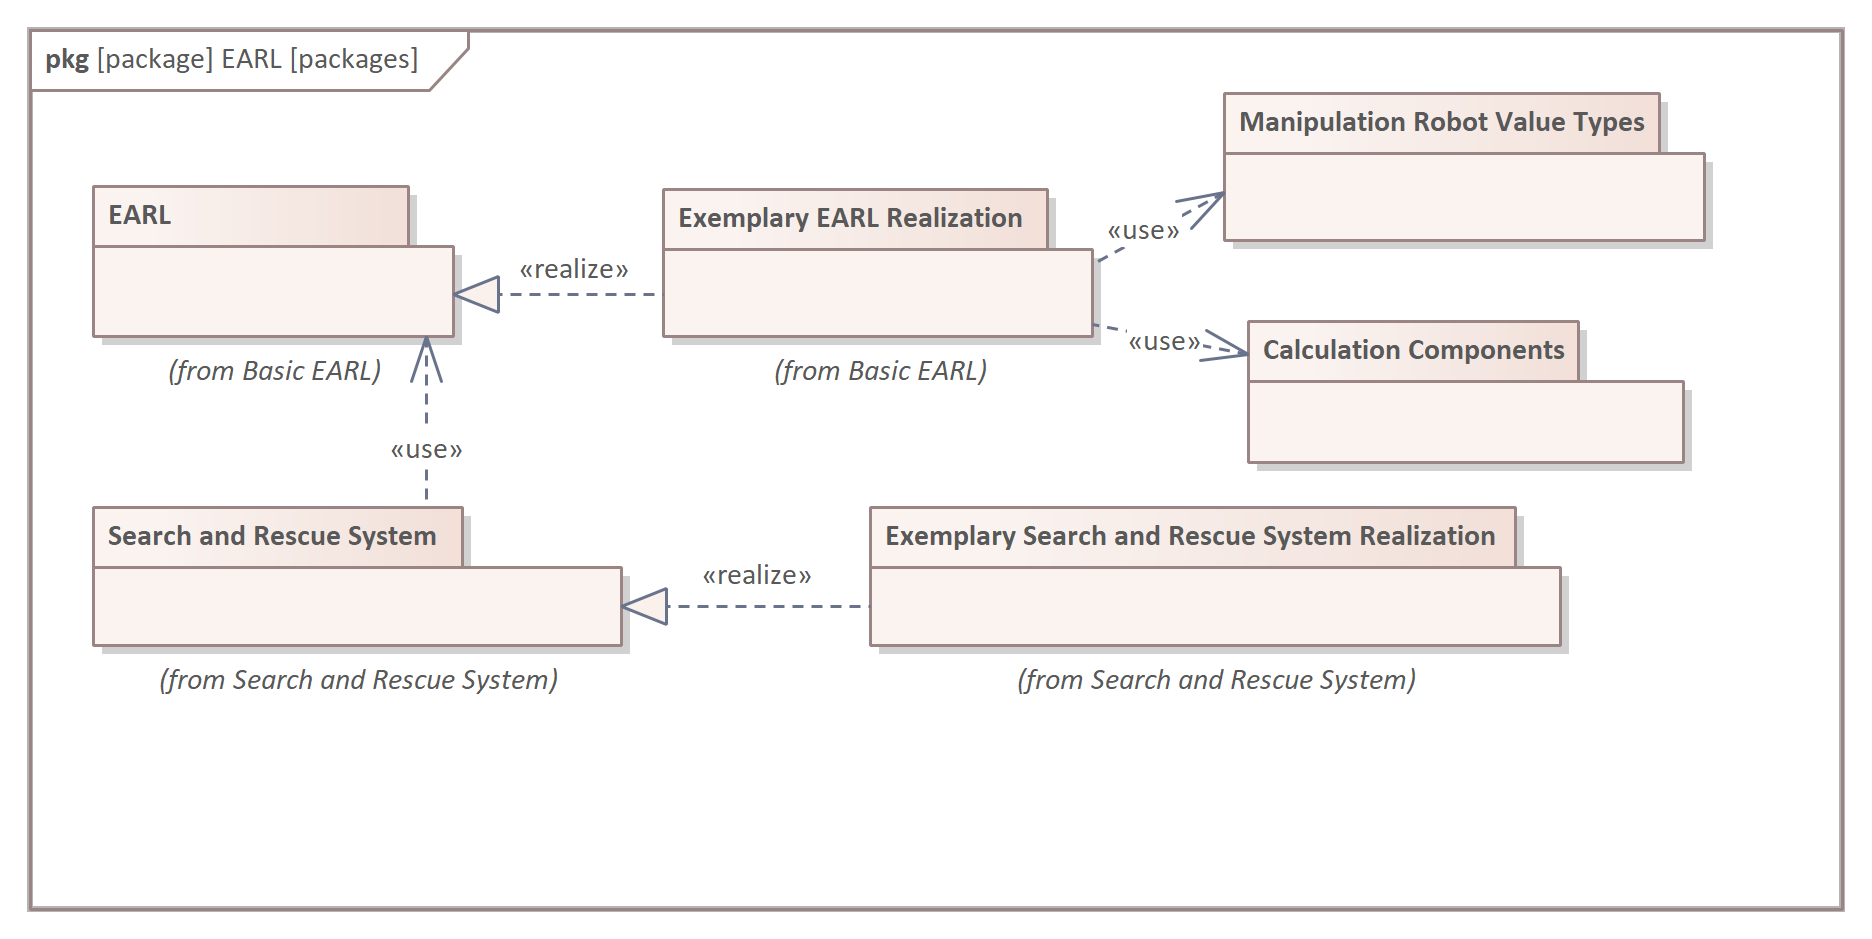
\includegraphics[width=0.9\columnwidth]{img/packages.png}}
		\end{center}
		\caption{\EARL{} packages dependencies}
		\label{fig:earl}
	\end{figure}
	
	
	 Although the large class of systems can be specified purely with the usage of the basic model presented further, the model can also be customised (e.g., \cite{winiarski-intent-20,karwowski2021hubero}) or incorporated into broader systems.
	 Some suggestions and examples are presented in Section~\ref{sec:customisations}. As the \EARL{} is constantly developed by its community, the list of major changes in \EARL{} current version is listed in Section~\ref{sec:major-changes}.

	\section{Model Formulation}
	\label{sec:ea-sysml}
	
	The model of a~system specified in \EARL{} is composed of concepts describing its structure and behaviour.
	The structure of the model is specified with \SysML{} \BlockDefinition{} \Diagrams{} (bdd) and \InternalBlock{} \Diagrams{} (ibd)~\cite{omg-sysml16}.
	For compactness and clarity of presentation the stereotypes are introduced that are provided as dedicated UML profile.
	The model is composed of a~set of diagrams. Each of the diagrams presents only a~part of the structure, however the whole set has to be consistent.The stereotypes names are long, hence descriptive, while parts' names are concise to reduce the space to point out the part and its context when it is convenient. 
	Some of the model constraints are defined by mathematical equations. 
		
	
	\subsection{System and Its Parts}
	\label{subsec:sys-a-subsys}
	
	\System{} is the most general \EARL{} concept. Its composition is defined in \Figure{}~\ref{fig:warstwa_systemu}. It	can contain a~number of \GroupsofAgents{}~$\ega{}$. A~\GroupofAgents{} is composed of at least one \Agent{}~$\ea{}$ and can constitute, e.g., a~Robot or a~part of the system executed on a~particular computer. The \GroupofAgents{} can also refer to other \GroupofAgents{} as $\ega{}$.
	%	 A~\BasicSystem{} may contain \Agents{} that are not elements of \GroupsofAgents{}, e.g.,\ an \Agent{} coordinating the work of a~group of Robots~\cite{zielinski-kka:2017}.
	\Agents{} are connected with $\eaa{}$ inter-agent communication \Links{}. Each $\eaa{}$ \Link{} can be referred by a~\GroupofAgents{}. In general, the \Links{} parts names are created by combining the source block part name at the beginning of the \Link{} part name and destination block part name at the end of the \Link{} part name.
	

	\begin{figure}[H]
		\centering
		\begin{center}
			{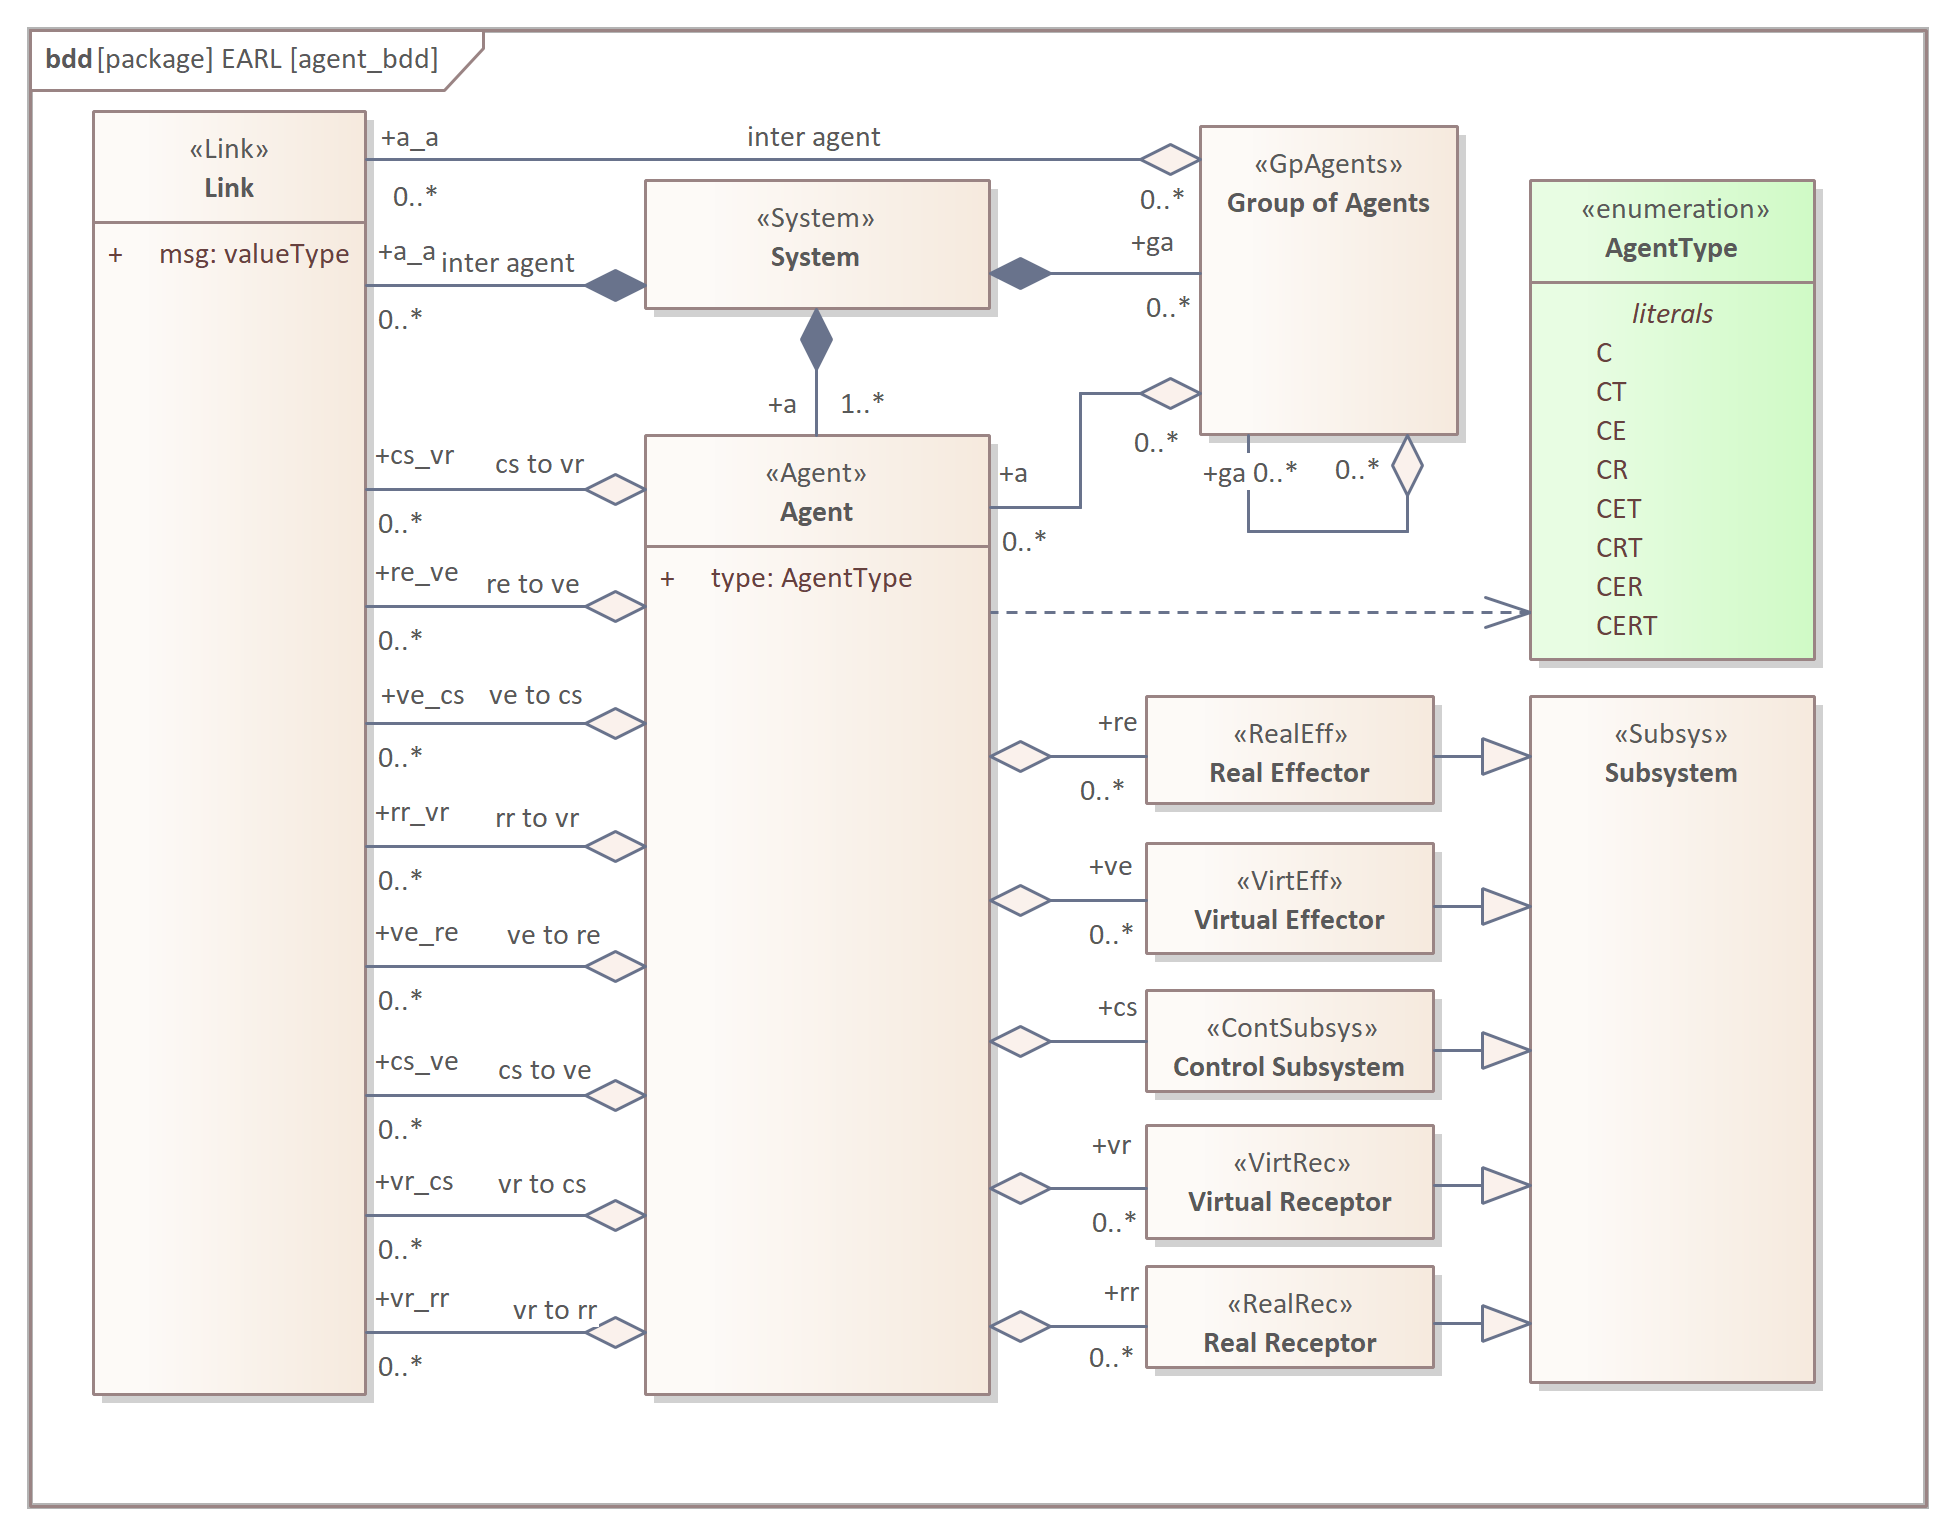
\includegraphics[width=.9\columnwidth]{img/basic_earl_model/agent_bdd.png}}
		\end{center}
		\caption{\System{} layer} 
		\label{fig:warstwa_systemu}
	\end{figure}
	
	In \cyberphysical{} systems an \Agent{} usually has a~physical body, thus it is an \EmbodiedAgent{}. 
	The composition of an \Agent{} is defined in \Figure{}~\ref{fig:warstwa_systemu}.
	The specific features of robotics, where an \Agent{} can take on various roles, from real-time control, through sensor data processing, to execution of computationally demanding
	tasks~\cite{stigmergic:2009}, require its decomposition into various types of \Subsystems{} and specialised \Links{} between them.
	The variety of link names was introduced to distinguish the types of \Subsystems{} that communicate with each other and the direction of data transmission.
	The blocks cardinality presented in~\Figure{}~\ref{fig:warstwa_systemu} is general,
	but particular system composition may introduce more strict constraints according to the extra rules presented further.
	
	There are five different specialisations of \Subsystems{} (right side of \Figure{}~\ref{fig:warstwa_systemu}). The main one (indispensable for an \Agent{}) is a~\ControlSubsystem{}~$\ecs{}$, which coordinates the \Agentapostrofs{} \Subsystems{} and communicates with other \Agents{}.
	\RealEffectors{}~$\ere{}$ are \Subsystems{} which affect the environment, whereas \RealReceptors{}~$\err{}$ (exteroceptors) gather information from the environment. \VirtualSubsystems{} (\VirtualReceptors{}~$\evr{}$ and \VirtualEffectors{}~$\eve{}$) supervise the work of \RealSubsystems{}. Therefore, the \RealSubsystems{} of a~particular type, cannot exist without Virtual ones and vice versa, see Equation~\eqref{eq:ss-quantity-constraint}. 
	\begin{equation}
	|\evr{}| \geqslant 1 \iff |\err{}| \geqslant 1,\;\;\;
	|\eve{}| \geqslant 1 \iff |\ere{}| \geqslant 1.
	\label{eq:ss-quantity-constraint}
	\end{equation}
	Inequalities Equation~\eqref{eq:ss-quantity-constraint} represents the necessary conditions ensuring the preservation of system integrity.
	Additional constraints have to be imposed on the number of \Subsystems{} due to the specificity of inter-subsystem communication \Links{} (Section~\ref{sec:communication}).
	
	The \Links{} and \Subsystems{} are composed in System (\Figure{}~\ref{fig:system_layer_compos_bdd}) and aggregated in \Agent{} to make it possible to logically share them between \Agents{}.
	
	\begin{figure}[H]
		\centering
		\begin{center}
			{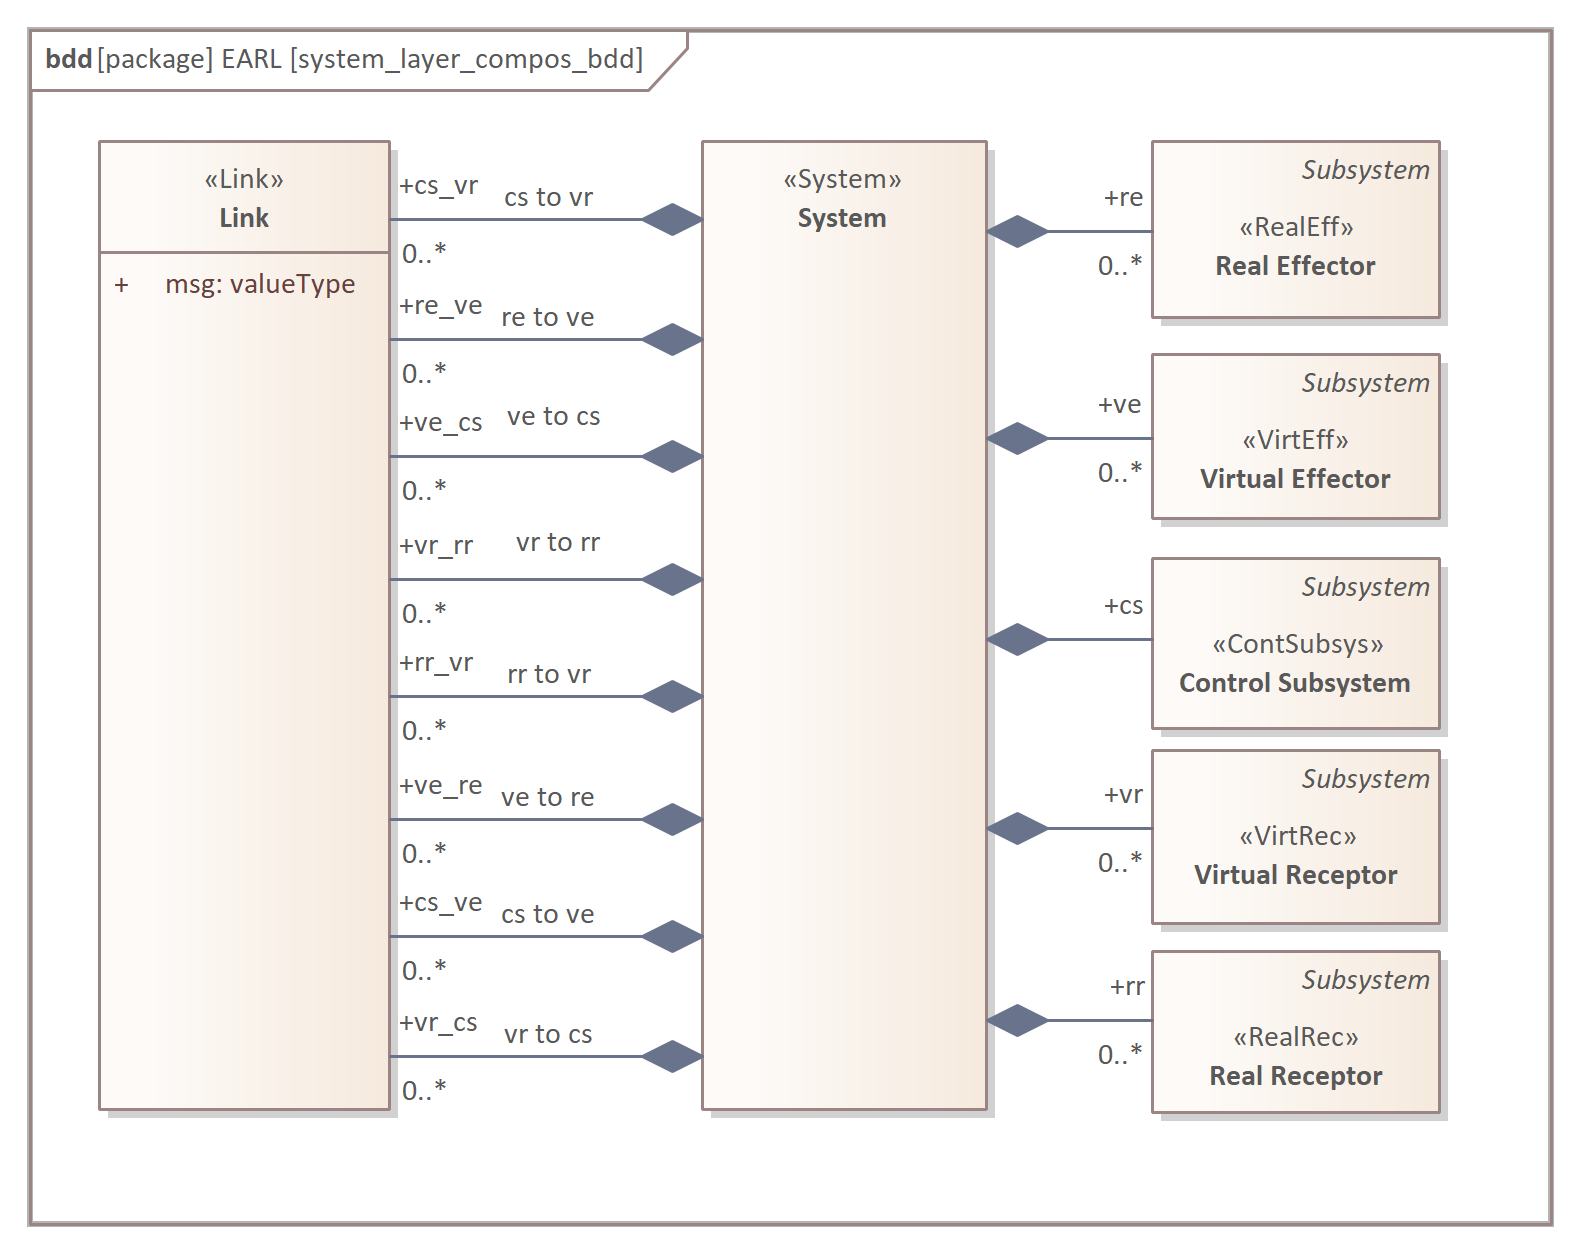
\includegraphics[width=.8\columnwidth]{img/basic_earl_model/system_layer_compos_bdd.png}}
		\end{center}
		\caption{\System{} and composed \Links{} and \Subsystems{}} 
		\label{fig:system_layer_compos_bdd}
	\end{figure}
		
	The \GroupofSubsystems{} (\Figure{}~\ref{fig:grupa_podsystemowa}) was introduced for the purpose of alternative presentation (view) of \System{} or \Agent{} structure by grouping the \Subsystems{} and \Links{} between them. 
		
		
\begin{figure}[H]
	\centering
	\begin{center}
		{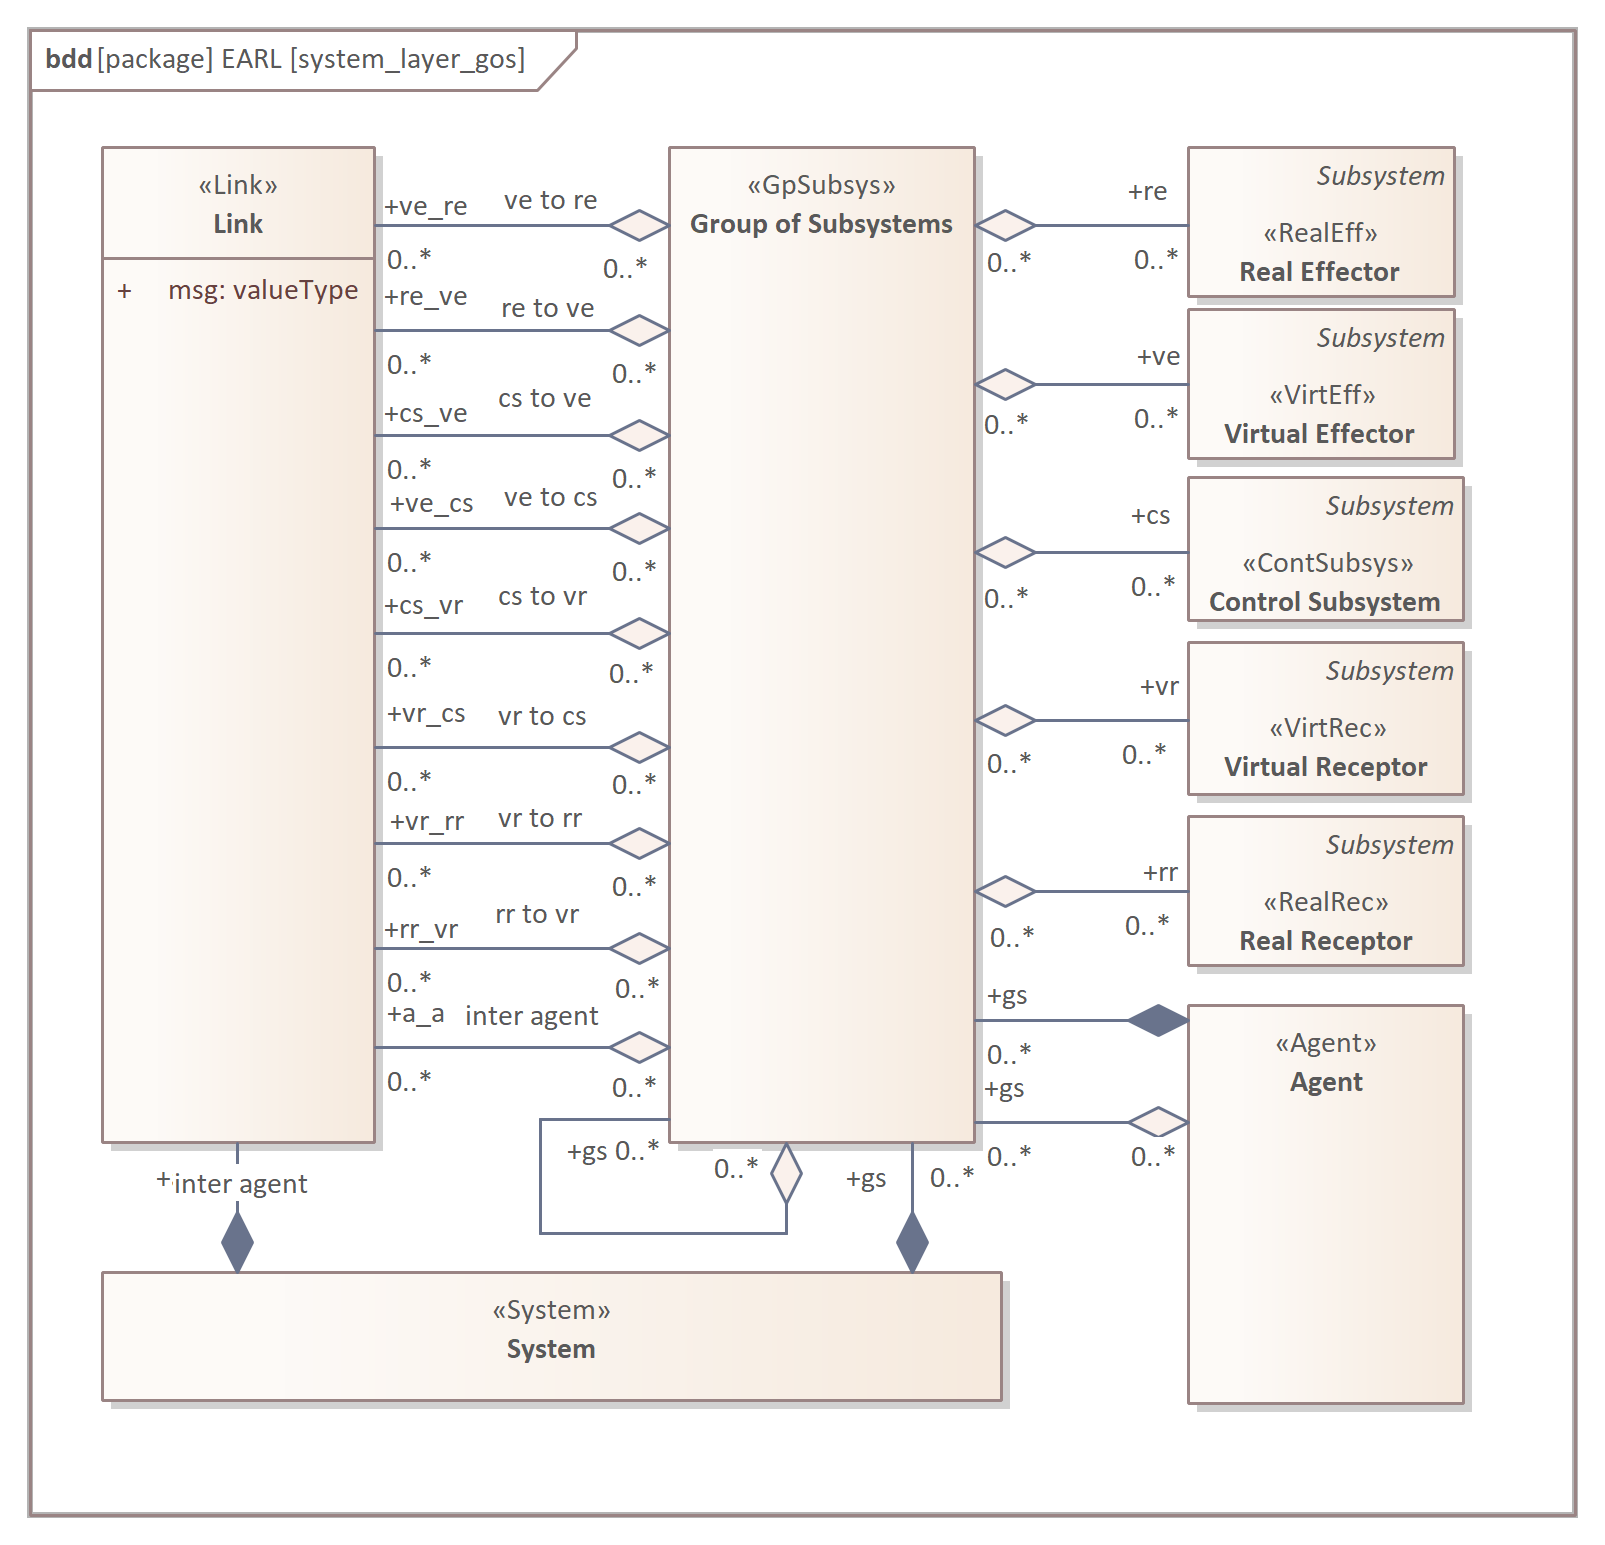
\includegraphics[width=.8\columnwidth]{img/basic_earl_model/system_layer_gos.png}}
	\end{center}
	\caption{\GroupofSubsystems{}} 
	\label{fig:grupa_podsystemowa}
\end{figure}
		
If the \Subsystems{} from various \Agents{} are grouped into the single \GroupofSubsystems{}, then this group is a~part of \System{} labelled as $\egs{}$ that can be also aggregated as a~reference $\egs{}$ into \Agents{}. 
%	In that case the \GroupofSubsystems{} can be of \textbf{MAF} type (Multi Agent Full), when it aggregates all of the \Subsystems{} of aggregated \Agents{}, or of \textbf{MA} type (Multi Agent) when not all the \Subsystems{} of the aggregated \Agents{} are aggregated.
 The \Subsystems{} of single \Agent{} can aggregate into its internal part -- \GroupofSubsystems{} $\egs{}$.
%  of \textbf{IA} type (Intra Agent)
The \GroupofSubsystems{} can also refer to other \GroupofSubsystems{} as $\egs{}$. As the example the \GroupofSubsystems{} can aggregate the \Subsystems{} that run in a~single operating system's process, use the same communication medium (e.g., WiFi), or form a~particular robot control system.
	
The \GroupofLinks{} (\Figure{}~\ref{fig:group_of_links_bdd}) was introduced for the purpose of aggregated presentation of communication links between various blocks. It aggregates \Links{}. Especially, in opposition to particular \Links{}, the \GroupofLinks{} can represent both uni and bi directional communication. The \GroupofLinks{} can be composed or aggregated into various blocks as $\egl{}$. The recursive self reference of \GroupsofLinks{} is also possible.
	
\begin{figure}[H]
	\centering
	\begin{center}
		{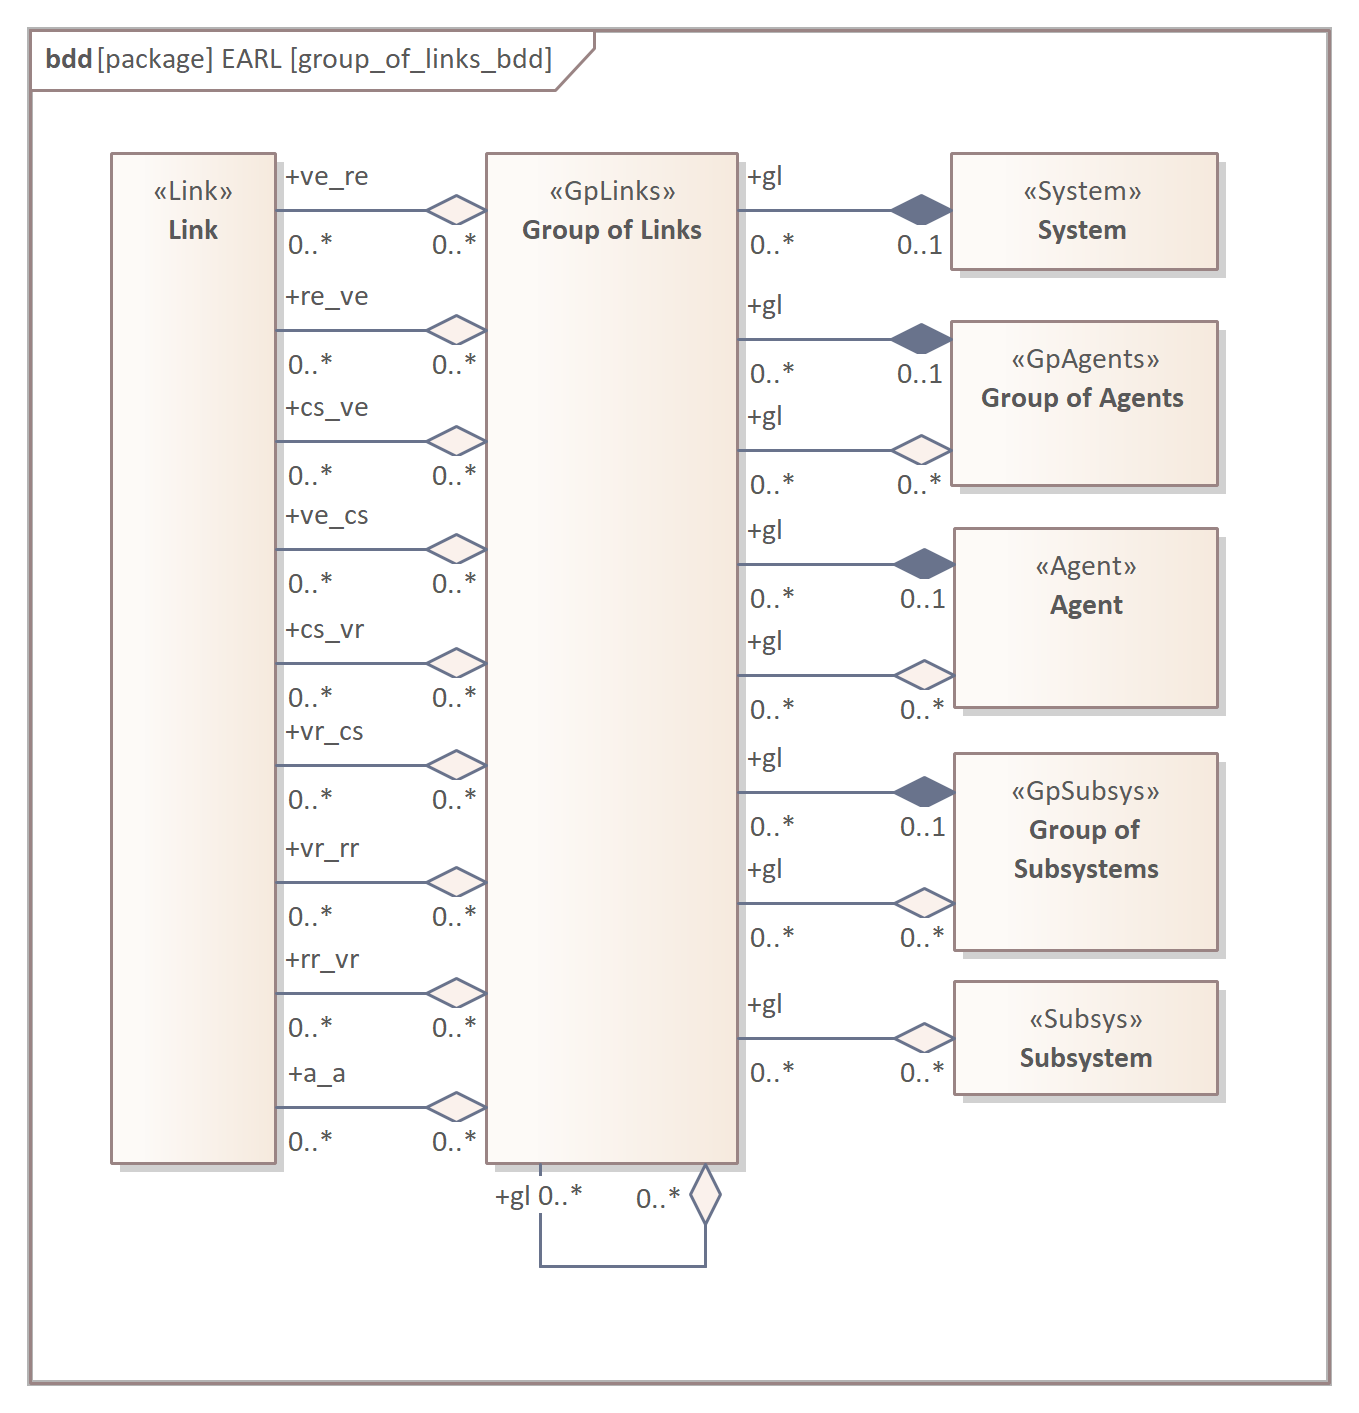
\includegraphics[width=.65\columnwidth]{img/basic_earl_model/group_of_links_bdd.png}}
	\end{center}
	\caption{\GroupofLinks{}} 
	\label{fig:group_of_links_bdd}
\end{figure}	

	
	\subsection{\Subsystem{} and its Parts}
	The composition of a~Subsystem{} is defined in~\Figures{}~\ref{fig:warstwa_podsystemu},~\ref{fig:podsystem_hfsm}~and~\ref{fig:subsystem_buffers}. It contains \InputBuffers{}~$\eib{}$ and \OutputBuffers{}~$\eob{}$,
	\InternalMemory{}~$\emb{}$ and other entities that are used to model both structural and behavioural aspects of a~Subsystem{},
	i.e., \Fsm{}~$\efsm{}$ (\FiniteStateMachine{}), multiple internal \FiniteStateMachines{}~$\eifsm{}$, \Predicates{}~$\ep{}$, \BasicBehaviours{}~$\ebb{}$ and \PrimitiveTransitionFunctions{}~$\epf{}$.
	
	\begin{figure}[H]
		\centering
		\centering
		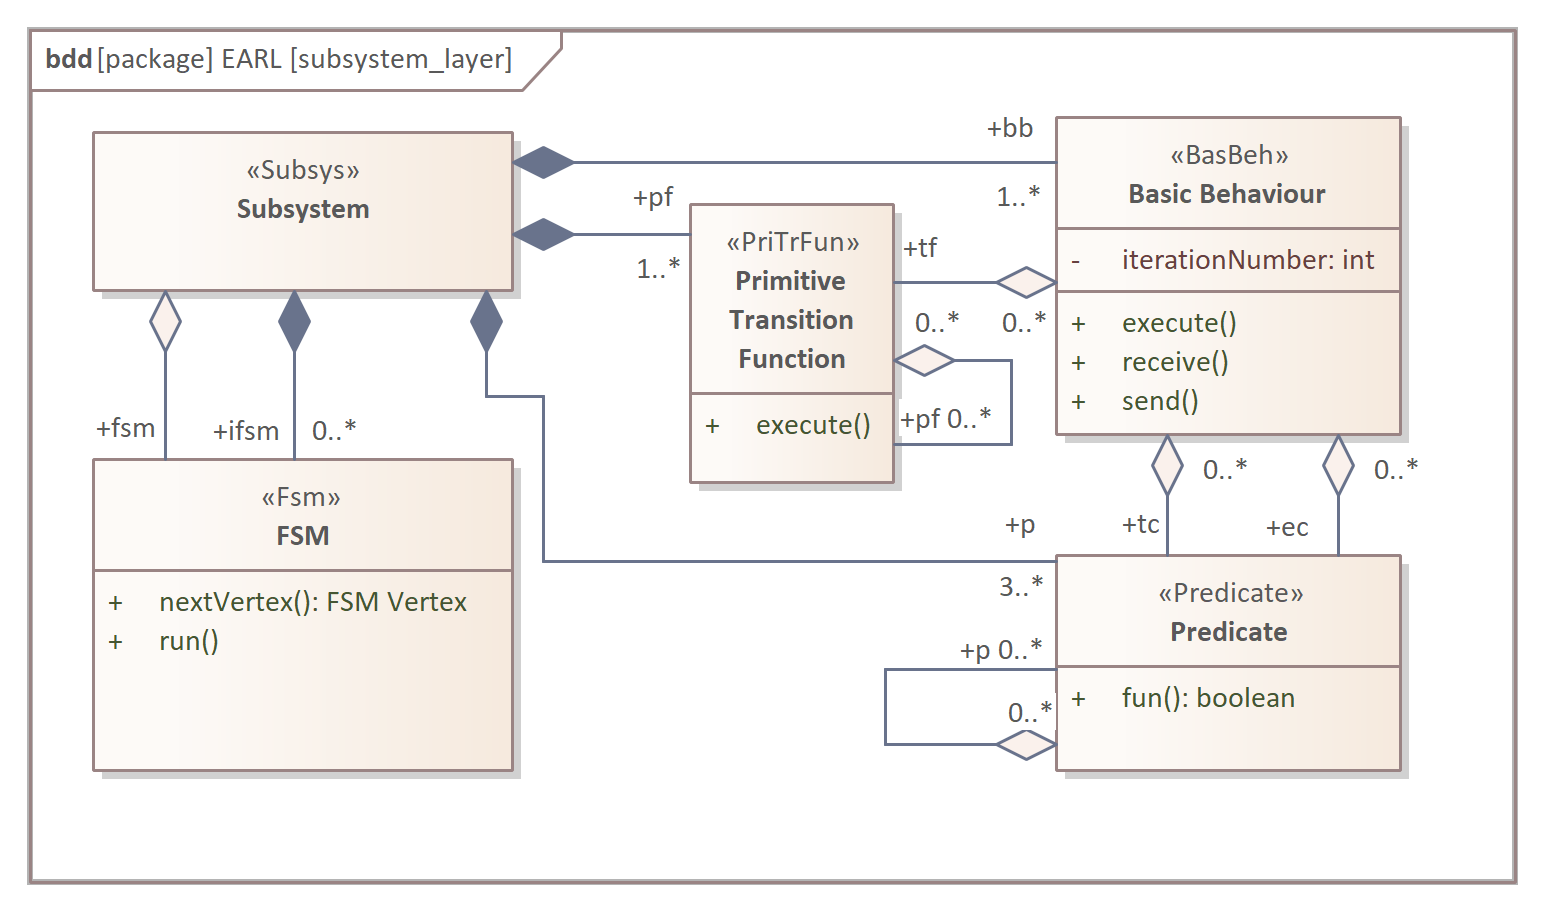
\includegraphics[width=.8\textwidth]{img/basic_earl_model/subsystem_layer.png}
		\caption{\Subsystem{} and its parts (Input, Output \Buffers{}, \InternalMemory{} and Hierarchical FSM are excluded)}
		\label{fig:warstwa_podsystemu}
	\end{figure}	

	\begin{figure}[H]
		\centering
		\centering
		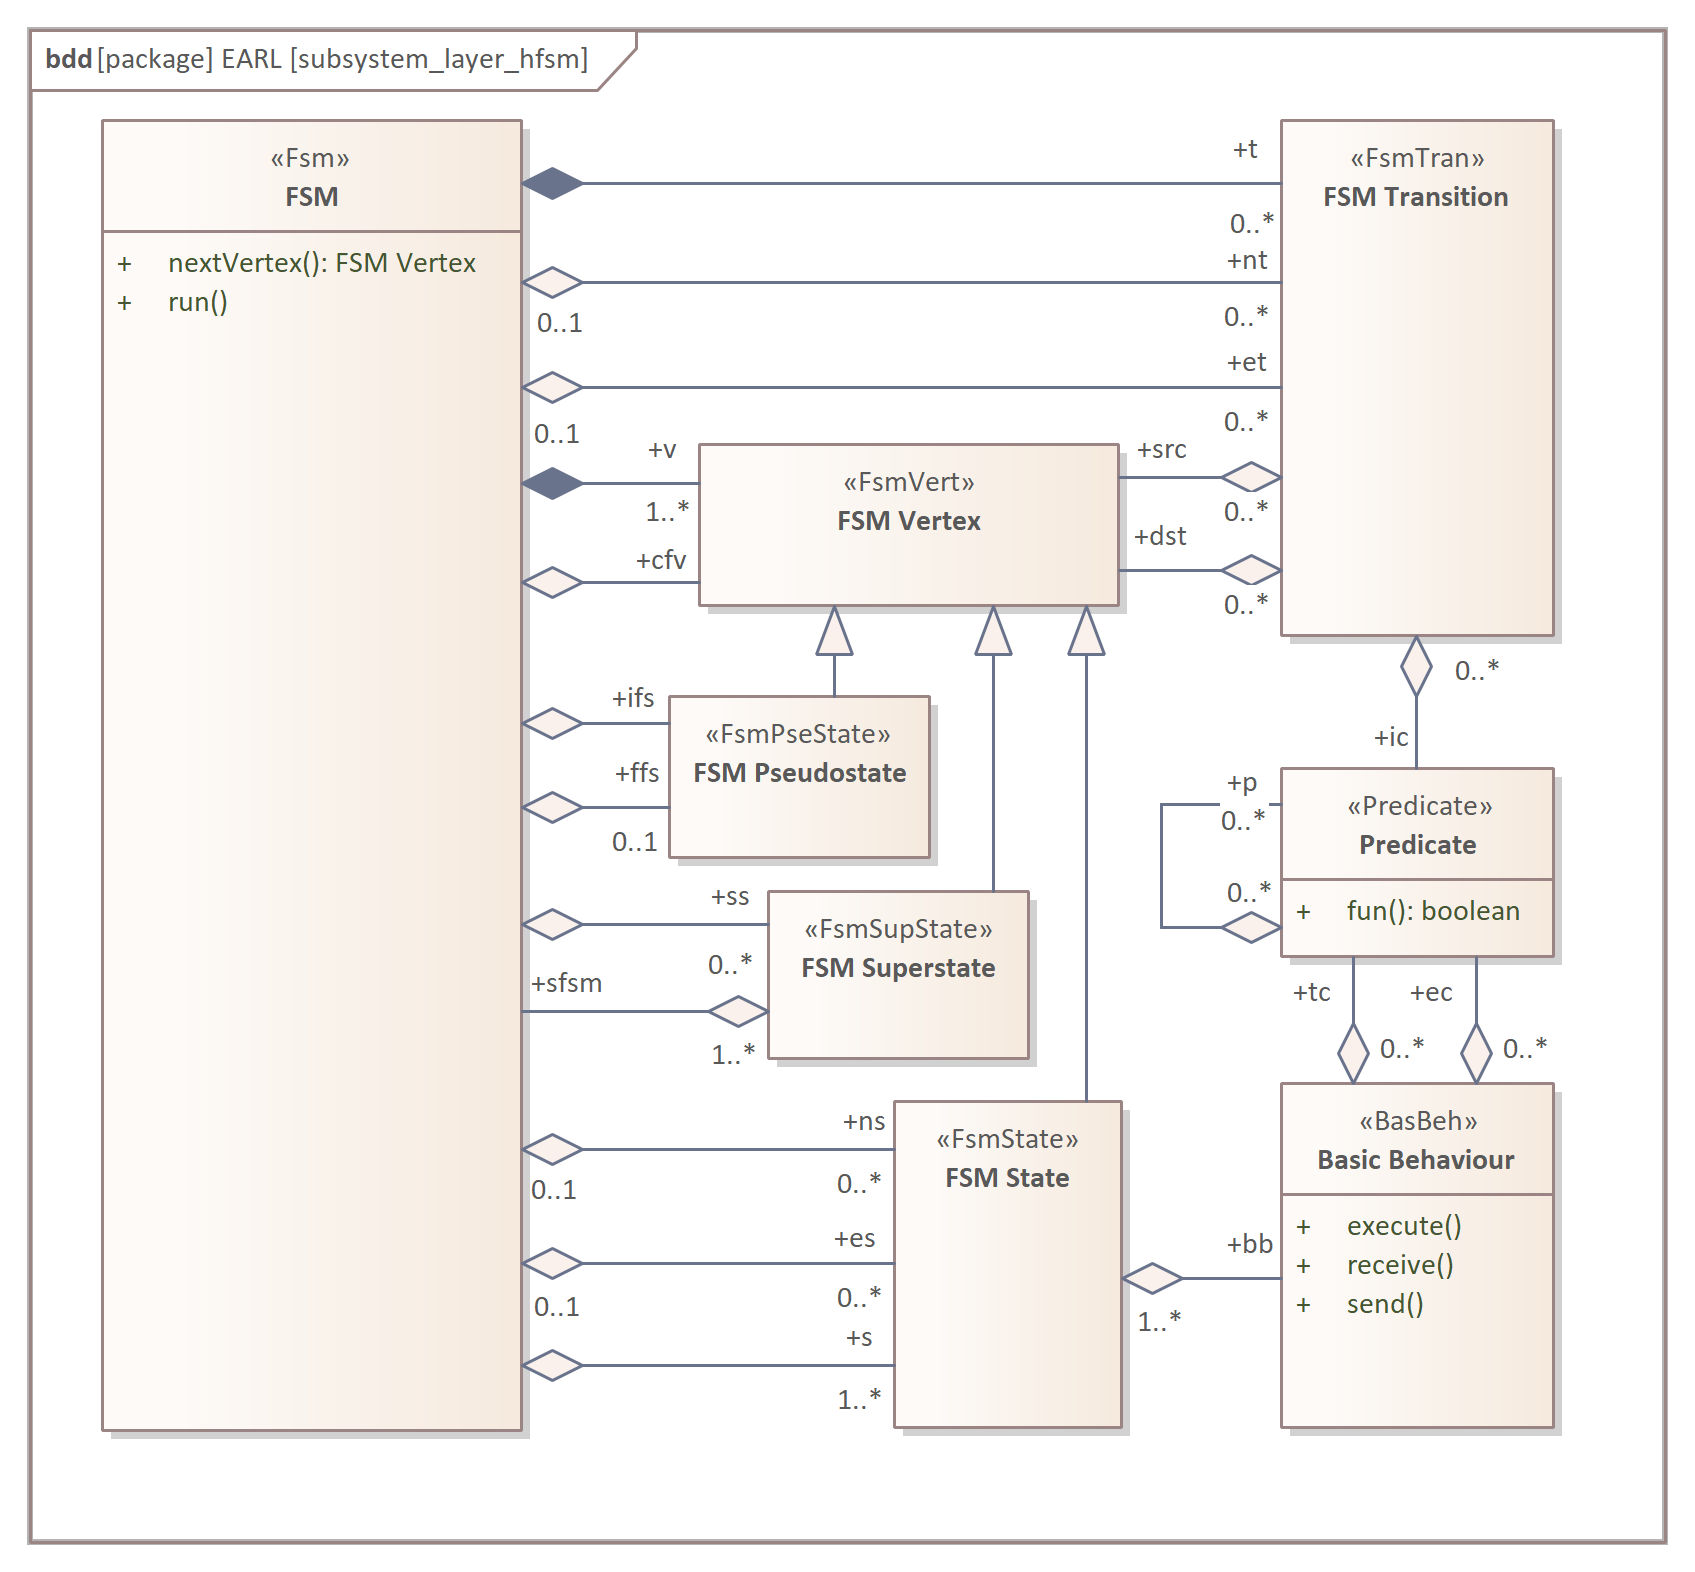
\includegraphics[width=.75\textwidth]{img/basic_earl_model/subsystem_layer_hfsm.png}
		\caption{\Subsystem{} hierarchical FSM}
		\label{fig:podsystem_hfsm}
	\end{figure}	
	
	\Figure{}~\ref{fig:re_buffers} depicts relations between a~particular \Subsystem{} and its communication \Buffers{}.
	The communication constraints depicted in Section~\ref{sec:communication} cause that each \VirtualReceptor{} or \VirtualEffector{}
	must have at least one \InputBuffer{} and one \OutputBuffer{}. A~\RealEffector{} needs at least one \InputBuffer{} to receive commands,
	and a~\RealReceptor{} needs at least one \OutputBuffer{} to send sensory data.
	
	\begin{figure}[H]
		\centering
		\def\myheight{7.5cm}
		\subfloat[\label{fig:subsystem_buffers}]{ 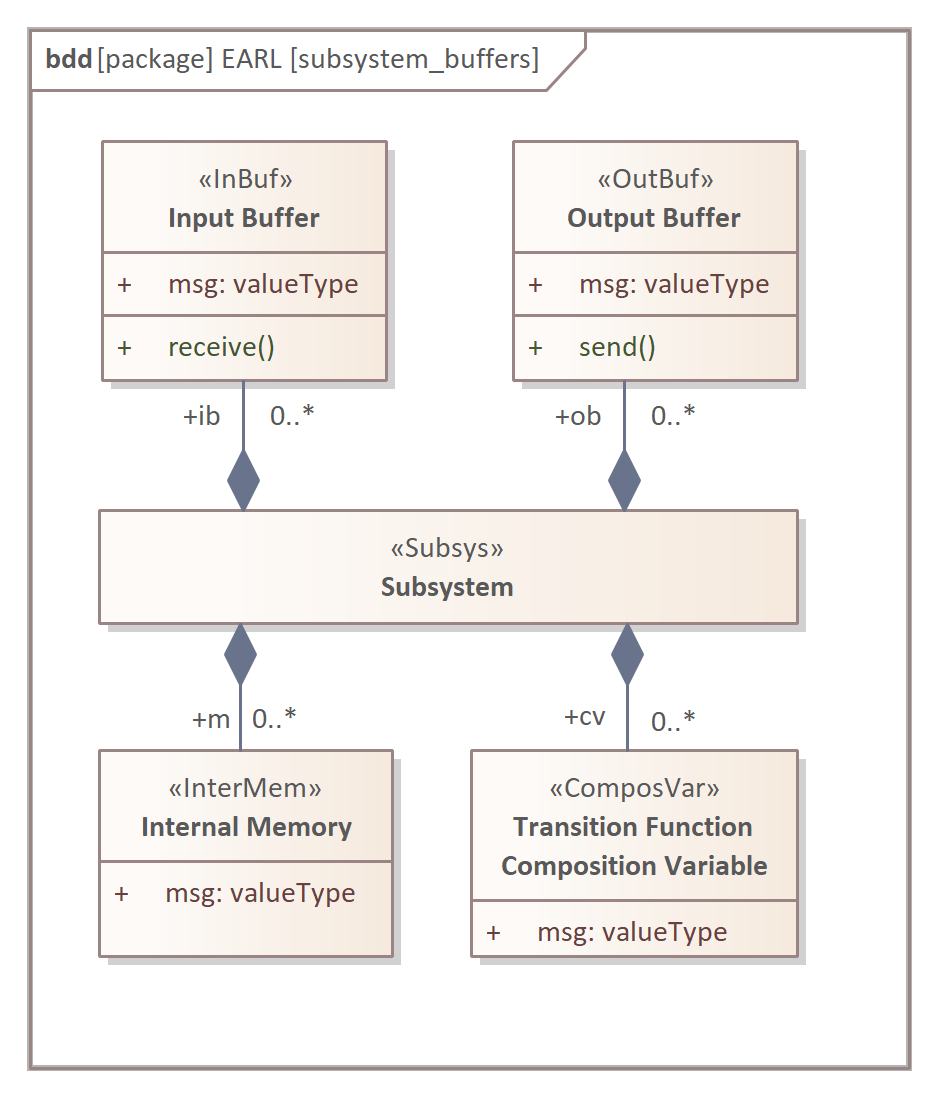
\includegraphics[height=\myheight]{img/basic_earl_model/subsystem_buffers.png}} \quad
		\subfloat[
		\label{fig:re_buffers}]{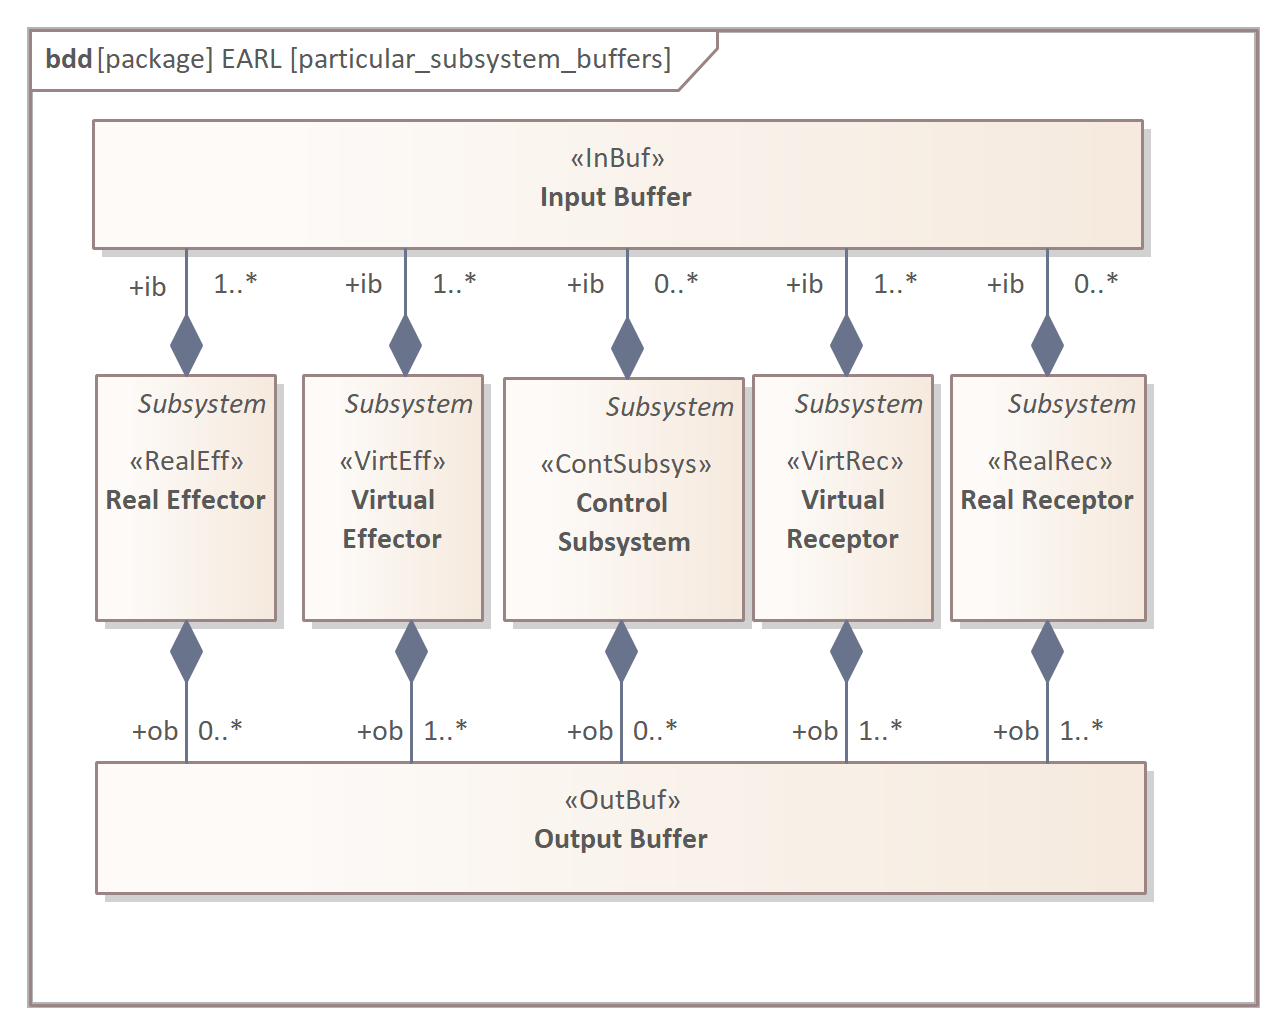
\includegraphics[height=\myheight]{img/basic_earl_model/particular_subsystem_buffers.png}}
		\caption{\Subsystems{} and \Buffers{}. (\textbf{a}) \Subsystem{} Buffers and Internal Memory; (\textbf{b}) Relation of particular \Subsystems{} to communication \Buffers{}}
		\label{fig:ss-buf}
	\end{figure}
	
	\Ib{}, \Ob{} and \Mb{} are defined analogically as in~\cite{Trojanek:phd2012}.
	Each \Buffer{} contains a~data structure $msg$, which stores data of type \ValueType{}.
	The \ValueType{} can be defined either as a~primitive type or a~composite and nested structure.
	\InputBuffer{} possesses an operation $\receive{}$, which enables communication with \OutputBuffers{}, and stores the received data in the \InputBuffer{}.
	Analogically, \OutputBuffer{} has a~$\send{}$ operation, which dispatches the data stored in the \OutputBuffer{} to the connected \InputBuffers{}.
	\InternalMemory{} stores $\emsg{}$,	which is a~value of type \ValueType{}. \TransitionFunctionCompositionVariables{} were introduced for the purpose of Communication between \PrimitiveTransitionFunctions{} to compose \TransitionFunction{}. \TransitionFunctionCompositionVariable{}, analogically to \InternalMemory{}, stores $\emsg{}$, which is a~value of type \ValueType{}. 
	Various forms of communication between \Subsystems{} have been described in the paper~\cite{hexel-jint2019}.
	
	Similarly to~\cite{robotml,Kornuta:13_irs}, the \EARL{} \Subsystem{} structural model contains a~\FiniteStateMachine{} (\Fsm{}) that determines its
	activities (\Figure{}~\ref{fig:warstwa_podsystemu}). The \Fsm{} is a~graph defined by a~set $\ev{}$ of \FsmVertices{} and a~set $\et{}$ of \FsmTransitions{}. Current \FsmVertex{} is called $\ecfv{}$. There are three types of \FsmVertices{}. The first one is \FsmPseudostate. Each \Fsm{} can have one initial \FsmState~--~$\eifs{}$ and zero or one final \FsmState{}~--~$\effs{}$. Those states point the initial and final \FsmVertex{}. The second type is \FsmSuperstate{}~--~$\ess{}$. Each \Fsm{} can aggregate many $\ess{}$. Each \FsmSuperstate{} aggregates one \Fsm{} called $\esfsm{}$. The last one is \FsmState{}. Each \FsmState{} aggregates one \BasicBehaviour{}. The \FsmStates{} can be aggregated into two groups: normal \FsmStates{} $\ens{}$ and error handling \FsmStates{} $\ees{}$. Similarly \FsmTransitions{} can be aggregated into: normal \FsmTransitions{} $\ent{}$ leading to normal \FsmStates{} and error handling \FsmTransitions{} $\eet{}$ leading to error handling \FsmStates{}. A~\Predicate{} specified in operation $fun()$ of \FsmTransitions{} $\ent{}$ should satisfy at least the \Predicate{} \eqref{eq:p-ec}
		\begin{equation}
		\ep{errTran}.fun() := \emi{errorTransiton}.\emsg{},
		\label{eq:p-ec}
	\end{equation}	
	 and analogically a~\Predicate{} of \FsmTransitions{} $\eet{}$ should satisfy at least the \Predicate{} \eqref{eq:p-n-ec}
	
	\begin{equation}
		\neg \ep{errTran}.fun() := \neg \emi{errorTransiton}.\emsg{}.
		\label{eq:p-n-ec}
	\end{equation}			
	
	\Figure{}~\ref{fig:run} defines how the $\run{}$ operation of \Fsm{} works. In each moment of the \Subsystem{} running there is exactly one \FsmVertex{} active. It is called current \FsmVertex{} -- $\ecfv{}$. The \Fsm{} starts in the initial \FsmState{} $\eifs{}$. In each iteration of $\run{}$ operation the type of $\ecfv{}$ is checked. If $\ecfv{}$ is of:
	\begin{itemize}
		\item \FsmState{} type, it means that $\ecfv{}$ is associated with the \BasicBehaviour{} $\ebb{}$. Consequently the $\ecfv{}.\ebb{}.\execute{}$ operation executes a~behaviour associated with the current vertex. Next, the function $\nextvertex{}$ choose new current \FsmVertex{} -- $\ecfv{}$.
		\item \FsmPseudostate{} type, there is a~question if it is initial state or final state. It it is initial state, the function $\nextvertex{}$ choose new current \FsmVertex{} -- $\ecfv{}$. Otherwise, the action of $\run{}$ operation is finished.
		\item \FsmSuperstate{} type, the $\run{}$ operation of sub-automata -- $\ecfv{}.\esfsm{}.\run{}$ -- is executed.
	\end{itemize}
	
	
	\FsmTransition{} (\Figure{}~\ref{fig:warstwa_podsystemu}) is defined by the source and destination \FsmStates{}
	as well as the associated \InitialCondition{}, i.e., \Predicate{} $\eic{}$.
	
	\begin{figure}[H]
		\centering
		\begin{center}
			{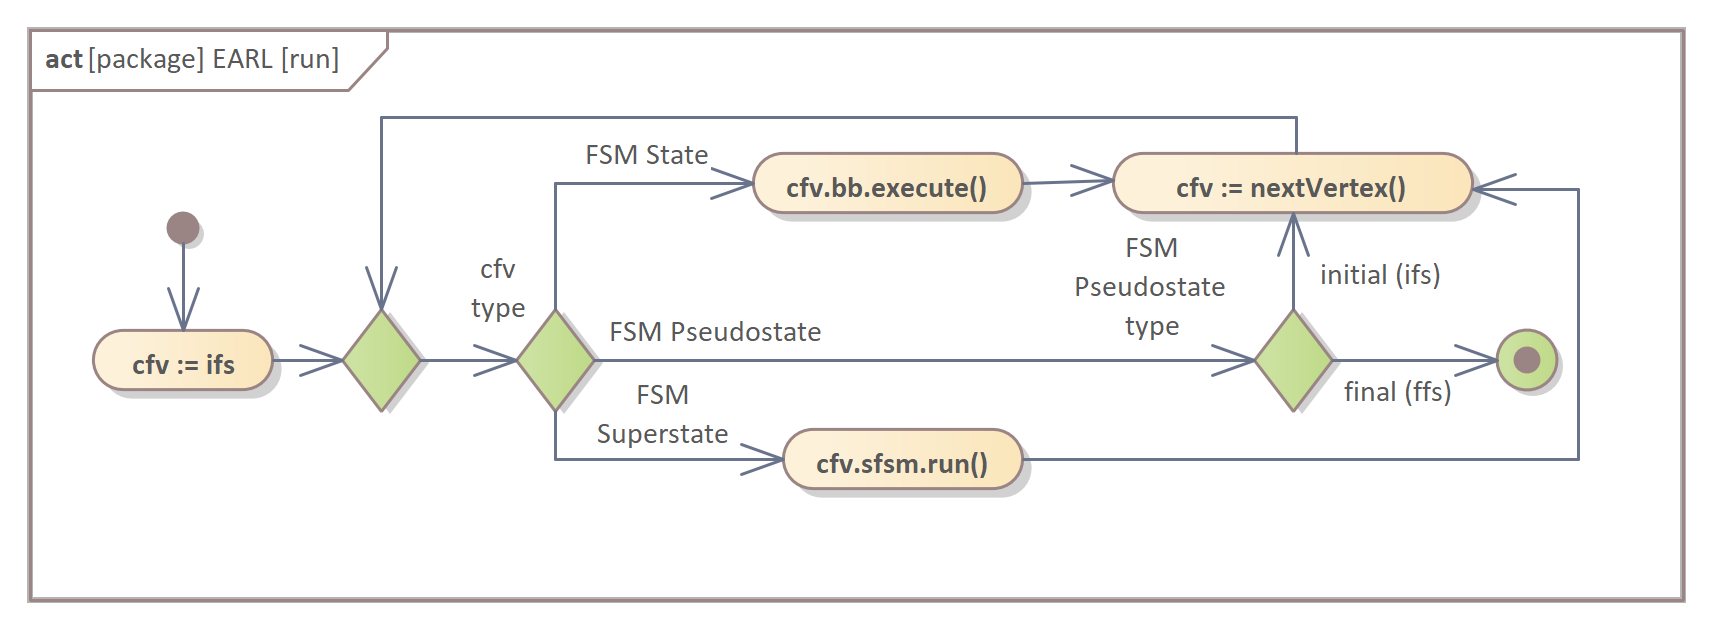
\includegraphics[width=0.85\columnwidth]{img/basic_earl_model/run.png}}
		\end{center}
		\caption{\Fsm{}.$\run{}$ operation}
		\label{fig:run}
	\end{figure}	
	
	
	In the following part of the documentation a~\SysML{} dot ``.'' notation~\cite{omg-sysml16} is used to depict the nesting of the part instances as well as other block properties.
	The dot ``.'' can be treated as an extraction operator. It is assumed that if a~specific instance of a~part is not indicated, the set of all instances of the part is
	taken into account.
	In particular, if there is only one instance, there is no need to name it explicitly, only the part name is needed. The same rule applies to references.
	As the particular parts compose objects of the same type, they can be interpreted as sets in mathematical formulas. 
	The composition of a~\BasicBehaviour{} is defined in \Figure{}~\ref{fig:warstwa_podsystemu}.
	The~\BasicBehaviour{} includes its transition function $\etf{}$ which is referred to one of the \PrimitiveTransitionFunctions{}; a~\TerminalCondition{} $\etc{}$ , which is a~\Predicate{} determining when the execution of the \BasicBehaviour{} should terminate; and an~error condition $\eec{}$, which is a~\Predicate{}
	indicating that an error has been detected in the execution of the \BasicBehaviour{}. \BasicBehaviour{} also posses an $\execute{}$ operation (\Figure{}~\ref{fig:eaa}).
	
	\begin{figure}[H]
		\centering
		\begin{center}
			{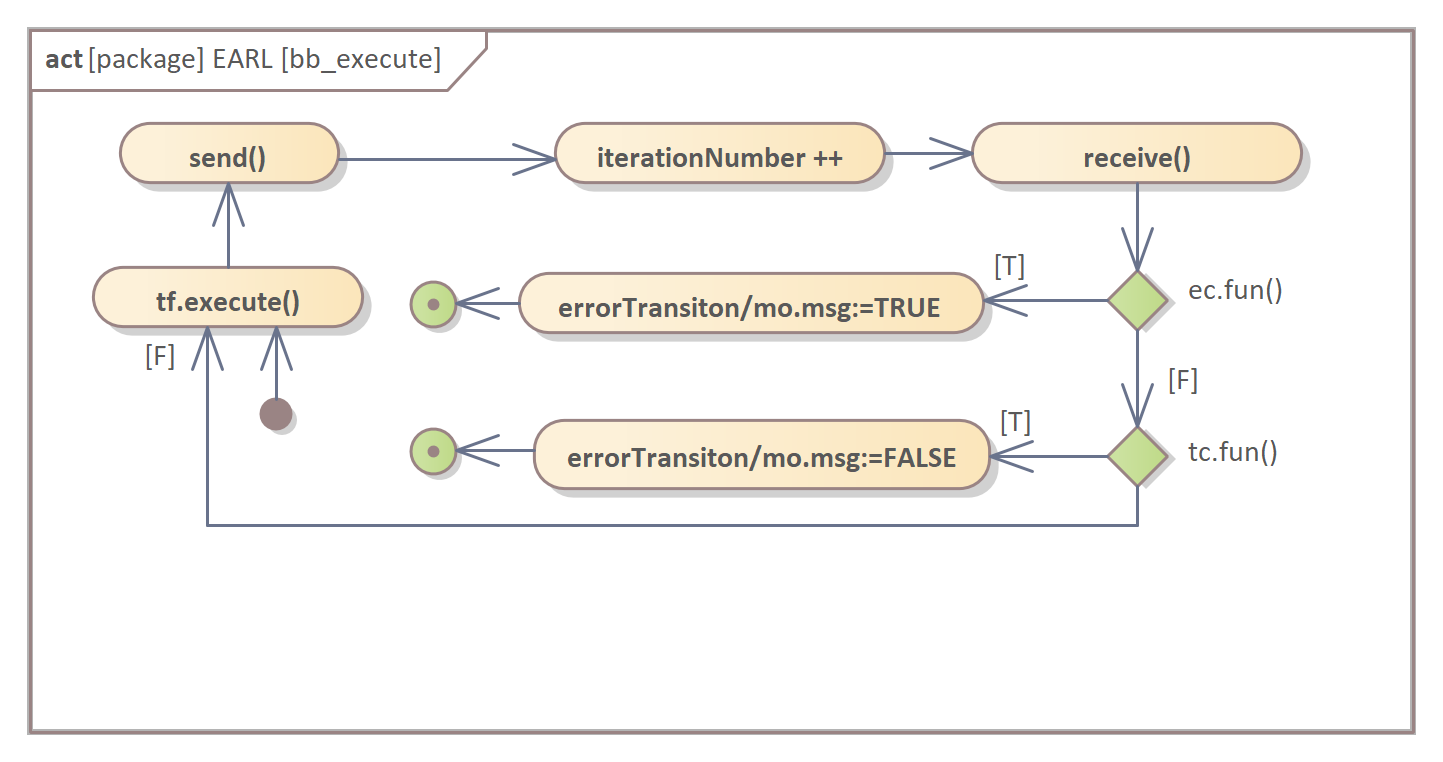
\includegraphics[width=0.7\columnwidth]{img/basic_earl_model/bb_execute.png}}
		\end{center}
		\caption{\BasicBehaviour{}.$\execute{}$ operation}
		\label{fig:eaa}
	\end{figure}	
	
	That operation, first executes a~transition function~$\etf{}.\execute{}$,
	then all calculated \OutputBuffers{} values are sent out by $\send{}$. Next, $\eiterationnumber{}$ is incremented, and
	$\receive{}$ gets new values into \InputBuffers{}. Finally, \ErrorCondition{}~$\eec{}.\fun{}()$ and
	\TerminalCondition{}~$\etc{}.\fun{}()$ are tested. If both values are false, a~new iteration inside \BasicBehaviour{} $execute()$ operation is performed.
	Otherwise, $\emo{errorTransiton}.\emsg{}$ is set, \BasicBehaviour{} $execute()$ $operation$ ends and the \Fsm{} $\run{}$ operation designates the next \FsmState{} (\Figure{}~\ref{fig:run}).

	
	The composition of a~\PrimitiveTransitionFunction{} is defined in \Figure{}~\ref{fig:warstwa_podsystemu}.
		It refers to \InputBuffers{}, \OutputBuffers{} as well as \Subsystem{} \InternalMemory{}~(\Figure{}~\ref{fig:buffer_usage}).
		
	\begin{figure}[H]
		\centering
		\begin{center}
			{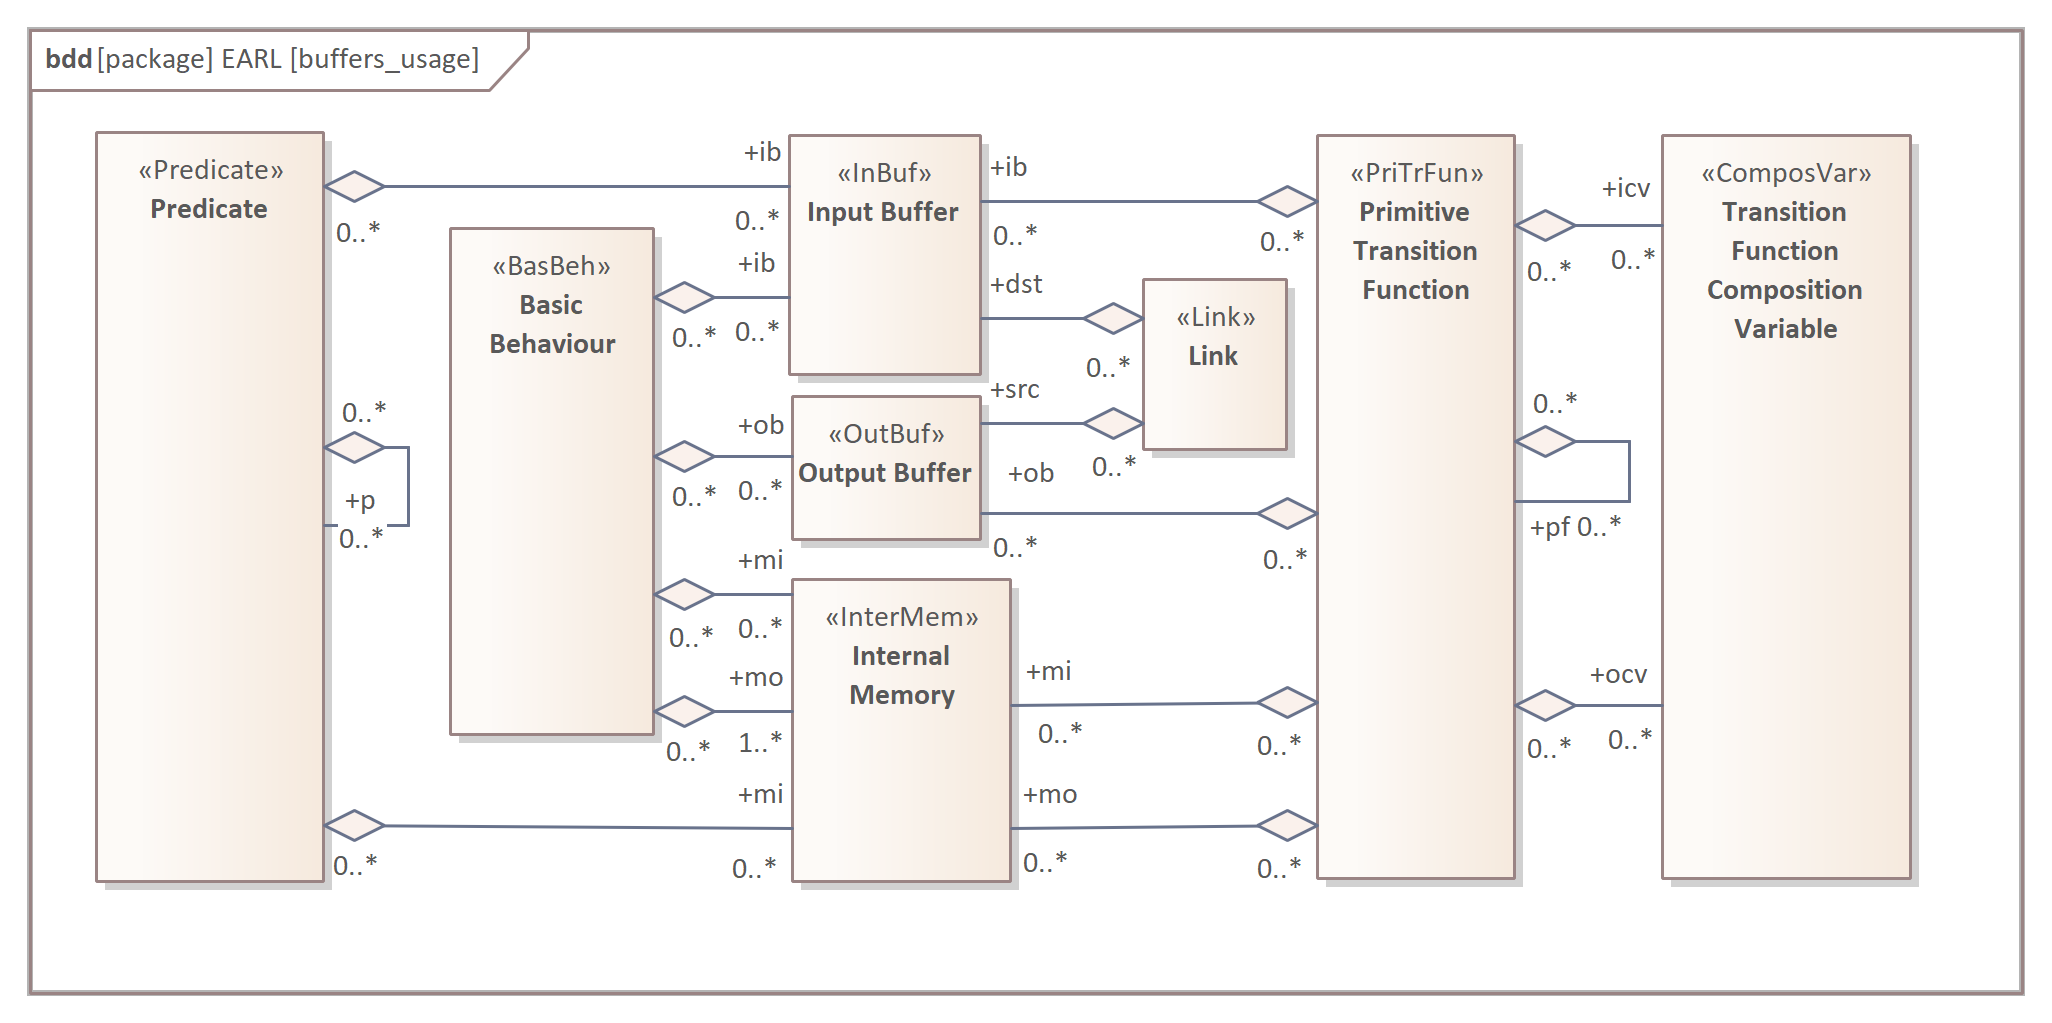
\includegraphics[width=\columnwidth]{img/basic_earl_model/buffers_usage.png}\label{aaa}}
		\end{center}
		\caption{The utilisation of \Buffers{}, \TransitionFunctionCompositionVariables{} and \InternalMemory{} by: \PrimitiveTransitionFunction{}, \Predicate{} and \Links{}}
		\label{fig:buffer_usage}
	\end{figure}	
		
		
	A~\PrimitiveTransitionFunction{} can read from the \InternalMemory{} (using the $\emi{}$ reference) or write to it (using the $\emo{}$ reference) and analogically read from the \TransitionFunctionCompositionVariable{} (using the $\eicv{}$ reference) or write to it (using the $\eocv{}$ reference).  It can aggregate other \PrimitiveTransitionFunctions{}. The aggregation can be modelled by directed graph, in case of \PrimitiveTransitionFunctions{} aggregation cycles are not allowed. Such an aggregation sometimes reduces the redundancy of the specification, making it more comprehensible. Moreover, if the implementation of the specified system is based on components, a~\PrimitiveTransitionFunction{} can be identified with a~separate component or a~set of components~\cite{dudek:2016-automation,mmar_winiarski_multibehavioral-2016}.
	The \PrimitiveTransitionFunction{} algorithm is executed by an $\epf{}.\execute{}$ operation. It can use a.o. components from the \CalculationComponentspkg{} Package (\Figure{}~\ref{fig:earl}).	The concept of the \EmbodiedAgent{} introduces no restrictions on how to implement this operation.
	
%	 The other two operations, i.e. $\epf{}.\send{}$ and $\epf{}.\receive{}$ (\Figure{}~\ref{fig:pf_operations}) are to respectively send data from \OutputBuffers{}, and receive data from \InputBuffers{}. These operations are executed recursively, if there are \PrimitiveTransitionFunctions{} aggregated.
	
%	\PrimitiveTransitionFunctions{} composing a~\TransitionFunction{} can be executed in diverse orders, see, e.g., in~\cite{Zie:06Springer}.
%	To define the execution of \PrimitiveTransitionFunctions{} within a~\TransitionFunction{}, the operation $\execute{}$ was introduced. The operation may vary between particular instances of \Subsystems{}.
	
	
%	\begin{figure}[H]
%		\centering
%		\def\myheight{2.8cm}
%		\subfloat[$send()$ \label{fig:pf_send}]{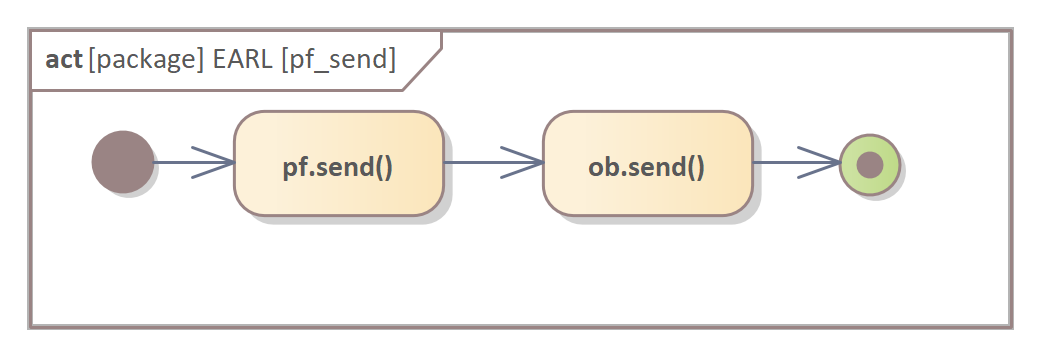
\includegraphics[height=\myheight]{img/basic_earl_model/pf_send.png}} \quad
%		\subfloat[$receive()$\label{fig:pf_receive}]{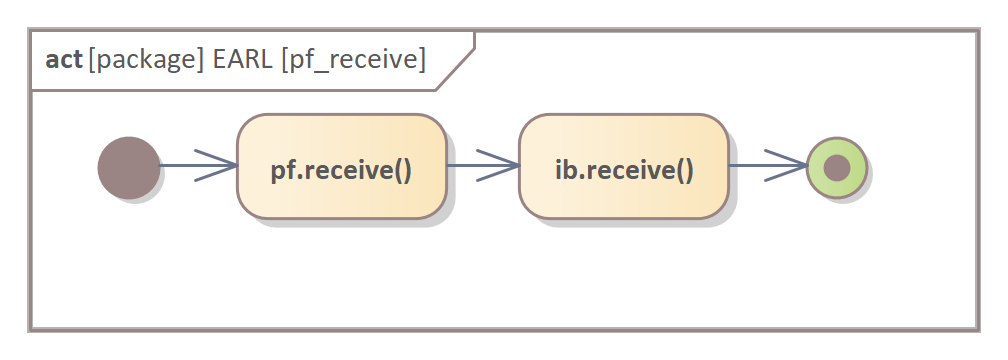
\includegraphics[height=\myheight]{img/basic_earl_model/pf_receive.png}}
%		\caption{\PrimitiveTransitionFunction{} operations}
%		\label{fig:pf_operations}
%	\end{figure}
	


	
	\TerminalConditions{} used by a~\BasicBehaviour{} and \InitialConditions{} utilised within an~\FsmTransition{}
	can be decomposed into \Predicates{}. The~\Predicate{} takes its arguments from \Subsystem{}
	\Buffers{}, see \Figures{}~\ref{fig:warstwa_podsystemu} and~\ref{fig:buffer_usage}. \Predicate{} executes an operation
	called $\fun{}$ producing a~Boolean output. Similarly to \PrimitiveTransitionFunctions{}, \Predicate{} can aggregate other \Predicates{}, with the same no-cycles restriction.
	
	\subsection{\EmbodiedAgent{} Communication}
	\label{sec:communication}
	
	The general system architecture is defined by the \Agents{} and their \Subsystems{}, being the building blocks forming the system structure, and the communication links between those entities.
	In a~way, the architecture is defined by the constraints that are imposed on permissible connections. If no constraints are imposed on the communication links, then the system designer
	has an excessive freedom of choice, which in the case of his limited experience might lead to an obscure structure.
	Therefore, architectures limiting this choice are preferred, thus leading to freedom from choice \cite{dennis2016smartmdsd}. This provides guidance to
	the designers, which results in a~clear system structure.
	
	
	\begin{figure}[h]
		\centering
		\begin{center}
			{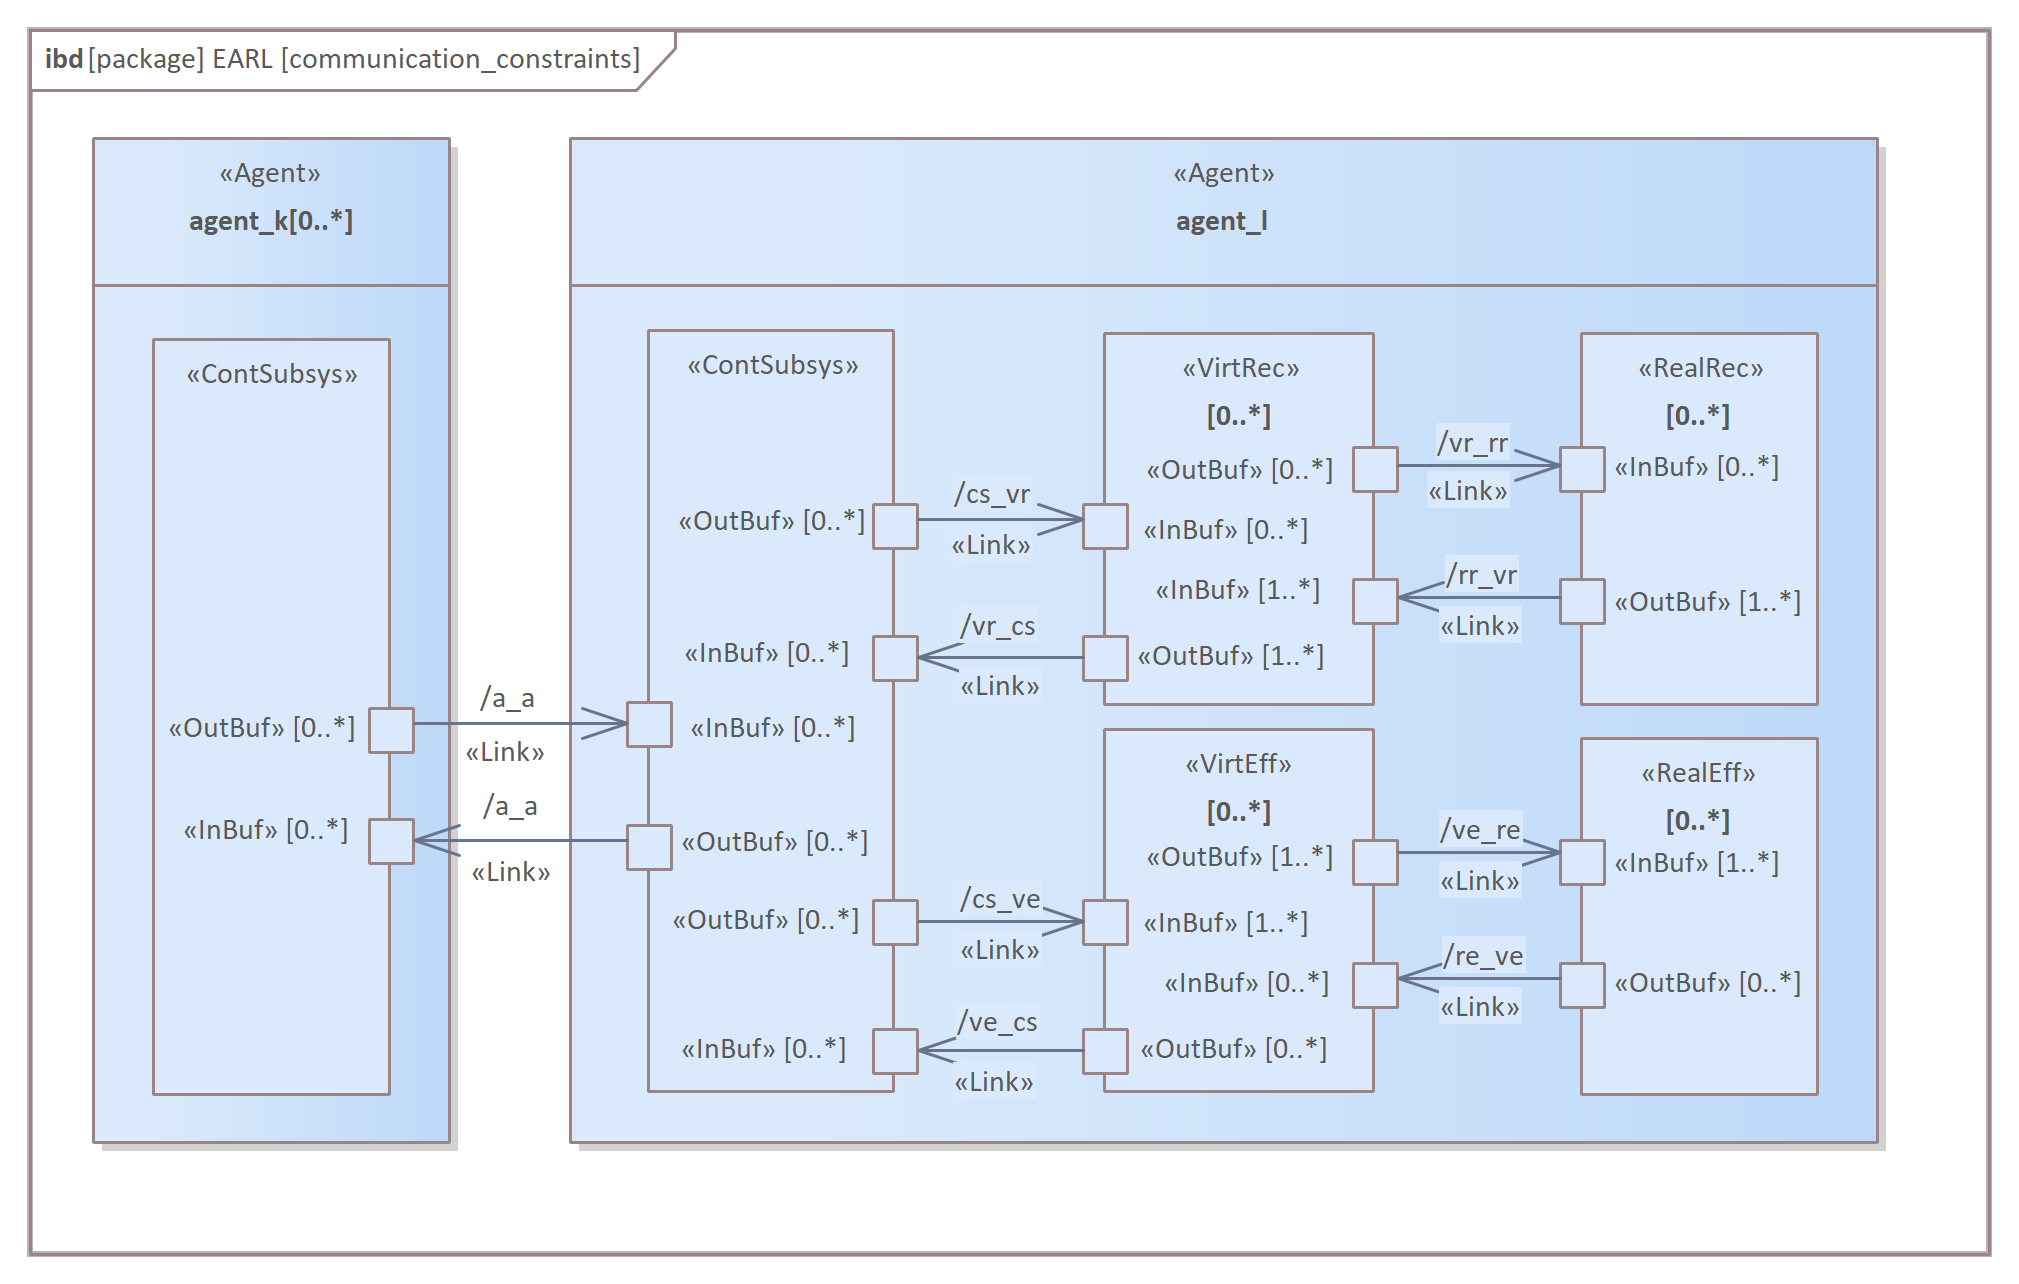
\includegraphics[width=0.95\columnwidth]{img/basic_earl_model/communication_constraints.png}}
		\end{center}
		\caption{Communication constraints, where $agent\_k \neq agent\_l$}
		\label{fig:communication}
	\end{figure}	
	
	In the case of EARL, inter-agent and inter-subsystem communication \cite{Zie:06Springer} is defined by \UnidirectionalCommunicationLinks{} (see \Figures{}~\ref{fig:warstwa_systemu} and~\ref{fig:buffer_usage}).
	The communication takes place between \InputBuffers{} and \OutputBuffers{} of \Subsystems.
	\Figure{}~\ref{fig:communication} presents acceptable communication links between pairs of \Subsystems{}.
	Note that the \InterAgentCommunication{} is realised between the \ControlSubsystems{} of the communicating agents.
	Additionally, \Figure{}~\ref{fig:communication} shows that for each \RealEffector{} present in the system at least one transmission chain should exist.
	The commands produced by the \ControlSubsystem{}, transformed by the \VirtualEffector{}, must reach the \RealEffector{}.
	Analogically, for each \RealReceptor{}, there is one compulsory communication chain that transmits and processes sensory data. The \RealReceptor{} provides data to the
	\VirtualReceptor{} which in an aggregated form passes it to the \ControlSubsystem{}. The other \CommunicationLinks{} appearing in \Figure{}~\ref{fig:communication} are not obligatory.
	To define bidirectional communication, a~pair of \UnidirectionalCommunicationLinks{} is used. Detailed discussion of communication in \EmbodiedAgent{} systems is presented in \cite{hexel-jint2019}.
	
		
	
	\subsection{Types of \Agents{}}\label{sec:agent_types}
	Four general activities of an \Agent{} can be distinguished~\cite{zielinski-kka:2017}:
	\begin{description}
		\item[C] -- overall control of the agent,
		\item[E] -- exerting influence over the environment by using effectors,
		\item[R] -- gathering the information from the environment by using receptors, and
		\item[T] -- inter-agent communication (transmission).
	\end{description}
	
	The first activity is indispensable, but the other three are optional, thus eight types of \Agents{} result (Table~\ref{tab:kinds-of-agents}), depending on their capabilities.
	However, only seven are of utility, as an agent without any of the optional capabilities is useless.
	
	\begin{table}[H]
		\centering
		\caption{Type of \Agent{}, number of its \Subsystems{} ($|\protect\eve{}|$, $|\protect\ere{}|$, $|\protect\evr{}|$, $|\protect\err{}|$) and number of inter agent communication \Links{} ($|\protect\eaa{}|$)
			expressed with respect to the number of \Buffers{} of the considered \Agent{}}
		\scalebox{1.0}{
			\begin{tabular}{c c c c c c c l}
				\toprule
				& \boldmath$|\ecs{}|$ & \boldmath$|\protect\eve{}|$  & \boldmath$|\protect\ere{}|$  & \boldmath$|\protect\evr{}|$ & \boldmath$|\protect\err{}|$ & \boldmath$|\protect\eaa{}|$ & \textbf{Description}\\
				\midrule				
				\textbf{C}    & 1 & 0    & 0    & 0    & 0    & 0    & zombie (useless) \\
				\textbf{CT}   & 1 & 0    & 0    &  0   & 0    & 1..* & purely computational agent\\
				\textbf{CE}   & 1 & 1..* & 1..* &  0   & 0    & 0    & blind agent \\
				\textbf{CR}   & 1 & 0    & 0    & 1..* & 1..* & 0    & monitoring agent\\
				\textbf{CET}  & 1 & 1..* & 1..* &  0   & 0    & 1..* & teleoperated agent \\
				\textbf{CRT}  & 1 & 0    & 0    & 1..* & 1..* & 1..* & remote sensor \\
				\textbf{CER}  & 1 & 1..* & 1..* & 1..* & 1..* & 0    & autonomous agent \\
				\textbf{CERT} & 1 & 1..* & 1..* & 1..* & 1..* & 1..* & full capabilities \\
				\bottomrule
			\end{tabular}
 		}
		\label{tab:kinds-of-agents}
	\end{table}	
	
	
	\subsection{Specification of a~Particular Robot Control System}
	\label{sec:spec-spec}
	
	The particular structure of a~system is specified by application of instances of specialisations of blocks~\cite{Friedenthal:2015} constituting the general model presented above.
	The names of instances should be long enough to be descriptive and intuitive to interpret, thus reducing the need for additional glossaries.
	In our approach, each instance can set the number of parts and references (e.g., associated \Buffers{}), however, within the limits imposed by the general model.
	Similarly, each instance can redefine the particular operations of parent blocks present in the general model (e.g., each instance of \PrimitiveTransitionFunction{}
	redefines $\epf{}.execute$ operation).
	
	In general, a~system instance is defined as a~graph. Its nodes represent \Agents{}~$\ea{}$ and the directed arcs represent the communication \Links{}~$\eaa{}$ between them.
	It is a~good practice to name \Links{} by using the names of communicating \Agents{}: first the source \Agent{} name, then a~underscore, and finally the destination \Agent{} name.
	\InputBuffers{} and \OutputBuffers{} of the \ControlSubsystems{} are depicted as sources and destinations of \ValueTypes{} being transmitted through the \Links{}.
	The \Buffer{} names reflect the content of \ValueType{} being transmitted. The \Subsystems{} are defined analogically.
	
	Specification refers to a~system with a~static structure and invariable behaviour, or a~system with a~variable structure at a~certain time instant. To specify a~particular system, instances of the relevant concepts appearing in the general system model should be concretised. The \SysML{} diagrams~\cite{systems7020019} are a~part of
	the \EARL{}-based system. Some of the \EARL{} concepts are specified mathematically:
	\begin{itemize}
		\item model and system instance constraints that can not be practically formulated in diagrams,
		\item $\fun{}$ operations of \Predicates{}, and
		\item some calculations performed inside actions of \Activity{} \Diagrams{} of \PrimitiveTransitionFunctions{}, e.g.,\ control laws.
	\end{itemize}
	In addition, mathematical notation is used to express formal conditions ascertaining the correctness of the composition of \PrimitiveTransitionFunctions{}.
	

	\section{Example of a~System Specified Using \EARL}
	\label{sec:example}
	This section is devoted to the illustration of how to use the \EARL{} language to specify a~robot control system. The example presents a~single robot multi-agent system
	containing \textbf{CT} and \textbf{CET} agents. For the obvious reason of briefness, this description is not a~complete specification, but contains only examples of
	important aspects of the general model and its use:
	\begin{itemize}
		\item General system use cases.
		\item Structure of the whole \System{} with \Buffers{}, \InternalMemories{}, \InterAgentCommunicationLinks{}, and \ValueTypes{} used by them.
		\item Structure of the particular \Agent{} with \Buffers, \InternalMemories{}, \InterSubsystemCommunicationLinks{}, and \ValueTypes{} used by them.
		\item Specification of a~particular \Subsystem{}, its structure and behaviour, i.e., \Buffers{}, \InternalMemories{},\TransitionFunctionCompositionVariables{}, \ValueTypes{}, \Fsm{}, \BasicBehaviours{} and their
		\TerminalConditions{} and \ErrorConditions{}; \Predicates{}, \FsmTransitions{} and their \InitialConditions{}; method of both composition and execution
		of \PrimitiveTransitionFunctions{} and control law utilised in the activity diagram of \PrimitiveTransitionFunction{}. \PrimitiveTransitionFunctions{} can be mapped into the \SysML{} activities.
	\end{itemize}
	
	A~manipulation robot with N degrees of freedom and a~gripper is considered, capable to perform e.g. pick and place task. The specification process starts with the definition of the \System{} structure.
	Tips on the specification of requirements and use cases using \SysML{} can be found in~\cite{requc1,requc2}.
	
	
	\subsection{System use cases}
	Diagram~\ref{fig:system_use_cases} illustrates general system use cases. The User can request the robot to:
	\begin{itemize}
		\item Synchronize the robot's drives,
		\item Perform the movement in joint or operational space,
		\item Perform the emergency stop action, or
		\item Perform Pick and Place task, which is composed of the movement in joint and operational space, and in certain conditions can be ended by the emergency stop action.
	\end{itemize}
	\begin{figure}[H]
		\centering
		\begin{center}
			{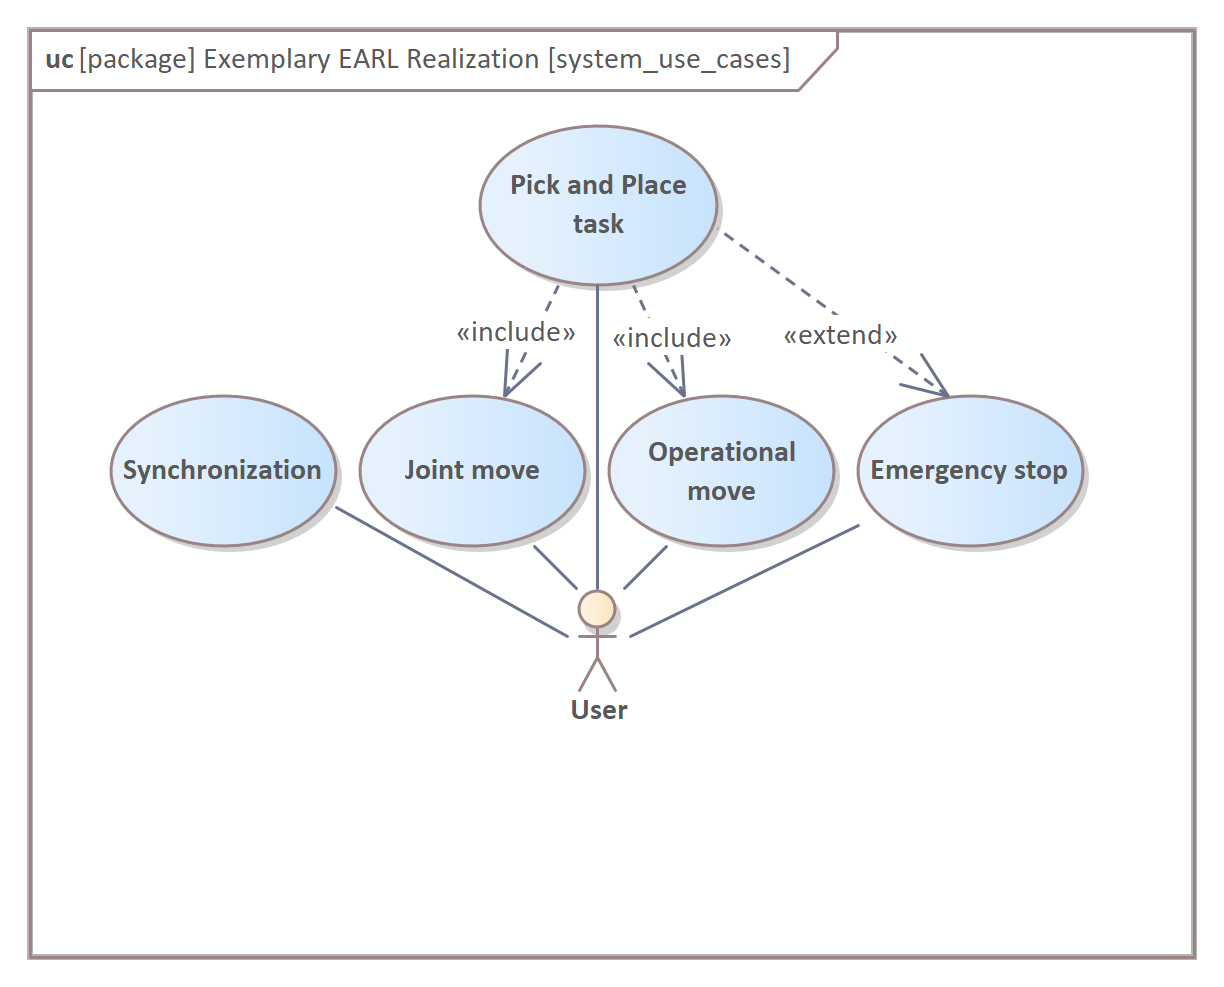
\includegraphics[width=0.6\columnwidth]{img/basic_earl_instance/system_use_cases.png}}
		\end{center}
		\caption{System use cases}
		\label{fig:system_use_cases}
	\end{figure}
	
	\subsection{Structure of the~\System{} Composed of \Agents{}}
	Diagram~\ref{fig:value_types_pkgs} illustrates structure of Value Types and Units packages used in the presented~\System{}.
	\begin{figure}[H]
		\centering
		\begin{center}
			{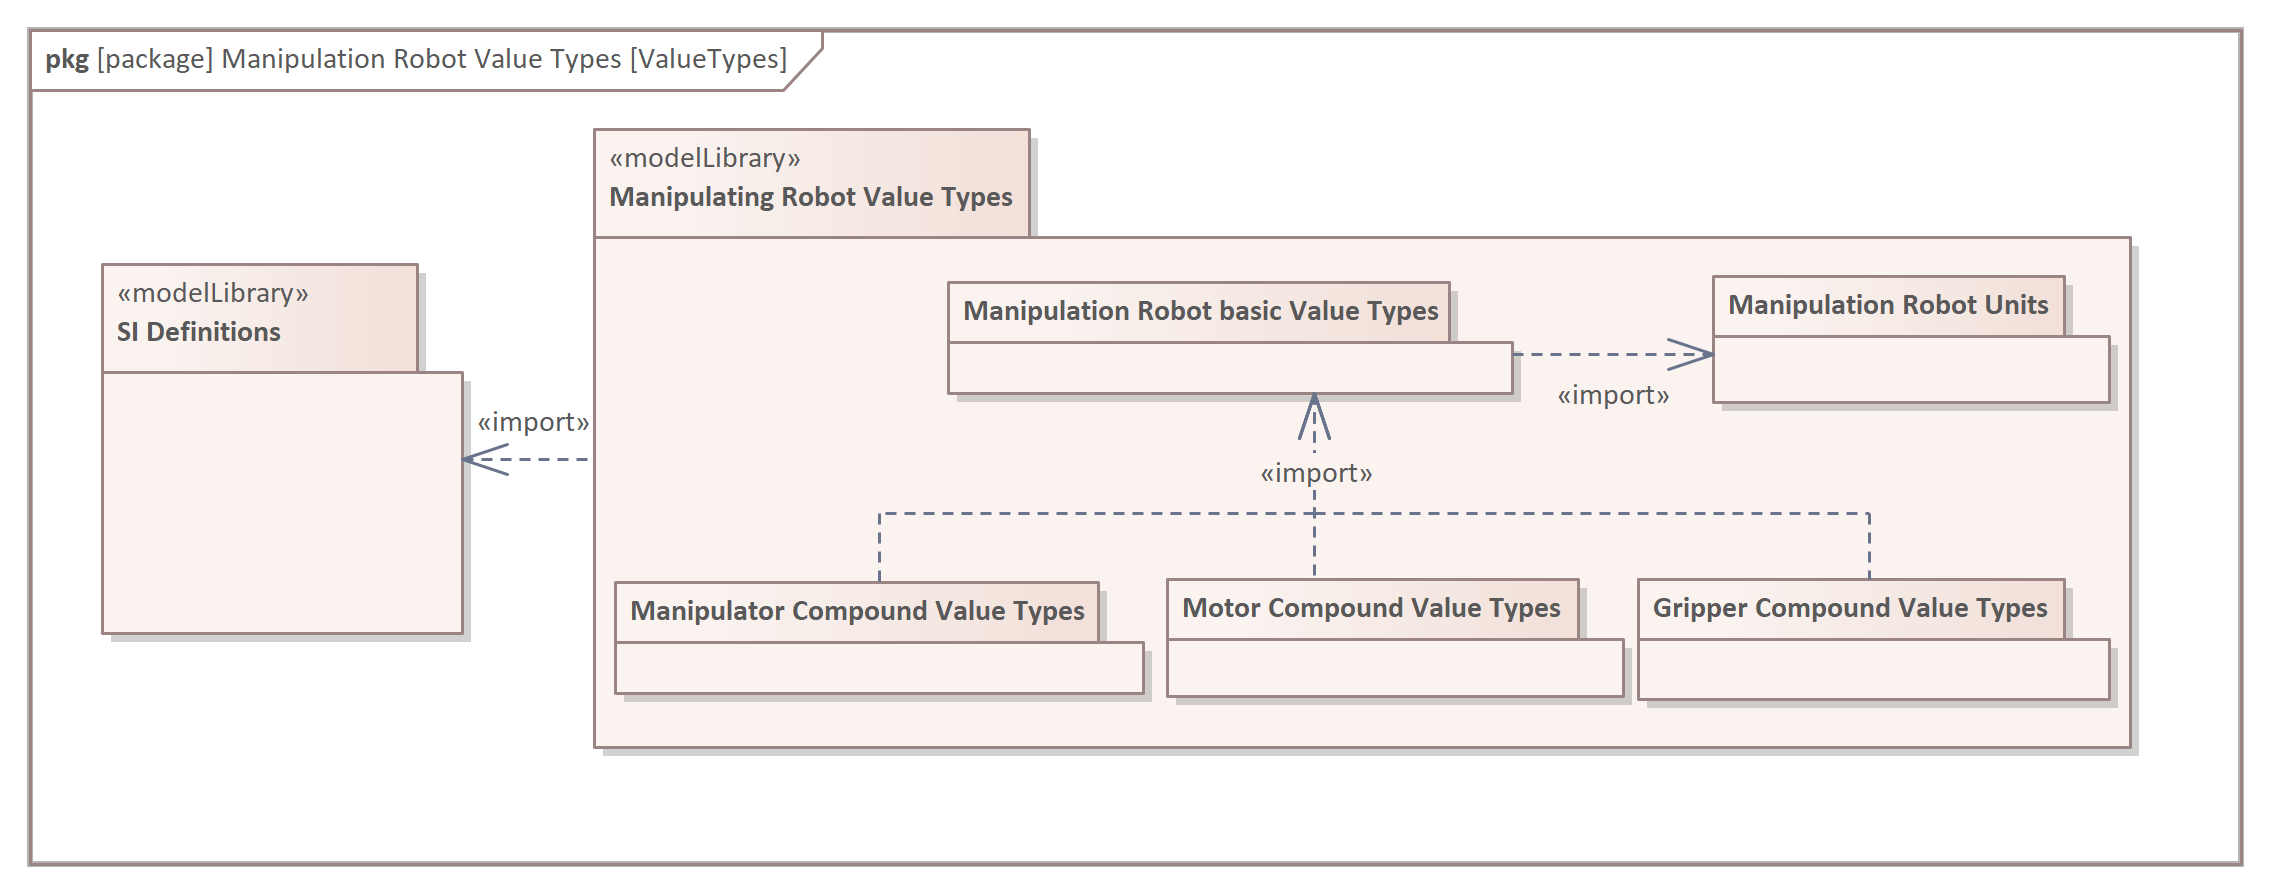
\includegraphics[width=\columnwidth]{img/value_types/value_types_pkgs.png}}
		\end{center}
		\caption{Value Types and Units packages structure}
		\label{fig:value_types_pkgs}
	\end{figure}

	Diagram~\ref{fig:units} presents Units definitions, while diagram~\ref{fig:basic_value_types} illustrates basic Value Types used in the Compound Value Types definitions.

	\begin{figure}[H]
	\centering
	\begin{center}
		{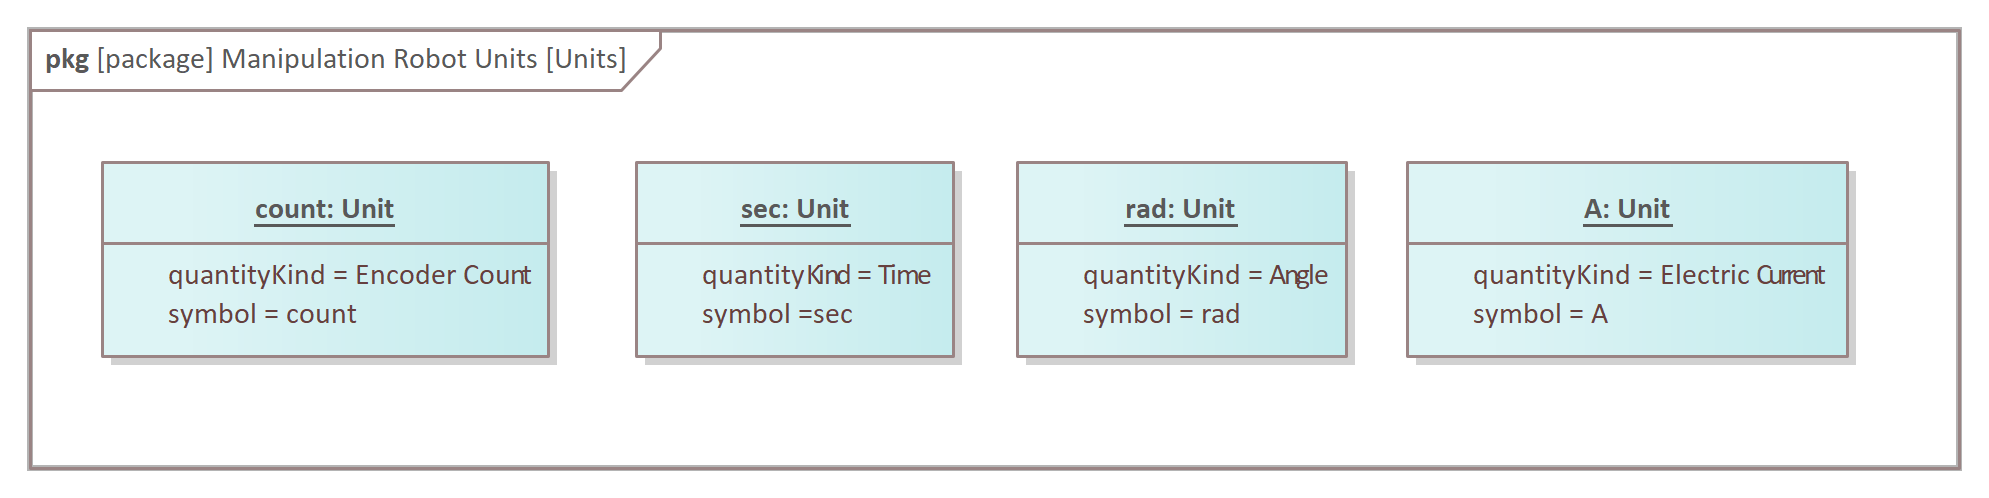
\includegraphics[width=\columnwidth]{img/value_types/units.png}}
	\end{center}
	\caption{Units definitions}
	\label{fig:units}
	\end{figure}

	\begin{figure}[H]
	\centering
	\begin{center}
		{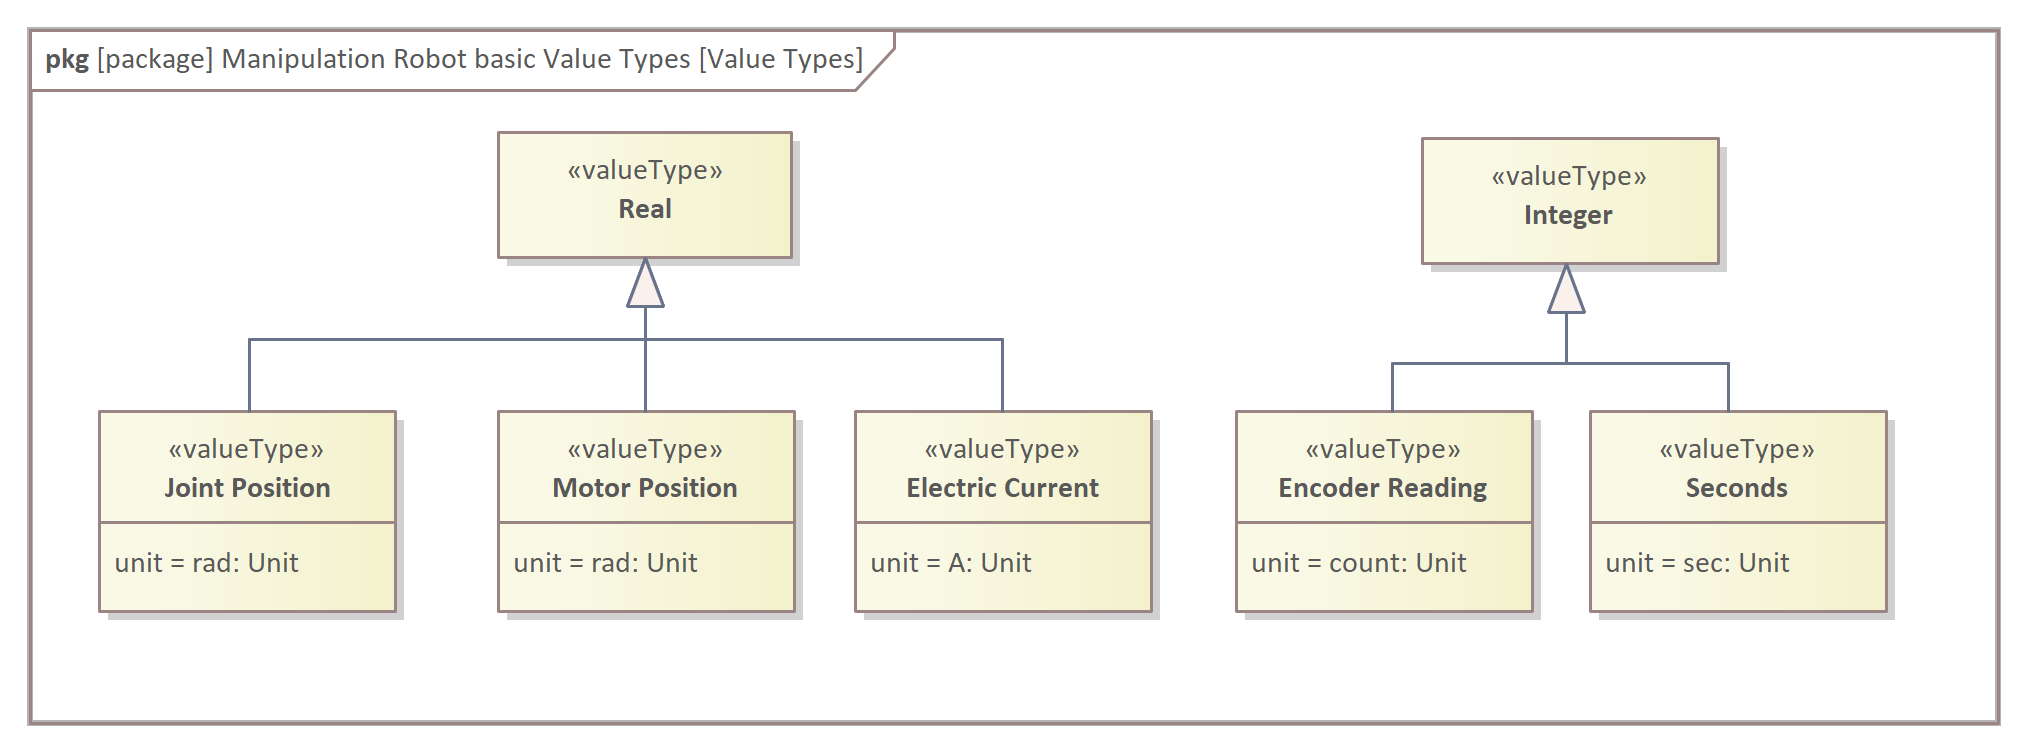
\includegraphics[width=\columnwidth]{img/value_types/basic_value_types.png}}
	\end{center}
	\caption{Basic Value Types definitions}
	\label{fig:basic_value_types}
	\end{figure}
	
	There are three \Agents{} in the \System{} (\Figure{}~\ref{fig:all_agents}).
	The \Agent{} $\ea{task}$ supervises the task execution, i.e.,\ picking and placing objects; the \Agent{} $\ea{manip}$ controls the N-DOF manipulator; and the \Agent{}
	$\ea{grip}$ controls the gripper. The gripper controller is separate from the manipulator controller, because different grippers can be attached to the manipulator, thus separate
	\Agents{} facilitate system~modification. Both $\ea{manip}$ and $\ea{grip}$ are aggregated in \GroupofAgents{} $\ega{arm}$. Figure~\ref{fig:all_agents_blocks_instances} shows alternative representation of the exemplary \System{} -- in this case full names of blocks were depicted.
	
	\begin{figure}[H]
		\centering
		\begin{center}
			{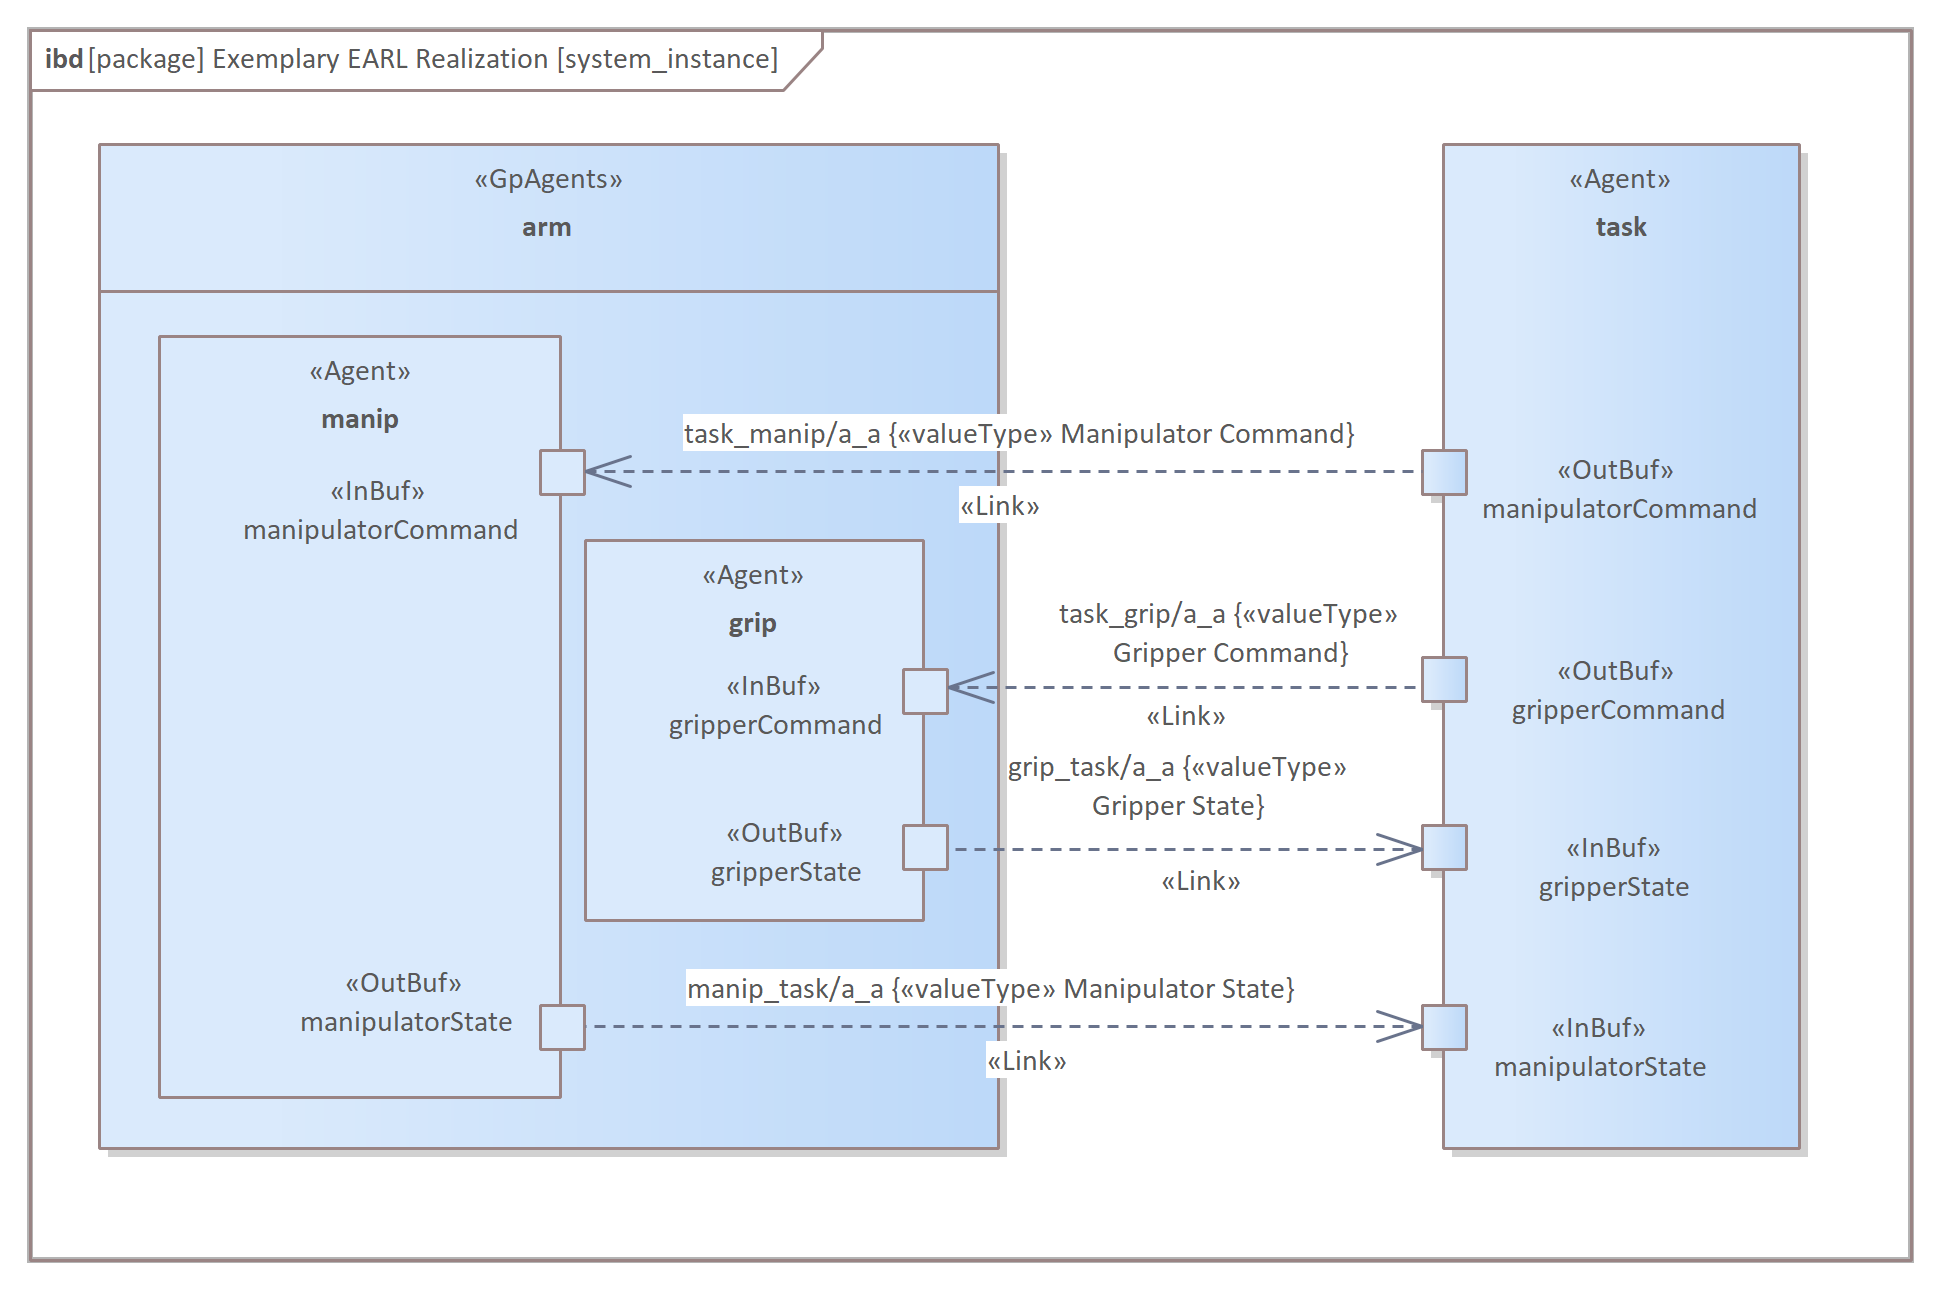
\includegraphics[width=.9\columnwidth]{img/basic_earl_instance/system_instance.png}}
		\end{center}
		\caption{Structure of the considered exemplary \System{}}
		\label{fig:all_agents}
	\end{figure}
	
	
	
	\begin{figure}[H]
	\centering
	\begin{center}
		{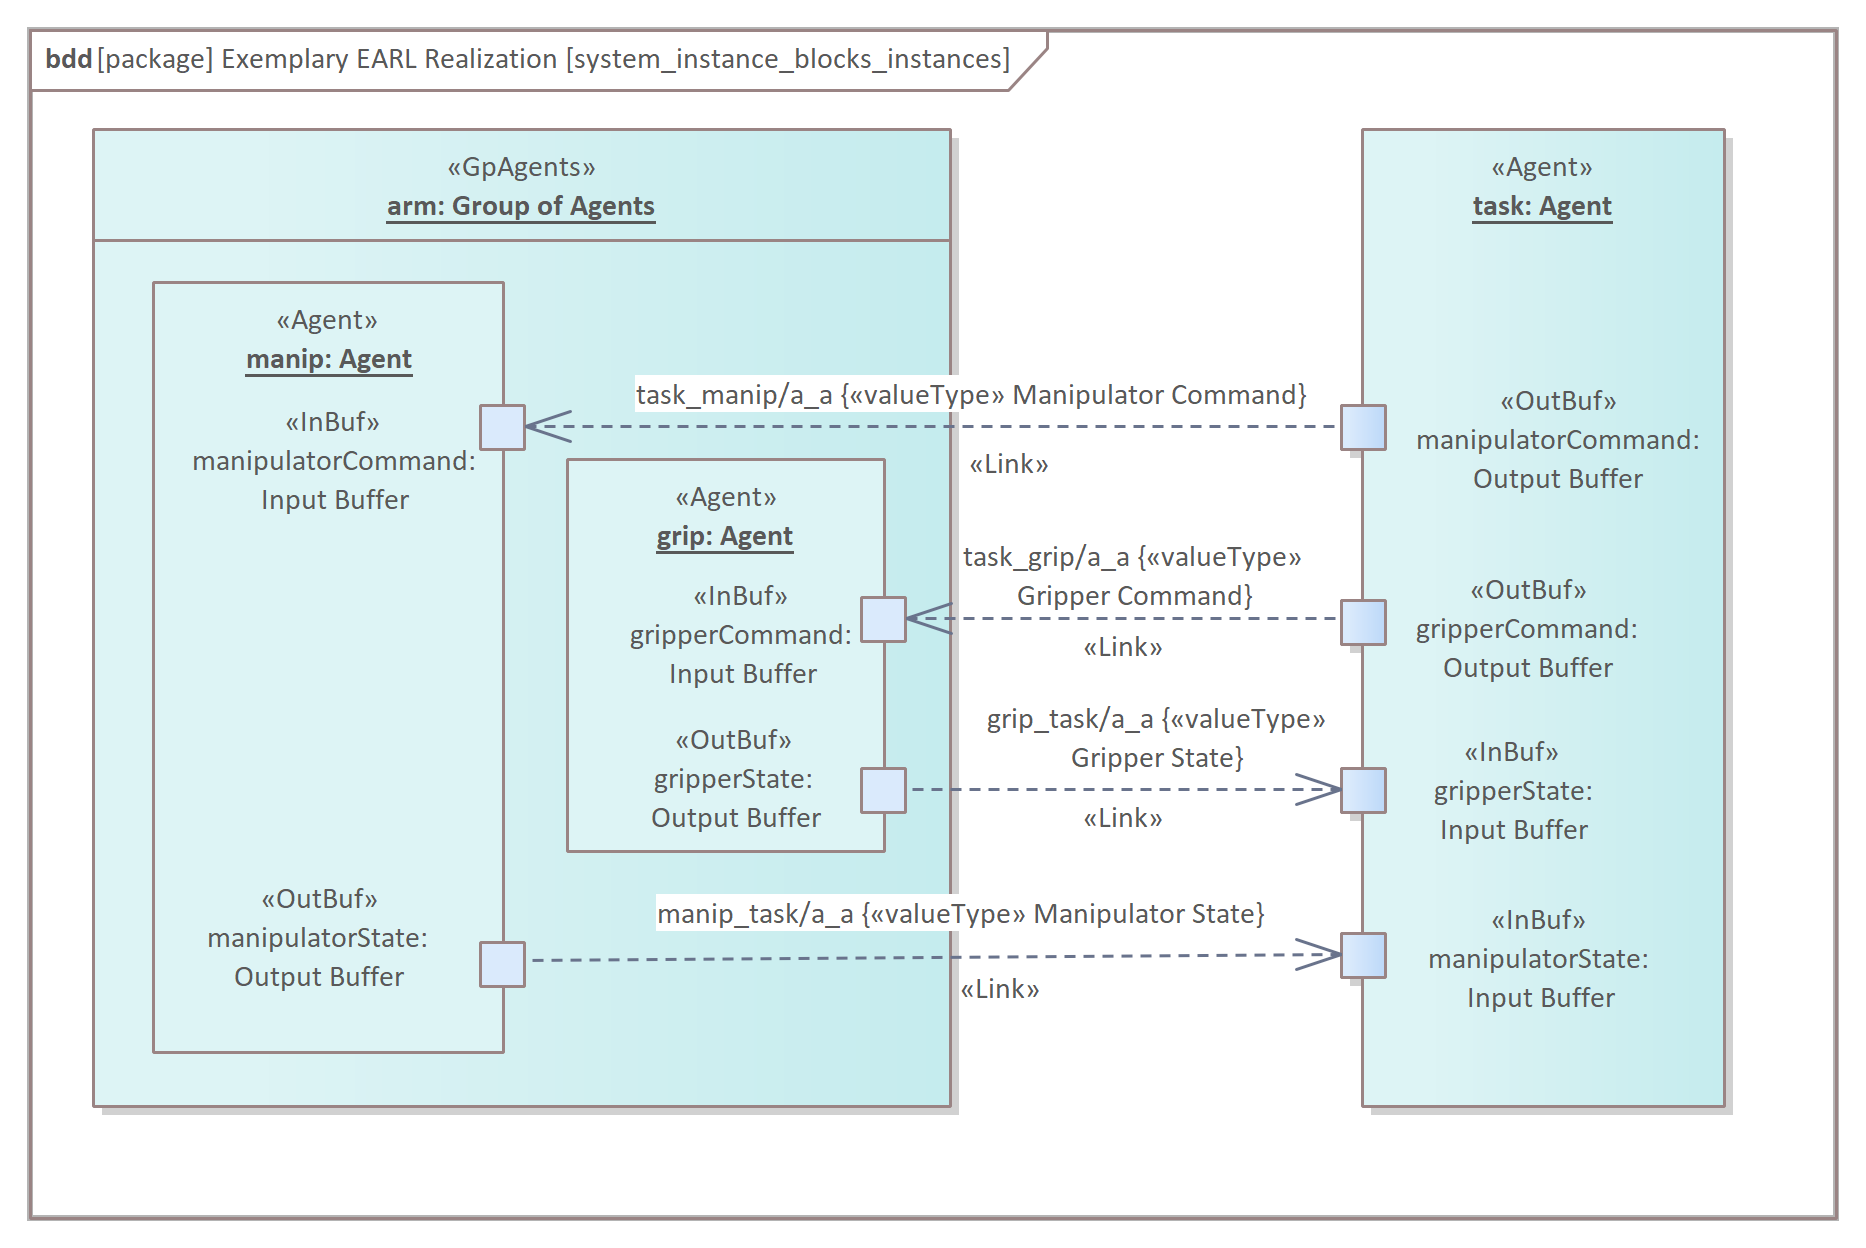
\includegraphics[width=.9\columnwidth]{img/basic_earl_instance/system_instance_blocks_instances.png}}
	\end{center}
	\caption{Structure of the considered exemplary \System{} (full blocks names)}
	\label{fig:all_agents_blocks_instances}
\end{figure}	
	
	
	
	\Figure{}~\ref{fig:sys_messages} presents the \ValueTypes{} transmitted between the \Agents{}. The \TaskAgent{} $\ea{task}$ sends Manipulator Commands to the
	\ManipulatorAgent{} $\ea{manip}$. The commands contain parameters, e.g.,\ operational or joint position setpoints and a~command to perform emergency stop.
	In return $\ea{task}$ gets a~Manipulator State \ValueType{} containing: the current operational or joint position, status of the manipulator movement and information
	whether an emergency stop occurred.
	The \TaskAgent{} $\ea{task}$ sends Gripper Command messages to the \GripperAgent{}~$\ea{grip}$ and receives Gripper Status in return.
	Similarly to messages exchanged between $\ea{manip}$ and $\ea{task}$ \Agents, the Gripper Command and Gripper Status messages contain parameters describing
	the desired and current gripper finger~positions. Both $\ea{manip}$ and $\ea{grip}$ are aggregated in \GroupofAgents{} $\ega{arm}$.
	
	\begin{figure}[H]
		\centering
		\begin{center}
			{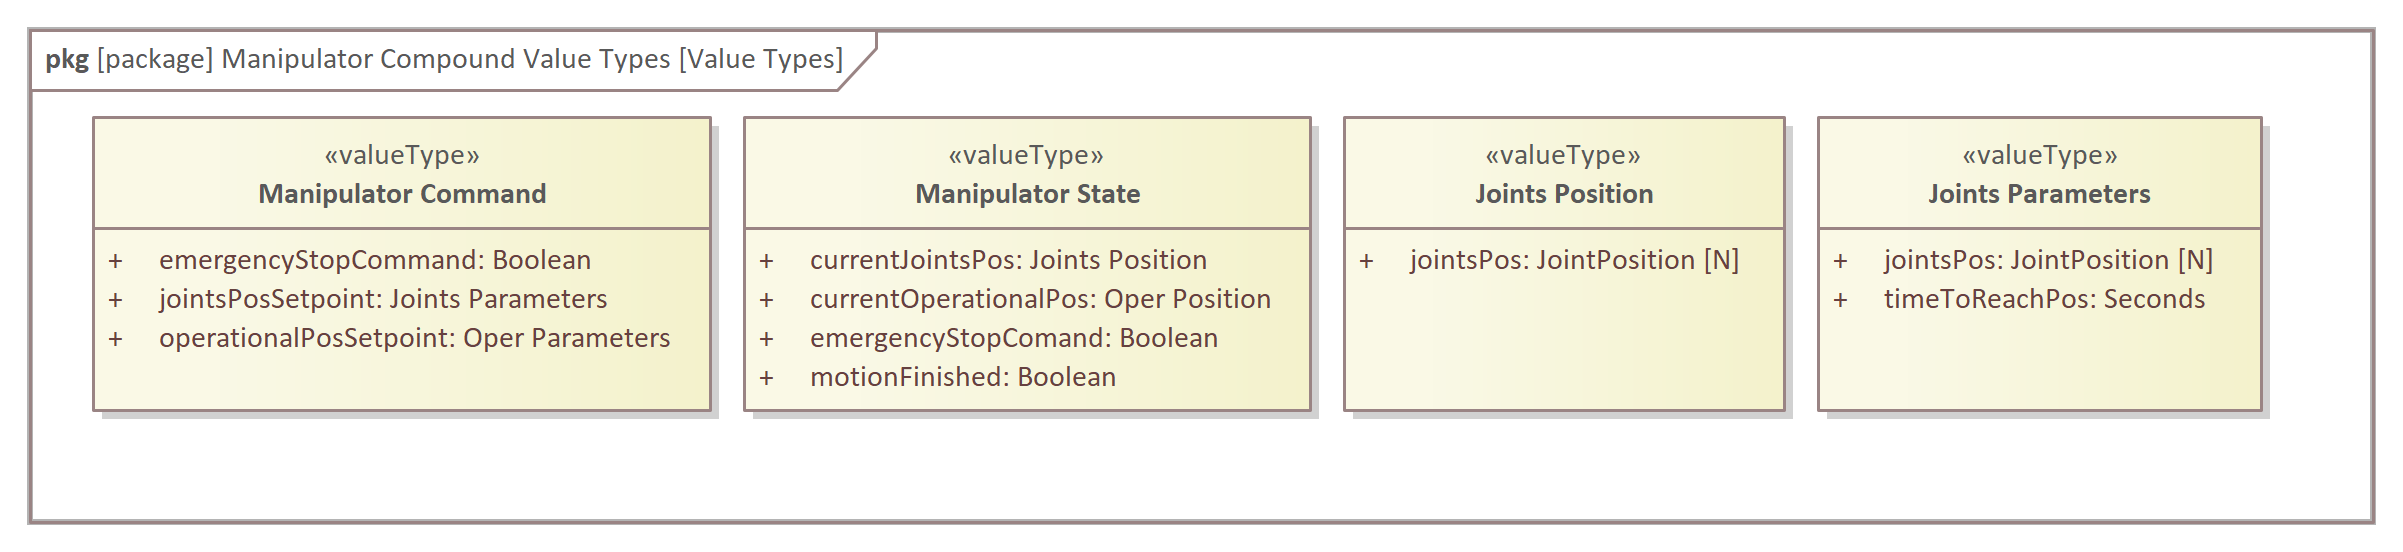
\includegraphics[width=\columnwidth]{img/value_types/manipulator_compound_value_types.png}}
		\end{center}
		\caption{\ValueTypes{} transmitted within the system}
		\label{fig:sys_messages}
	\end{figure}
	
	\subsection{\ManipulatorAgent{} $manip/a$}
	
	The structure of the \ManipulatorAgent{} $\ea{manip}$ is presented in \Figure{}~\ref{fig:a_m}.
	Each \RealEffector{} $\ere{}$ represents one of the $N$ drives of manipulator joints.
	Each drive is controlled by a~\VirtualEffector{} that, e.g., implements a~motor position regulator.
	All $N$ \VirtualEffectors{} $\eve{}$ are controlled by a~single \ControlSubsystem{} $\ecs{}$, which causes the manipulator to move either in joint space,
	where it interpolates between joint positions, or in operational space, where it interpolates between Cartesian poses of a~frame affixed to a~chosen link of the kinematic chain. Both \VirtualEffectors{} and \RealEffector{} are aggregated in \GroupofSubsystems{} $\egs{motors}$.
	\begin{figure}[H]
		\centering
		\begin{center}
			{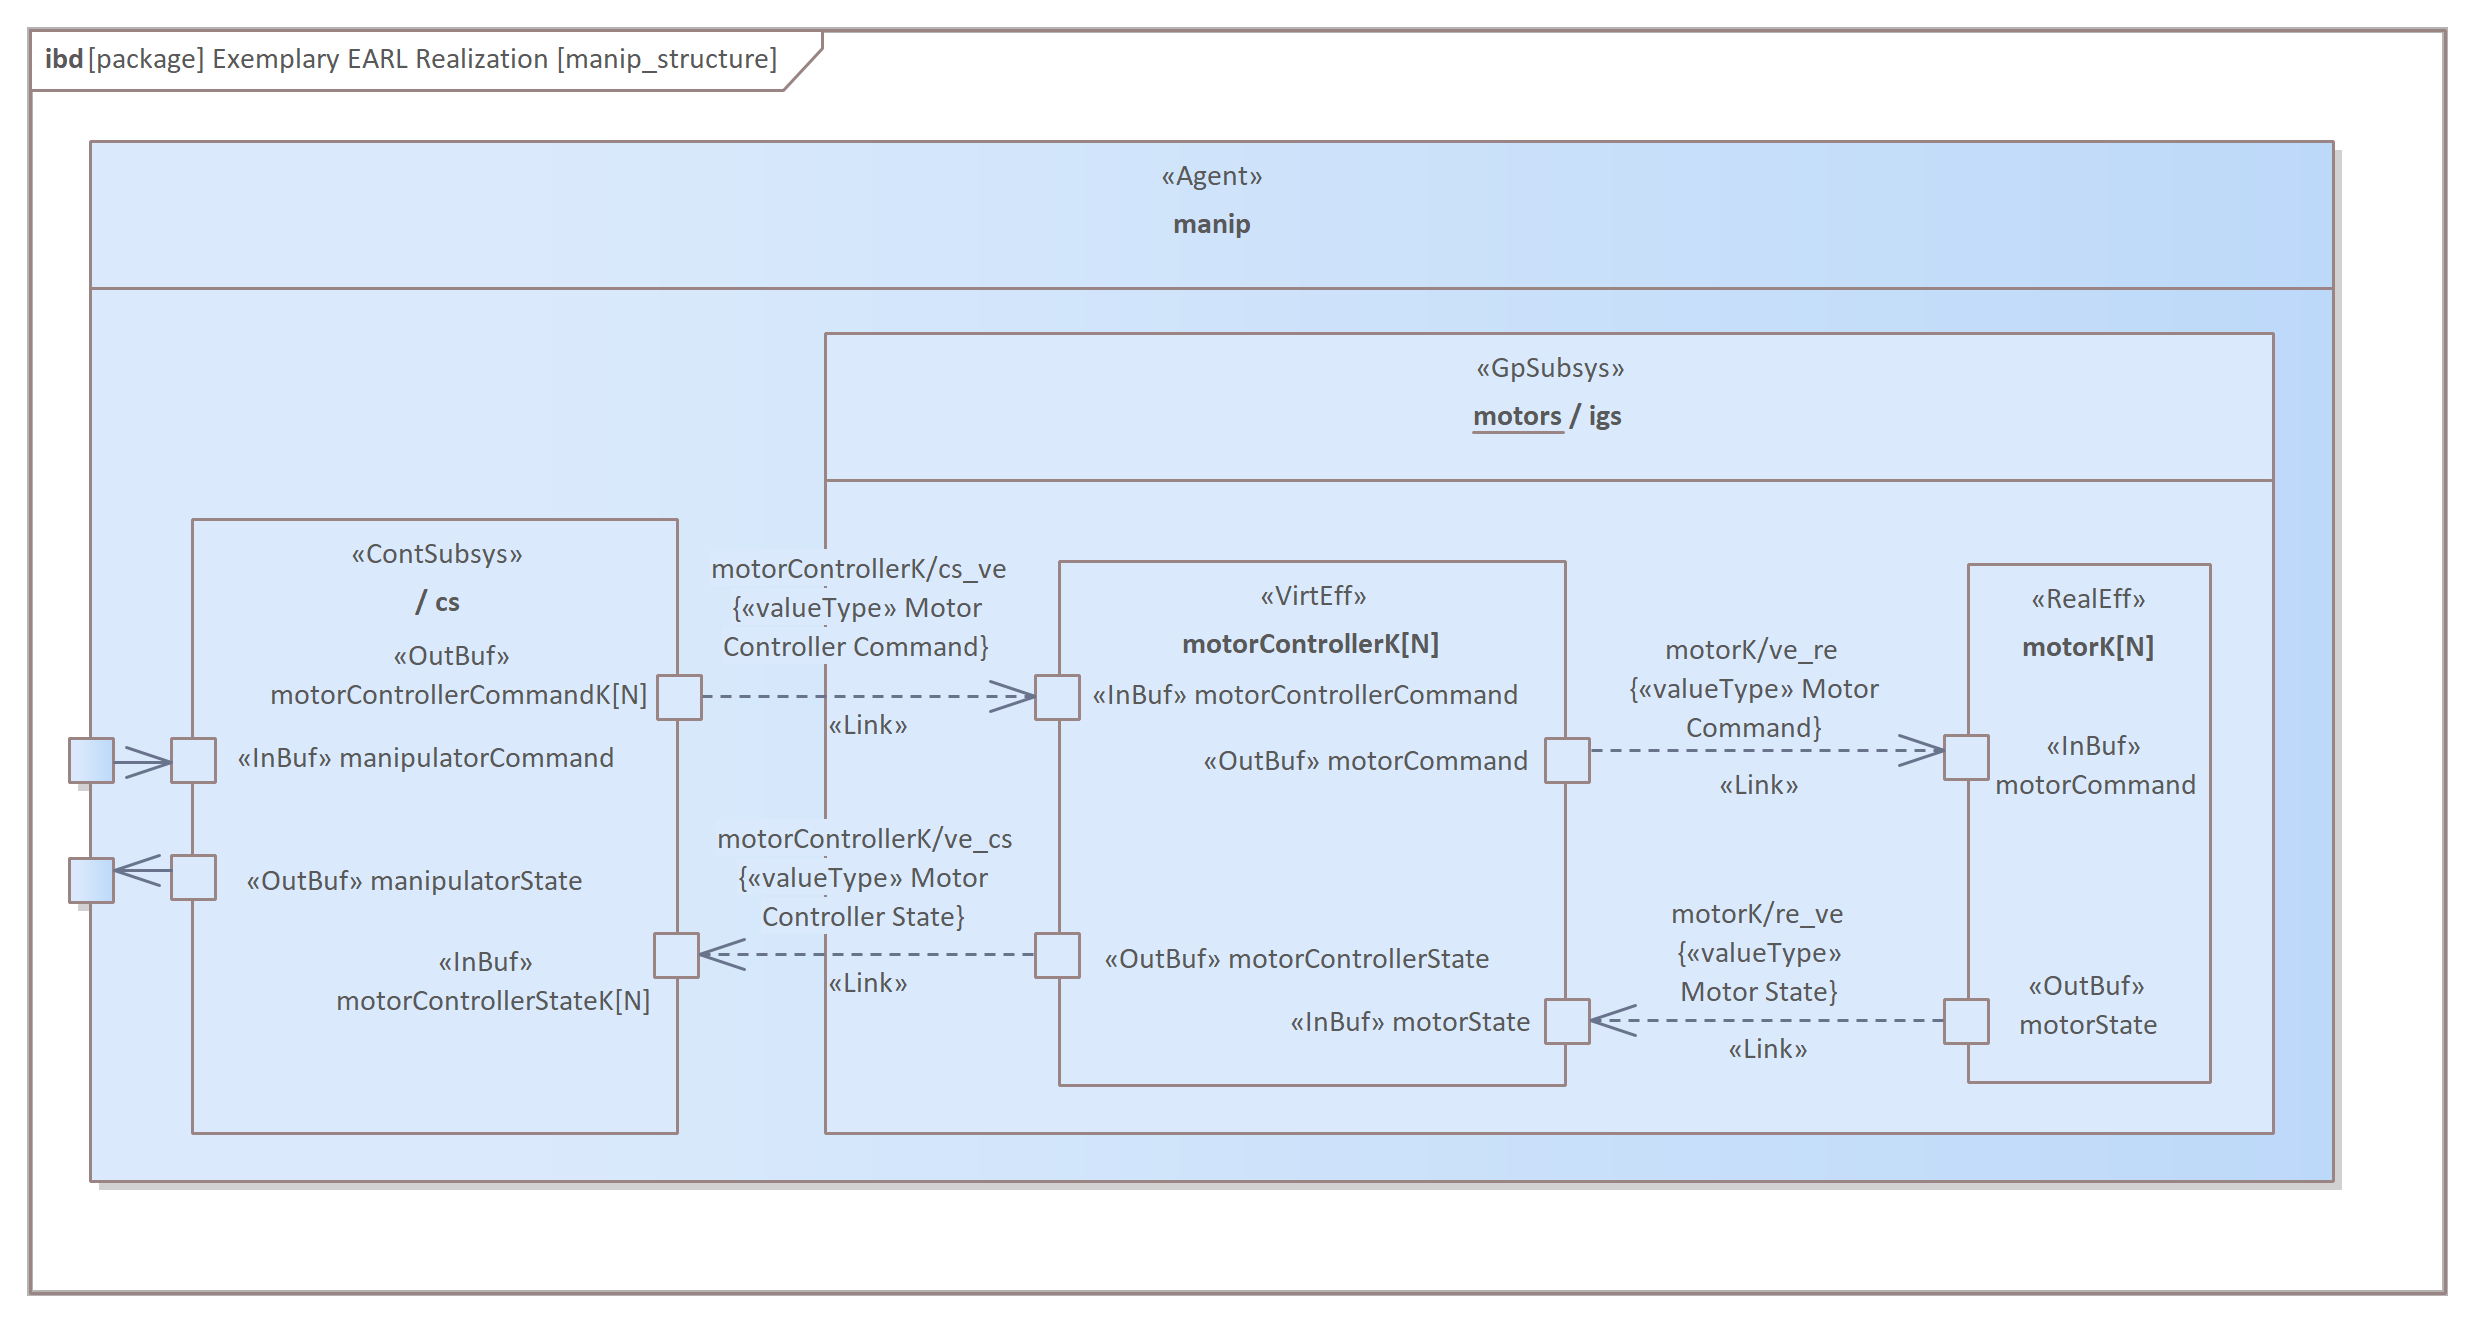
\includegraphics[width=\columnwidth]{img/basic_earl_instance/manip_structure.png}}
		\end{center}
		\caption{Structure of the \Agent{} $\protect\ea{manip}$; letter K placed at the end of the instance name should be substituted by a~number, i.e.\ $K\in\{1,...,N\}$}
		\label{fig:a_m}
	\end{figure}
	
	The \ValueTypes{} transmitted inside the \ManipulatorAgent{}~$\ea{manip}$ are presented in \Figure{}~\ref{fig:a_manip_messages}.
	The~\ControlSubsystem{} $\ecs{}$ sends MotorControllerCommand to each \VirtualEffector{}\\ $\eve{motorControllerK}$. The~\ValueType{} contains the desired winding current
	value or a~command to switch the hardware driver to the emergency stop state. Each \VirtualEffector{} $\eve{motorControllerK}$ sends to
	the \ControlSubsystem{} $\ecs{}$ information about the current motor position and whether the hardware driver is in an emergency stop state.
	Each \VirtualEffector{} $\eve{motorControllerK}$ sends the desired motor winding current to its respective \RealEffector{} $\ere{motorK}$, and in return receives the encoder readings.
	\Table{}~\ref{tab:am-cs-mb} describes types of data utilized in the $\ea{manip}.\ecs{}$.
	
	\begin{figure}[H]
		\centering
		\begin{center}
			{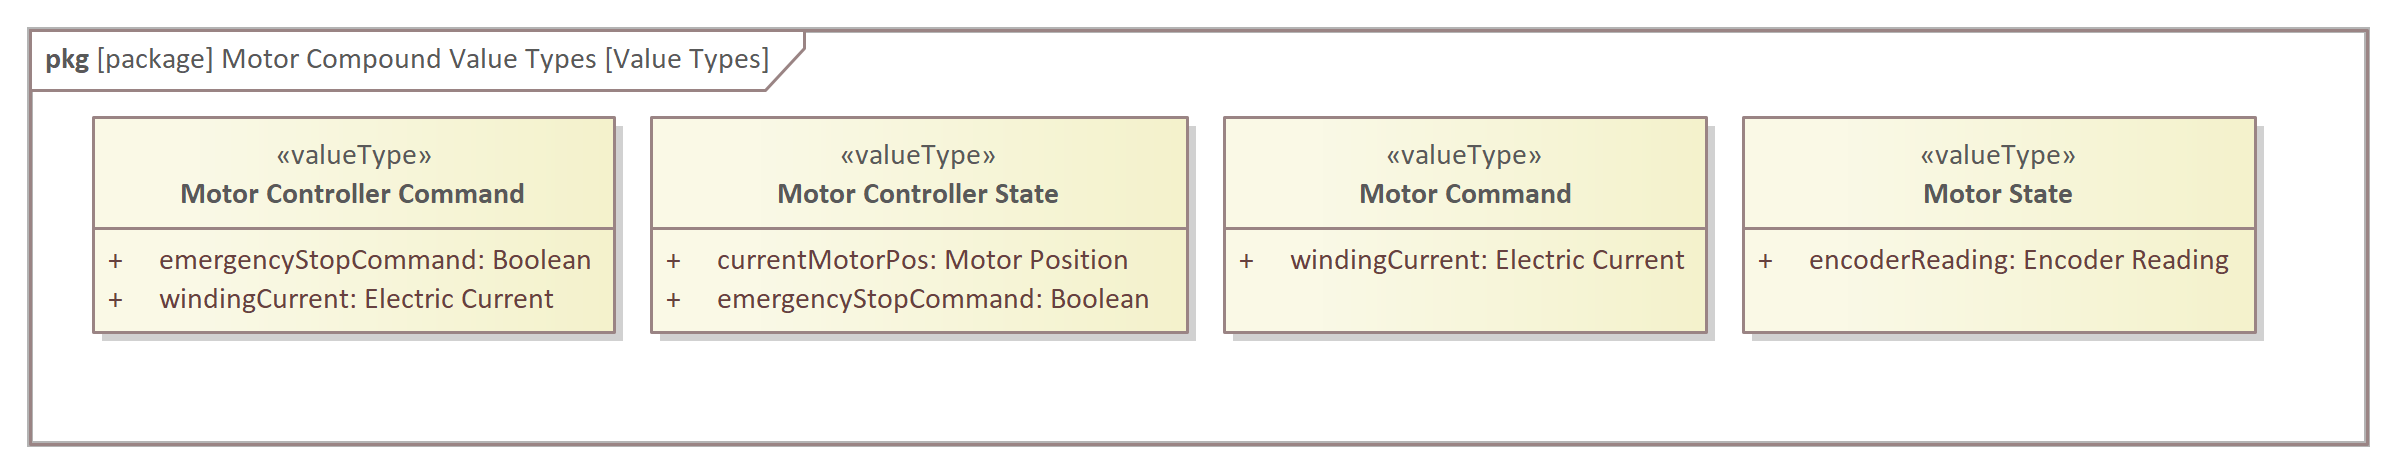
\includegraphics[width=\columnwidth]{img/value_types/motor_compound_value_types.png}}
		\end{center}
		\caption{Definition of $\protect\ea{manip}$ \ValueTypes{}}
		\label{fig:a_manip_messages}
	\end{figure}
	
	
	
	\begin{table}[H]
		\centering
		\caption{$\protect\ea{manip}.\protect\ecs{}$ \ValueTypes{}}
		\begin{tabular}[]{p{5.0cm} p{2.5cm}}
			\toprule
			\multicolumn{1}{c}{}	& \multicolumn{1}{c}{\textbf{valueType}{}} \\ 
			\midrule
			$\emb{motionFinished}$ & Boolean\\ 
			$\ecv{motionFinished}$ & Boolean\\ 
			$\ecv{currentOperationalPos}$ & Oper Position\\ 
			$\ecv{currentJointsPos}$ & Joints Position\\ 
			$\ecv{emergencyStopCommandK}$ & Boolean\\ 
			$\ecv{windingCurrentK}$ & Real\\ 
			\bottomrule
		\end{tabular}
		\label{tab:am-cs-mb}
	\end{table}	
	
	\Table{}~\ref{tab:am-cs-p} describes \Predicates{} $\ep{}$ used in the \ControlSubsystem{} $\ea{manip}.\ecs{}$. They take as arguments the contents of the buffers and memory.
	The~$newData(\InputBuffer{}.\emsg{})$ function producing Boolean values, returns TRUE if there is new data in the \InputBuffer{}, and FALSE if the data is obsolete.
	
	\begin{table}[H]
		\centering
		\caption{Definitions of $\protect\ea{manip}.\protect\ecs{}.\protect\bp{}.\protect\bfun{}$}
		\begin{tabular}[]{p{3.5cm} p{11.5cm}}
			\toprule
			\multicolumn{1}{c}{$/\bp{}$}	& \multicolumn{1}{c}{$\bfun{}$} \\ 
			\midrule
			$emergencyStop$ & \centered{$\eib{manipulatorCommand}.\emsg{}.emergencyStopCommand \: \lor$\\ $\eib{motorControllerState1}.\emsg{}.emergencyStopCommand \lor \ldots \lor$\\ $\eib{motorControllerStateN}.\emsg{}.emergencyStopCommand$}\\ 
			$motionFinished$& \centered{$\emi{motionFinished}.\emsg{}$}\\ 
			$newJointsPos$ & \centered{$newData(\eib{manipulatorCommand}.\emsg{}.jointsPosSetpoint)$}\\ 
			$newOperationalPos$ & \centered{$newData(\eib{manipulatorCommand}.msg.operationalPosSetpoint)$}\\ 
			$true$ & \centered{TRUE}\\ 
			$false$ & \centered{FALSE}\\ 
			\bottomrule
		\end{tabular}
		\label{tab:am-cs-p}
	\end{table}	
	
	\Tables{}~\ref{tab:am-cs-fsm-t},~\ref{tab:am-cs-bb-tc-ec} describe the \Predicates{} utilised by $\ea{manip}.\ecs{}$.
	\Figure{}~\ref{fig:state_machines_a_m} shows possible transitions between the \FsmStates{} of the \ControlSubsystem{} $\ea{manip}.\ecs{}$ as well as the
	association of \BasicBehaviours{} to particular \FsmStates{}.
	
	\begin{table}[H]
		\centering
		\caption{Initial conditions labelling $\protect\ea{manip}.\protect\ecs{}.\protect\efsm{}$ transitions. It is assumed that
			$\protect\ea{task}$ can not set simultaneously a~new joint position and an operational space pose}
		\small
		\begin{tabular}[]{p{1cm} p{4cm} p{8.0cm} }		
			\noalign{\hrule height 1.0pt} 
			
			\multicolumn{3}{c}{} \\[-2ex]
			
			
			\multicolumn{3}{c}{\textbf{Labels of transitions between \FsmStates}} \\
			
			\multicolumn{3}{c}{ } \\ [-2ex]
			
			
			\multicolumn{3}{c}{ $\ecs{}.\efsm{}.\bt{}.\eic{}.\fun{} \triangleq \textbf{PREDICATE}$} \\ 
			
			\multicolumn{3}{c}{ } \\ [-2ex]
			
			\multicolumn{2}{c}{\makecell{$\bt{}$}} & \makecell{\textbf{PREDICATE}} \\ 
			\hline
			\multicolumn{3}{c}{ } \\ [-2ex]
			
			\multicolumn{2}{c}{$\ent{idle\_jointMove}$} & \centered{$\neg \ep{errTran}.fun() \: \land \ep{newJointsPos}.\fun{}$}  \\ 
			\multicolumn{3}{c}{ } \\ [-2ex]
			
			\multicolumn{2}{c}{$\ent{jointMove\_jointMove}$} & \centered{$\neg \ep{errTran}.fun() \: \land \ep{newJointsPos}.\fun{}$}  \\
			\multicolumn{3}{c}{ } \\ [-2ex]
			
			\multicolumn{2}{c}{$\ent{idle\_operationalMove}$} & \centered{$\neg \ep{errTran}.fun() \: \land \ep{newOperationalPos}.\fun{}$}  \\
			\multicolumn{3}{c}{ } \\ [-2ex]
			
			\multicolumn{2}{c}{$\ent{operationalMove\_operationalMove}$} & \centered{$\neg \ep{errTran}.fun()\: \land \ep{newOperationalPos}.\fun{}$}  \\
			
			\multicolumn{3}{c}{ } \\ [-2ex]
			
			\multicolumn{2}{c}{$\ent{jointMove\_idle}$} & \centered{$\neg\ep{errTran}.fun()$}  \\  
			
			\multicolumn{3}{c}{ } \\ [-2ex]
			
			\multicolumn{2}{c}{$\ent{operationalMove\_idle}$} & \centered{$\neg\ep{errTran}.fun()$}  \\ 
			
			\multicolumn{3}{c}{ } \\ [-2ex]
			
			\multicolumn{2}{c}{$\eet{i\_emergencyStop}$, $i \neq emergencyStop$} & \centered{$\ep{errTran}.fun()$} \\
				
			\noalign{\hrule height 1.0pt} 
		\end{tabular}
		\label{tab:am-cs-fsm-t}
	\end{table}	
	
	
	\begin{table}[H]
		\centering
		\caption{Terminal and error conditions of $\protect\ea{manip}.\protect\ecs{}.\protect\ebb{}$}
		\small
		\begin{tabular}[]{p{1cm} p{4cm} p{8.2cm} }		
			\noalign{\hrule height 1.0pt} 
					
			\multicolumn{3}{c}{\textbf{Definitions of \TerminalConditions{} and \ErrorConditions{}}} \\
			
			\multicolumn{3}{c}{ } \\ [-2ex]
			
			\multicolumn{3}{c}{$\ecs{}.\textbf{BB\_CONDITION}.\fun{} \triangleq \textbf{PREDICATE}$} \\
			\multicolumn{2}{c}{$\textbf{BB\_CONDITION}$} & \makecell{\textbf{PREDICATE}} \\
			
			\hline
			\multicolumn{3}{c}{ } \\ [-2ex]
			\multicolumn{2}{c}{$\ebb{idle}.\etc{}$}& \centered{$\ep{newJointsPos}.\fun{} \lor \ep{newOperationalPos}.\fun{}$}\\
			\multicolumn{3}{c}{ } \\ [-2ex]
			
			\multicolumn{2}{c}{$\ebb{idle}.\eec{}$}& \centered{$\ep{emergencyStop}.\fun{}$}\\
			\multicolumn{3}{c}{ } \\ [-2ex]
			
			\multicolumn{2}{c}{$\ebb{jointMove}.\etc{}$} & \centered{$\ep{motionFinished}.\fun{}$}\\
			\multicolumn{3}{c}{ } \\ [-2ex]
			
			\multicolumn{2}{c}{$\ebb{jointMove}.\eec{}$} & \centered{$\ep{emergencyStop}.\fun{}$}\\
			\multicolumn{3}{c}{ } \\ [-2ex]
			
			\multicolumn{2}{c}{$\ebb{operationalMove}.\etc{}$} & \centered{$\ep{motionFinished}.\fun{}$} \\
			\multicolumn{3}{c}{ } \\ [-2ex]
			
			\multicolumn{2}{c}{$\ebb{operationalMove}.\eec{}$} & \centered{$\ep{emergencyStop}.\fun{}$} \\
			\multicolumn{3}{c}{ } \\ [-2ex]
			
			\multicolumn{2}{c}{$\ebb{emergencyStop}.\etc{}$} & \centered{$\ep{false}.\fun{}$} \\
			
			\multicolumn{3}{c}{ } \\ [-2ex]
			
			\multicolumn{2}{c}{$\ebb{emergencyStop}.\eec{}$} & \centered{$\ep{false}.\fun{}$} \\
			\noalign{\hrule height 1.0pt} 
		\end{tabular}
		\label{tab:am-cs-bb-tc-ec}
	\end{table}	
	
	
	
	
	The \ControlSubsystem{} $\ea{manip}.\ecs{}$ uses the following \PrimitiveTransitionFunctions{}.
	\begin{itemize}
		\item $\epf{calculatePosition}$---calculates manipulator joint positions and end-effector operational space pose.
		\item $\epf{jointMove}$ / $\epf{operationalMove}$---generates the joint/operational space trajectory and calculates the winding current needed to realize the motion (Figure~\ref{fig:confiop}).
		\item $\epf{passiveRegulation}$---calculates the winding current needed to keep the manipulator in a~stationary position.
		\item $\epf{emergencyStop}$---copies the information about the occurrence of an emergency stop to \OutputBuffers{} that are linked to the associated \Subsystem{} \InputBuffers{}.
		\item $\epf{outputManipState}$---composes $\eob{ManipulatorState}$ (Figure~\ref{fig:manip_cs_compose_ms}).
		\item $\epf{outputMotorCon}$---composes $\eob{DriveControllerCommandK}$ (Figure~\ref{fig:manip_cs_compose_dc}).
	\end{itemize}
	
	
	\begin{figure}[H]
		\centering
		\begin{center}
			{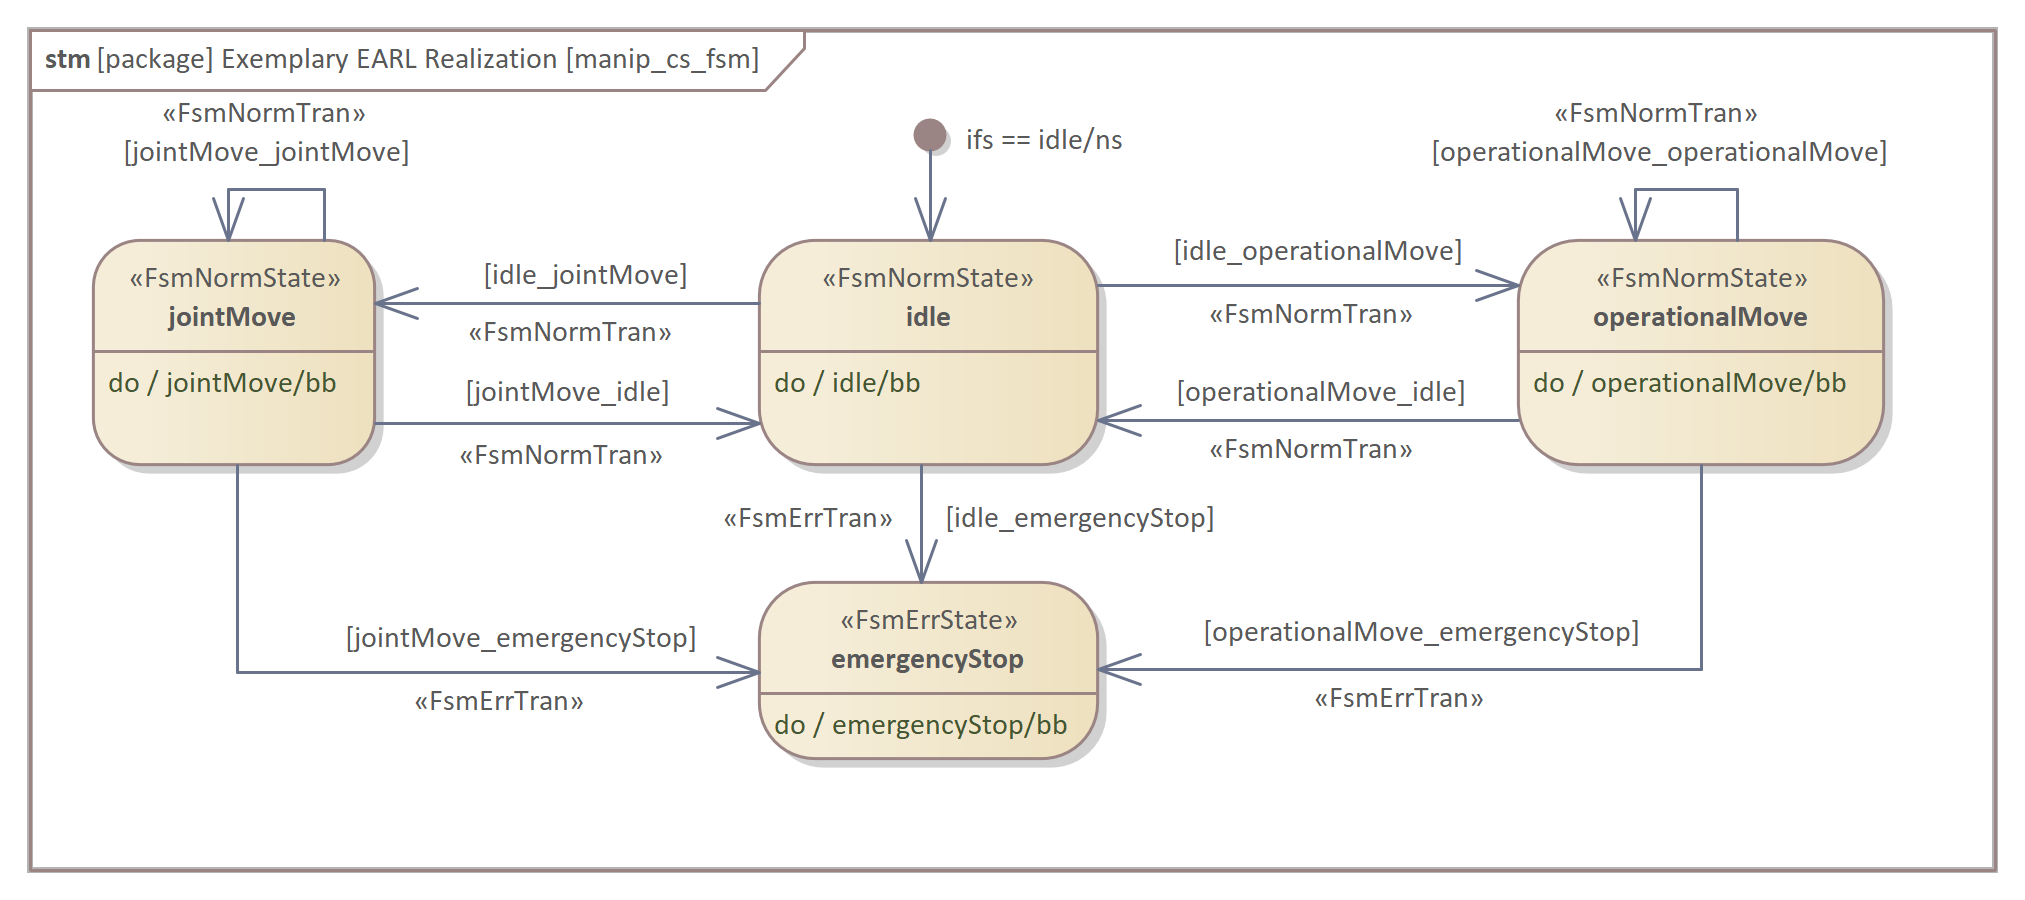
\includegraphics[width=\columnwidth]{img/basic_earl_instance/manip_cs_fsm.png}}
		\end{center}
		\caption{$\protect\ea{manip}.\protect\ecs{}.\protect\efsm{}$ definition. Conditions of transitions between \FsmStates{} are specified in \Table{}~\ref{tab:am-cs-fsm-t}}
		\label{fig:state_machines_a_m}
	\end{figure}
	
	\begin{figure}[H]
		\centering
		\begin{center}
			{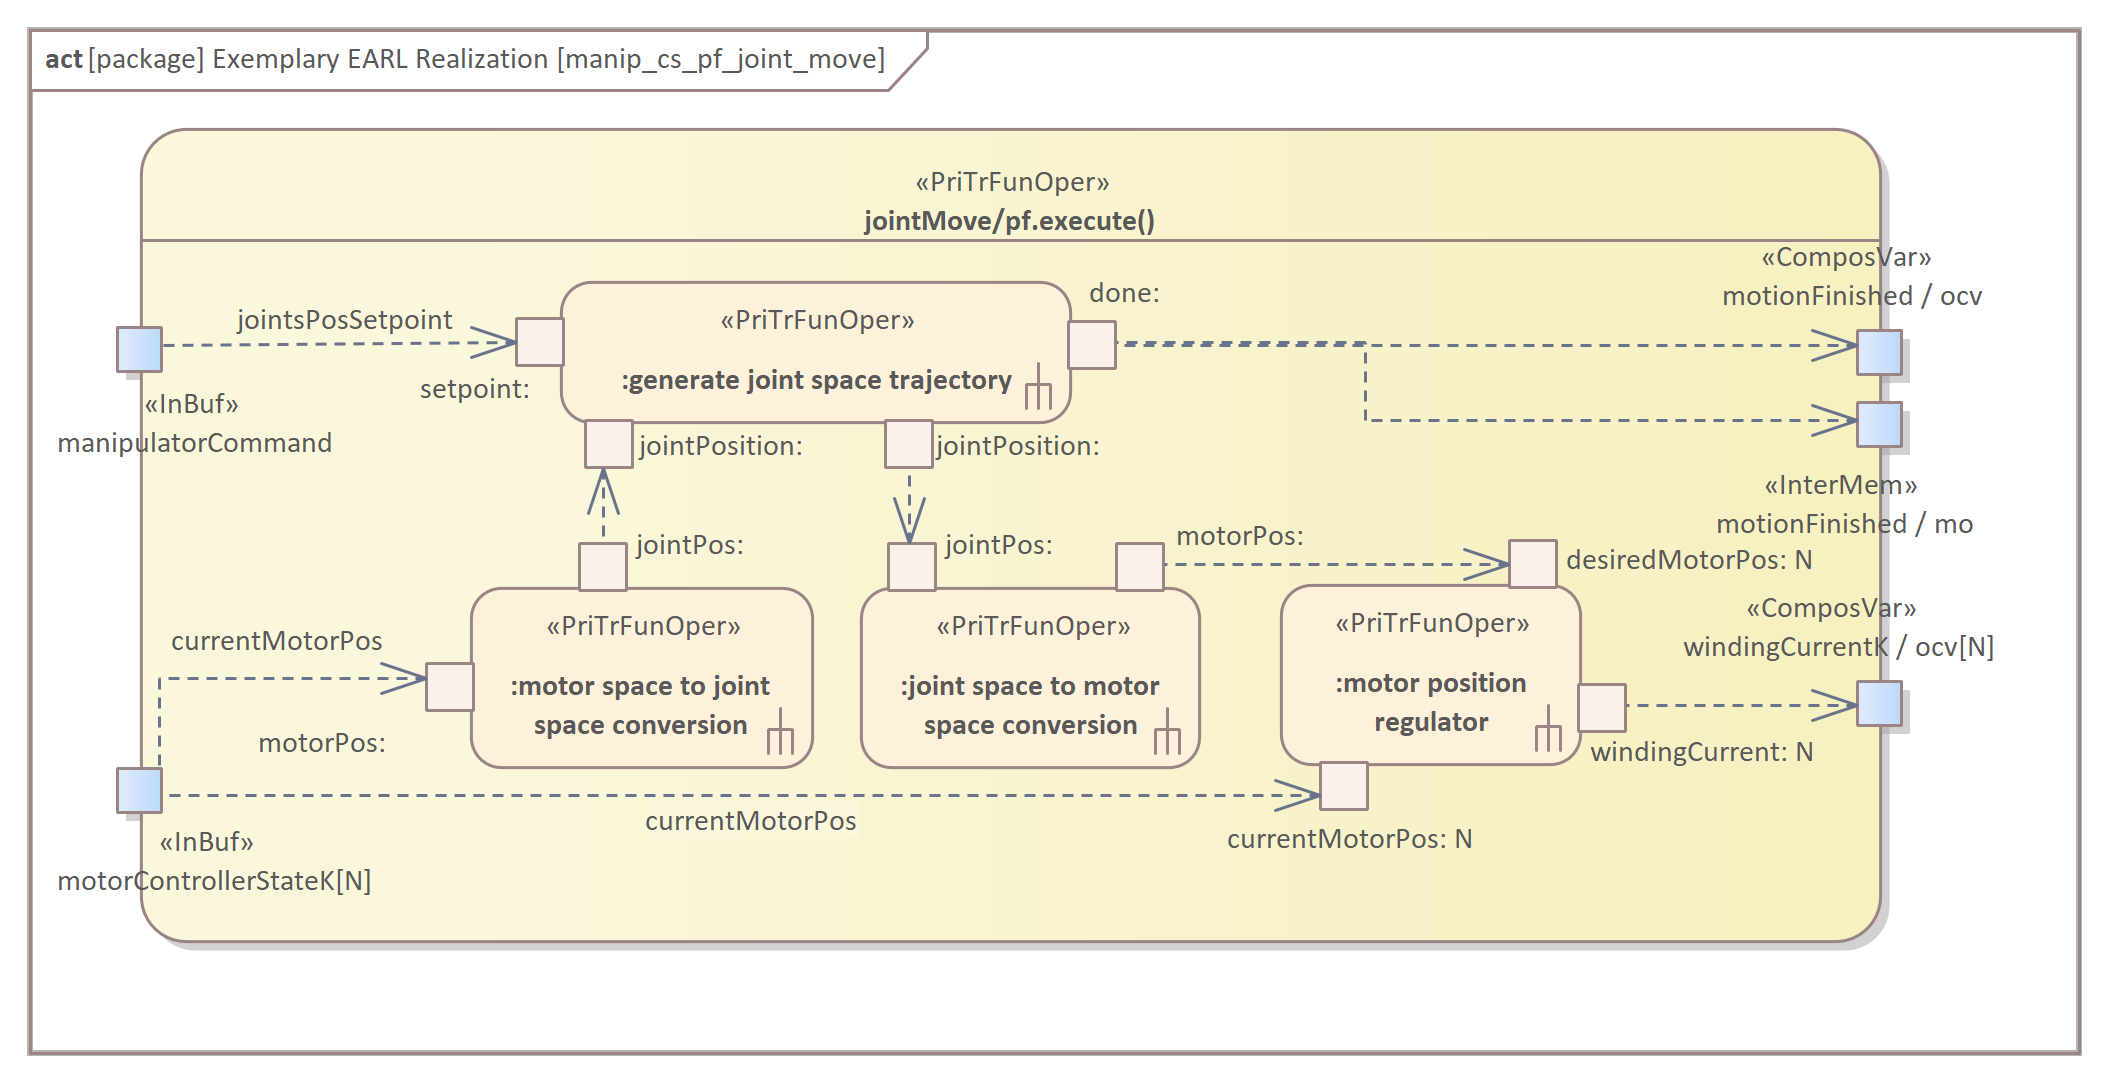
\includegraphics[width=\columnwidth]{img/basic_earl_instance/manip_cs_pf_joint_move.png}}
		\end{center}
		\caption{$\protect\ea{manip}.\protect\ecs{}.\protect\epf{jointMove}.execute()$ -- operation definition}
		\label{fig:confiop}
	\end{figure}
	
	\Figure{}~\ref{fig:confiop} shows the execute operation of a~$\epf{jointMove}$ \PrimitiveTransitionFunction{}. This \PrimitiveTransitionFunction{}
	realises, e.g., the PI type \textit{motor position regulator} for each joint Equation~\eqref{eq:pi1}, Equation~\eqref{eq:pi2}:
	\begin{equation}
	windingCurrent = K_p \, e(t) + K_i\int_{0}^{t}e(t')dt',
	\label{eq:pi1}
	\end{equation}
	\begin{equation}
	e = desiredMotorPos - currentMotorPos,
	\label{eq:pi2}
	\end{equation}
	where $K_p$ and $K_i$ are, respectively, proportional and integral gain factors, $e$ is the position error, $t$~is~time.
	
	\begin{figure}[H]
		\def\myheight{6cm}
		\centering
		\subfloat[$\protect\epf{outputManipState}.execute()$ \label{fig:manip_cs_compose_ms}]{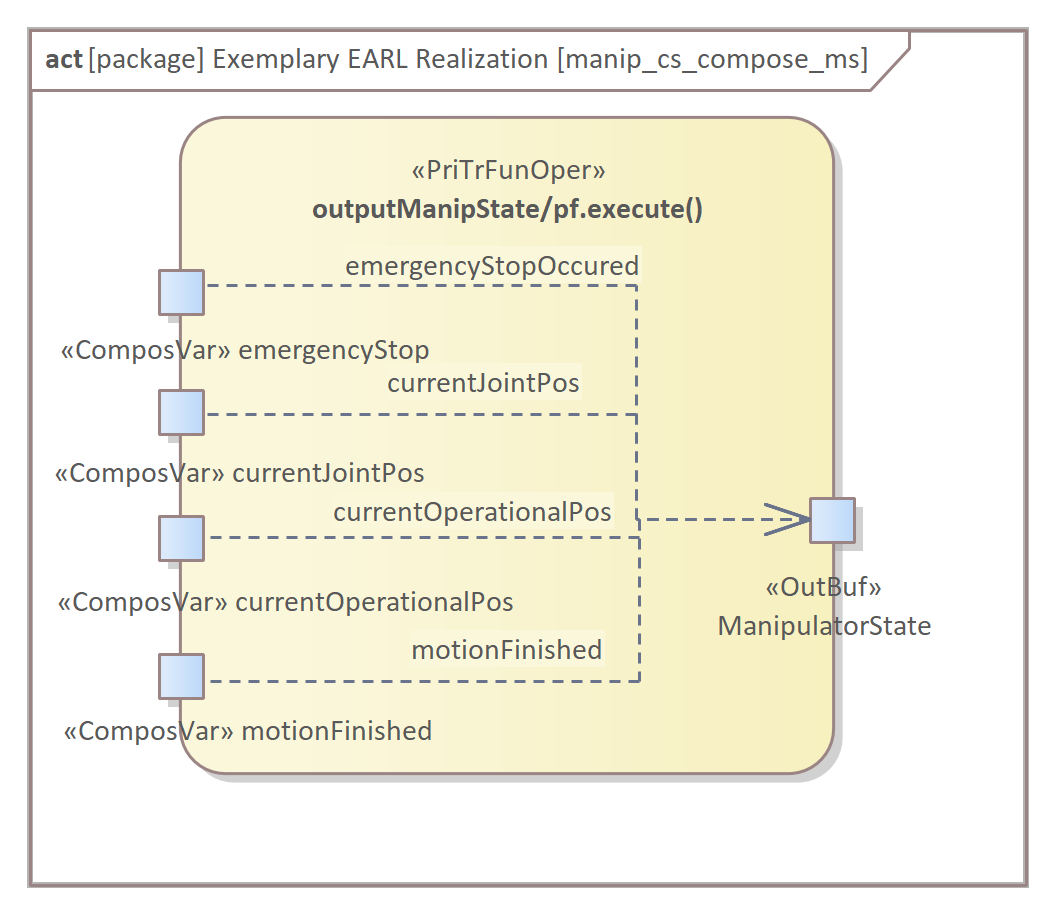
\includegraphics[height=\myheight]{img/basic_earl_instance/manip_cs_compose_ms.png}} \quad
		\subfloat[$\protect\epf{outputMotorCon}.execute()$ \label{fig:manip_cs_compose_dc}]{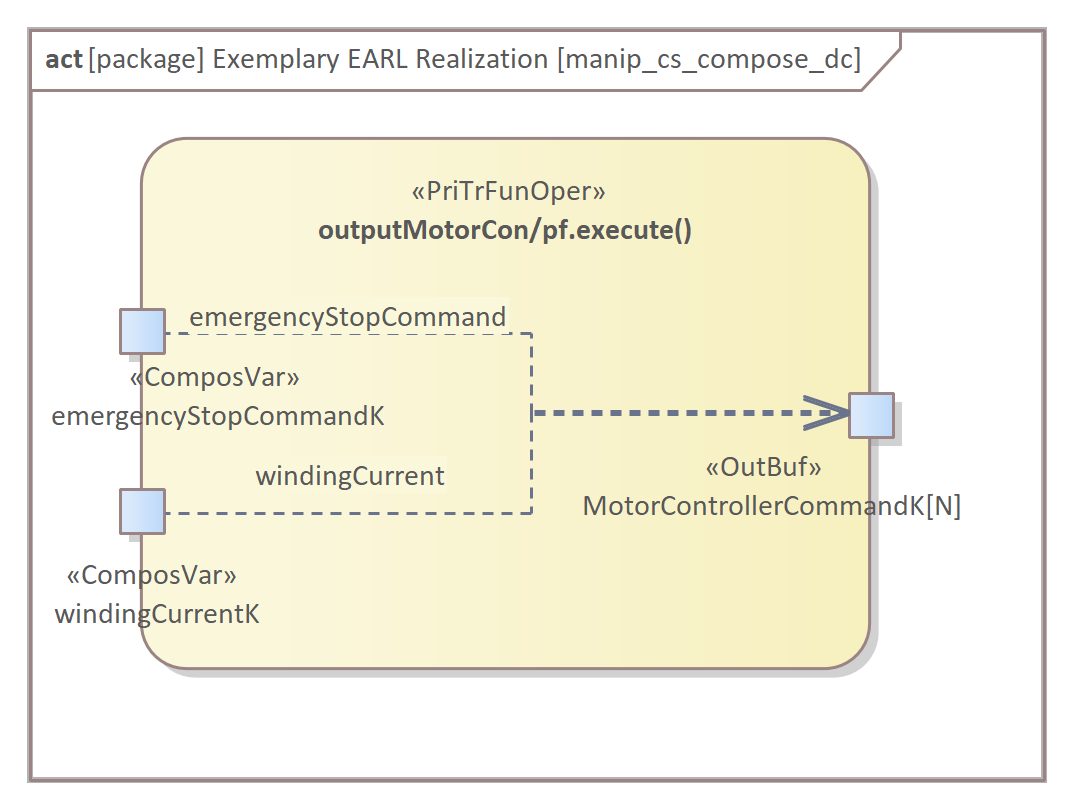
\includegraphics[height=\myheight]{img/basic_earl_instance/manip_cs_compose_dc.png}}
		\caption{$\protect\ea{manip}.\protect\ecs{}.\protect\epf{}.execute()$ -- operations definition}
		\label{fig:pfo-execute}
	\end{figure}
	Figures~\ref{fig:manip_cs_compose_ms} and~\ref{fig:manip_cs_compose_dc} show the execute operation of a~$\epf{outputManipState}$ and $\epf{outputMotorCon}$ respectively. Those \PrimitiveTransitionFunctions{} define the composition of \OutputBuffer{} messages from certain \TransitionFunctionCompositionVariables{} entities.

	\begin{figure}[H]
		\centering
		\begin{center}
			{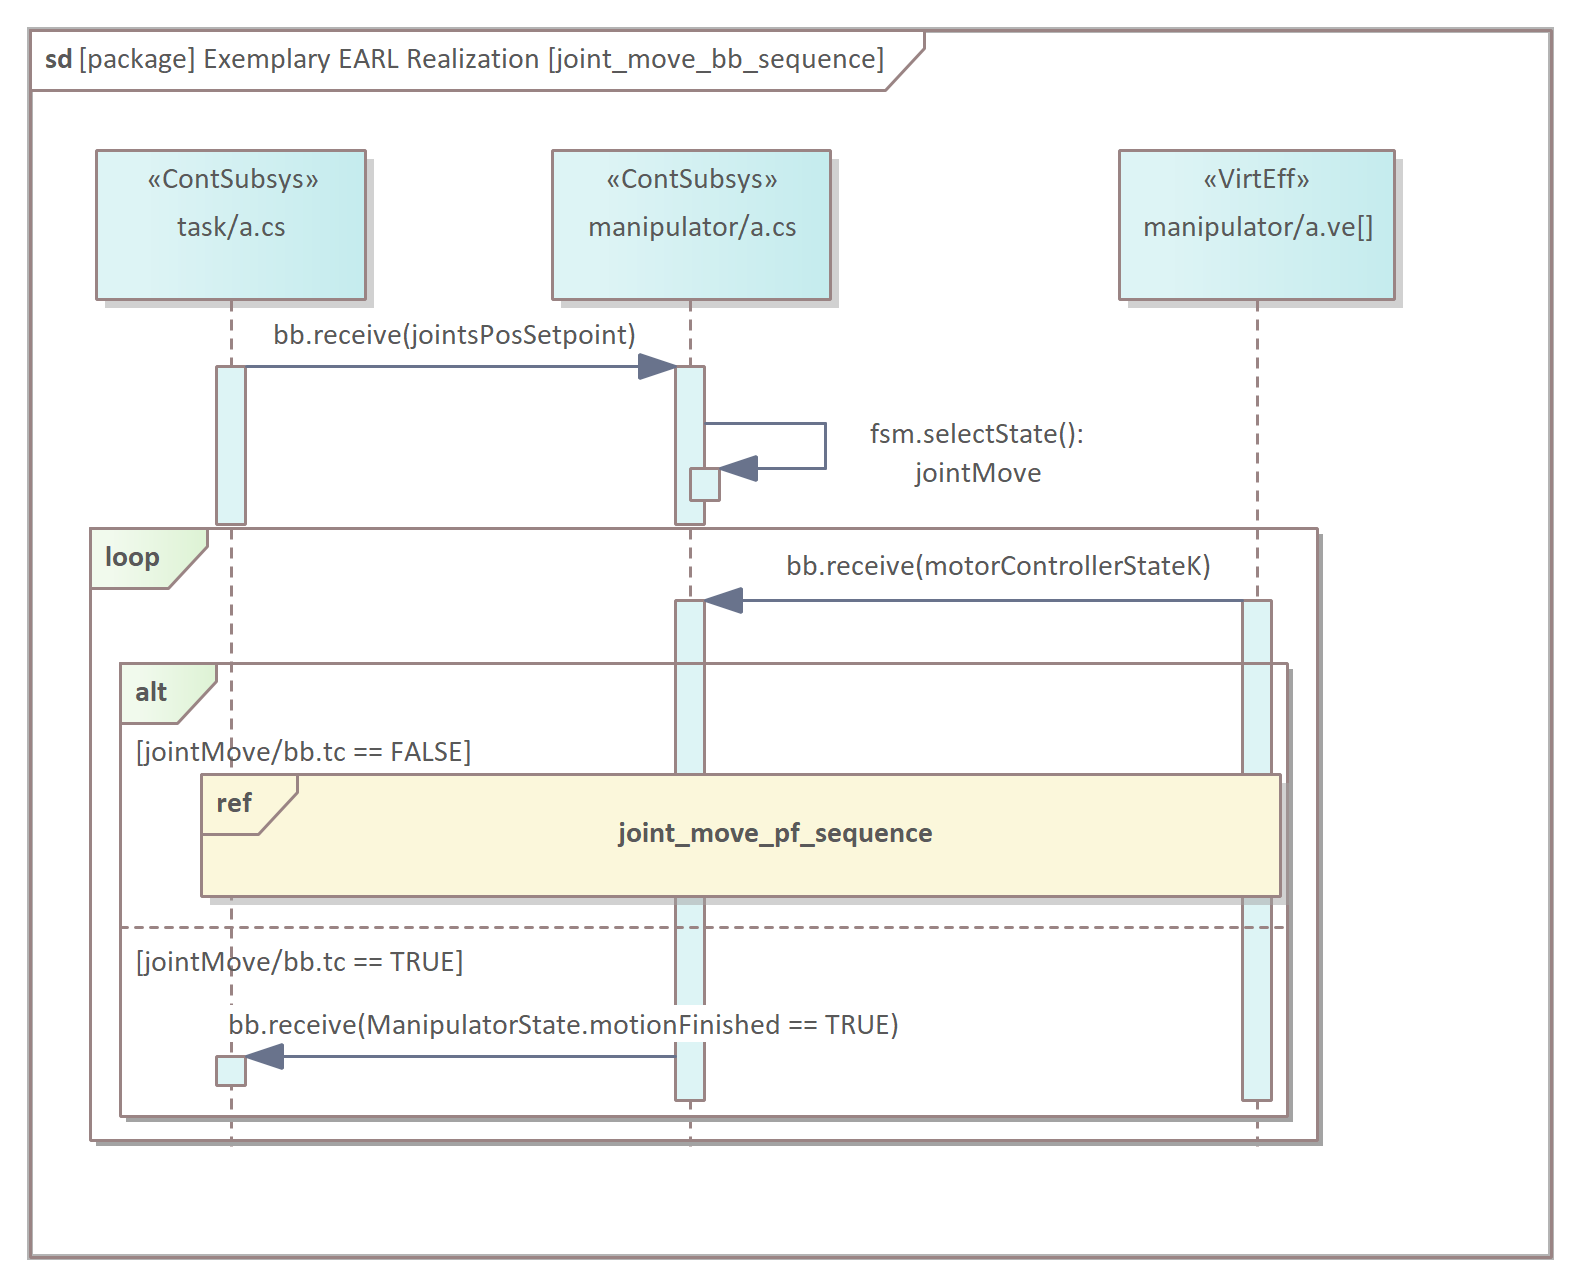
\includegraphics[width=0.7\columnwidth]{img/basic_earl_instance/joint_move_bb_sequence.png}}
		\end{center}
		\caption{$\protect\ebb{jointMove}$ -- main sequence of actions execution}
		\label{fig:joint_move_bb_sequence}
	\end{figure}

	\begin{figure}[H]
	\centering
	\begin{center}
		{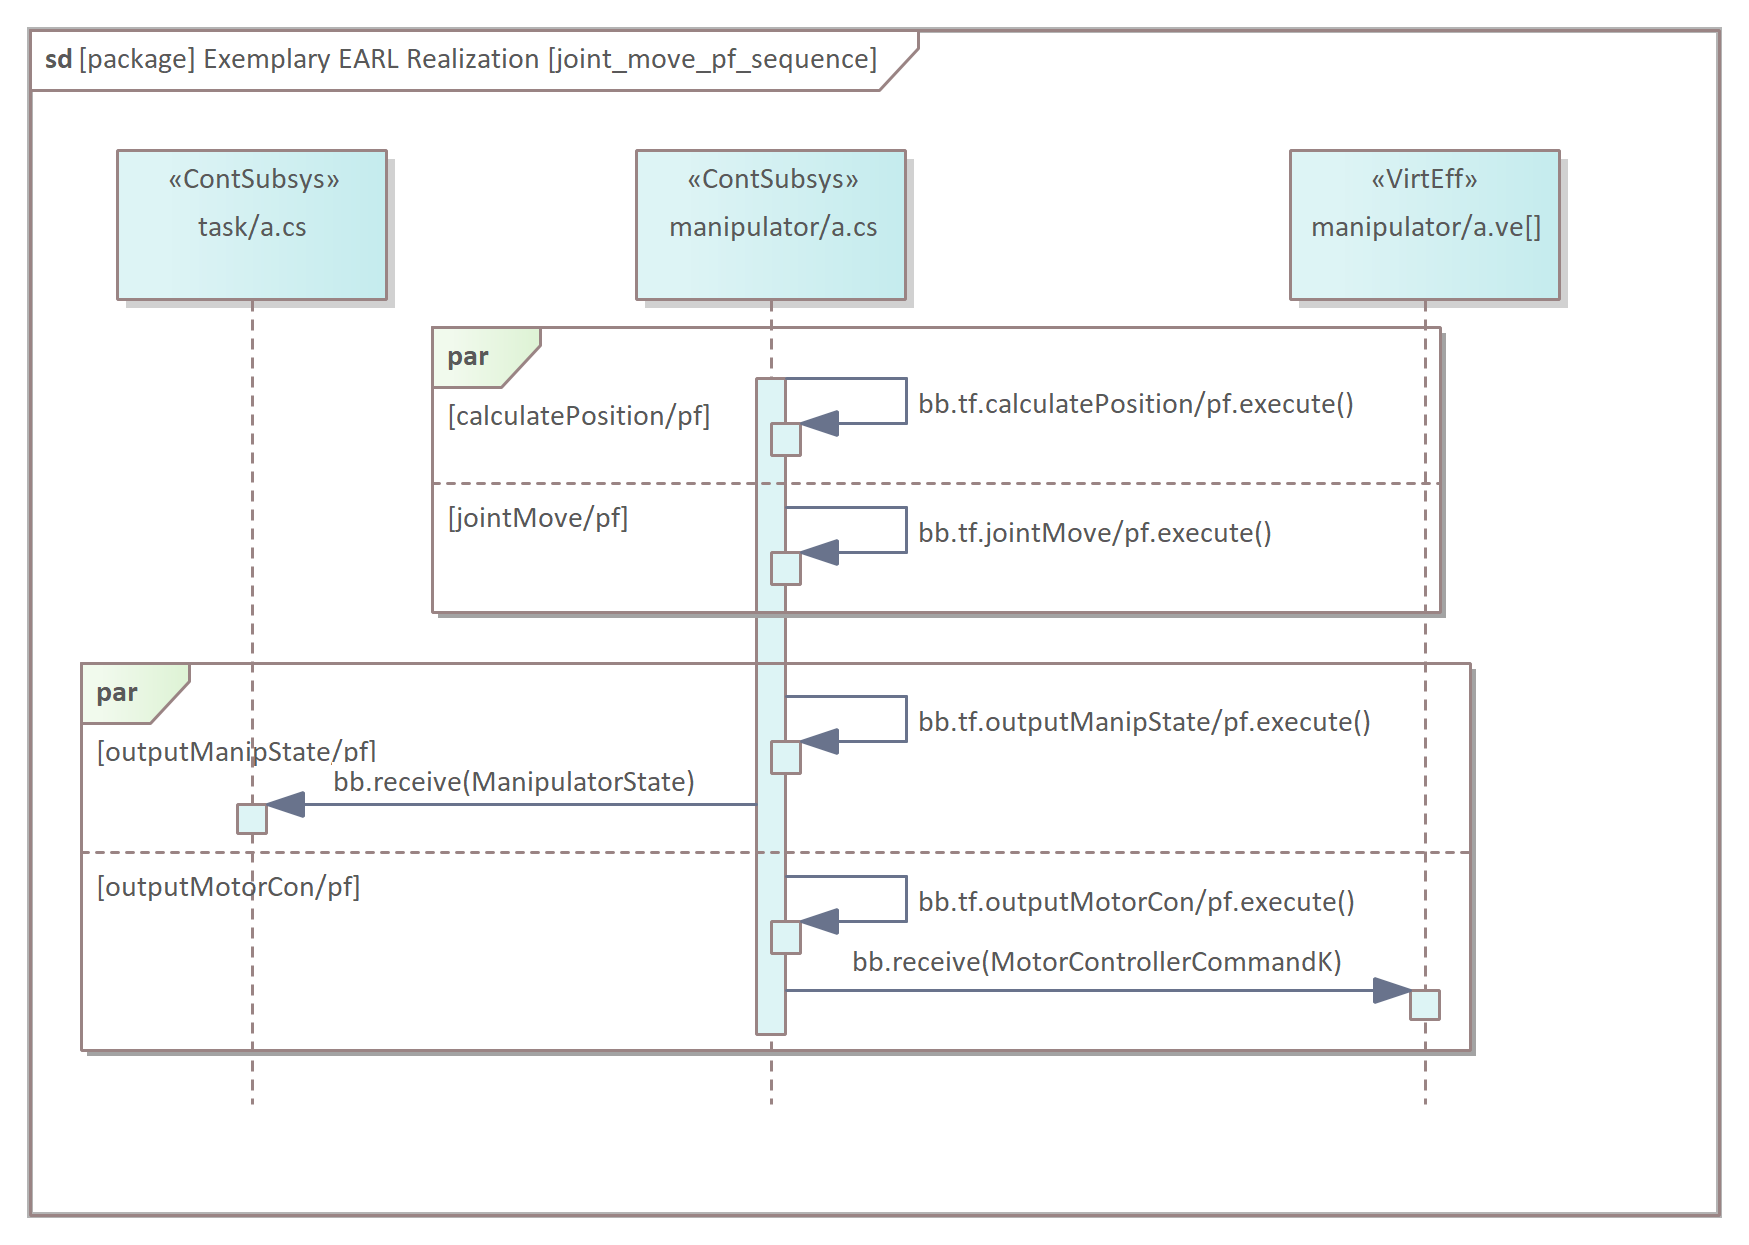
\includegraphics[width=0.7\columnwidth]{img/basic_earl_instance/joint_move_pf_sequence.png}}
	\end{center}
	\caption{$\protect\ebb{jointMove}$ -- main sequence of associated $\protect\epf{}$ execution}
	\label{fig:joint_move_pf_sequence}
	\end{figure}

	Figures~\ref{fig:joint_move_bb_sequence} and~\ref{fig:joint_move_pf_sequence} show how the operations $\epf{jointMove}$, $\epf{calculatePosition}$, $\epf{outputManipState}$ and $\epf{outputMotorCon}$ are executed. In particular it shows:
	\begin{itemize}
		\item the order of $\epf{}$ execution, and
		\item moments when communication with associated subsystems takes place.
	\end{itemize}
	
	\Table{}~\ref{tab:zachstany1} shows which \PrimitiveTransitionFunctions{} constitute the composition of transition function used by \BasicBehaviours{} of $\ea{manip}.\ecs{}.\ebb{}$.
	
	The \PrimitiveTransitionFunctions{} $\ea{manip}.\ecs{}.\epf{}$ composed into \PrimitiveTransitionFunction{} $\ea{manip}.\ecs{}.\ebb{}.\etf{}$ are subdivided into two disjoint sets: $\epfc{}$ and $\epfo{}$. The $\epfc{}$ set Equation \eqref{eq:pfc}
	contains \PrimitiveTransitionFunctions{} that take as arguments \InputBuffers{}: $\eib{manipulatorCommand}$ and\\ $\eib{motorControllerCommandK}[N]$
	\begin{equation}
	\begin{split}
	\epfc{}\!=\!\{\epf{calculatePosition}, \epf{jointMove}, \epf{operationalMove}, \\ \epf{passiveRegulation}, \epf{emergencyStop}\}.
	\end{split}
	\label{eq:pfc}
	\end{equation}
	The values produced
	by them are inserted into the \TransitionFunctionCompositionVariables{} $\eocvs{}$ Equation~\eqref{eq:ocvs}
	\begin{equation}
	\begin{split}
	\eocvs{}\!=\!\{\eocv{motionFinished}, \eocv{currentOperationalPos}, \eocv{currentJointsPos}, \\ \eocv{emergencyStopCommandK}, \eocv{windingCurrentK}\}.
	\end{split}
	\label{eq:ocvs}
	\end{equation}
	and the \InternalMemory{} $\embo{}$ Equation~\eqref{eq:mbo}
	\begin{equation}
		\begin{split}
			\embo{}\!=\!\{\emo{motionFinished}\}.
		\end{split}
		\label{eq:mbo}
	\end{equation}
	Functions from the $\epfo{}$ set Equation~\eqref{eq:pfo} take arguments from the \TransitionFunctionCompositionVariables{} $\eicvs{}$ associated with these  from set $\eocvs{}$ Equation~\eqref{eq:ocvs} and produce the \OutputBuffer{} values:
	$\eob{ManipulatorState}$ and $\eob{MotorControllerCommandK}[N]$, hence they produce output of the whole \Subsystem{}
	\begin{equation}
	\epfo{}\!=\!\{\epf{outputManipState}, \epf{outputMotorCon}\}.
	\label{eq:pfo}
	\end{equation}
	It was assumed that any two \PrimitiveTransitionFunctions{} used by a~particular \PrimitiveTransitionFunction{} $\ea{manip}.\ecs{}.\ebb{}.\etf{}$ do not produce data to the same \TransitionFunctionCompositionVariables{}, \InternalMemories{} and \OutputBuffers{},
	therefore the following conditions are formulated for the $\epfc{}$ set Equations~\eqref{eq:pfc-composition-condition1},~\eqref{eq:pfc-composition-condition2} and the $\epfo{}$ set Equation~\eqref{eq:pfo-composition-condition}, respectively,
	\begin{equation}
	(\forall \ebb{x})(\forall \ebb{x}.\epf{i}, \ebb{x}.\epf{j} \in \epfc{}, \; i~\neq j) (\ebb{x}.\epf{i}.\eocv{k} \nsim \ebb{x}.\epf{j}.\eocv{k}, \; \eocv{k} \in \eocvs{}),
	\label{eq:pfc-composition-condition1}
	\end{equation}
	\begin{equation}
	(\forall \ebb{x})(\forall \ebb{x}.\epf{i}, \ebb{x}.\epf{j} \in \epfc{}, \; i~\neq j) (\ebb{x}.\epf{i}.\emo{k} \nsim \ebb{x}.\epf{j}.\emo{k}, \; \emo{k} \in \embo{}),
	\label{eq:pfc-composition-condition2}
	\end{equation}
	\begin{equation}
	(\forall \ebb{x})(\forall \ebb{x}.\epf{i}, \ebb{x}.\epf{j} \in \epfo{}, \; i~\neq j) (\ebb{x}.\epf{i}.\eob{k} \nsim \ebb{x}.\epf{j}.\eob{k}),
	\label{eq:pfo-composition-condition}
	\end{equation}
	where $\nsim$ stands for ,,is not the same entity''.
	
	\begin{table}[H]
		\centering
		\small
		\caption{Aggregation of transition function $\protect\ea{manip}.\protect\ecs{}.\protect\ebb{}.\protect\etf{}$ with \mbox{\PrimitiveTransitionFunctions{}} $\protect\ea{manip}.\protect\ecs{}.\protect\bbb{}.\protect\etf{}.\protect\bpf{}$. The right part of the table presents
			what parts of \OutputBuffers{}, \TransitionFunctionCompositionVariables{} and \InternalMemories{} are produced by the specific \mbox{\PrimitiveTransitionFunctions{}}}
		\scalebox{.9}[.9]{	\begin{tabular}[]{p{3.1cm} p{3.5cm}| p{0.4cm} p{0.4cm} p{0.4cm} p{0.4cm} p{0.4cm} | p{0.4cm} | p{0.4cm} p{0.4cm}}
				\noalign{\hrule height 1.0pt} 
				\multicolumn{2}{c|}{}&\multicolumn{5}{c|}{$/\eocv{}$}&\multicolumn{1}{c|}{$/\emo{}$}&\multicolumn{2}{c}{$/\eob{}$} \\ 
				\makecell{$/\bbb{}$} & \makecell{$/\bpf{}$} & \rotatebox{90}{$ motionFinished$} & \rotatebox{90}{$ currentJointPos$} &\rotatebox{90}{$ currentOperationalPos$} & \rotatebox{90}{$ emergencyStop$} & \rotatebox{90}{$ windingCurrentK$}& \rotatebox{90}{$ motionFinished$} & \rotatebox{90}{$ ManipulatorState$} & \rotatebox{90}{$ MotorControllerCommandK$\hspace{.1cm}}\\ 
				\hline	
				
				
				&&&&&&&&&\\[-6pt]
				
				\makecell{\multirow{4}{*}{\makecell{$idle$}}}
				& \makecell{$outputManipState$} &$\m{}$&$\m{}$&$\m{}$&$\m{}$&$\m{}$&$\m{}$&$\p{}$&$\m{}$\\
				&&&&&&&&\\[-6pt]
				& \makecell{$outputMotorCon$} &$\m{}$&$\m{}$&$\m{}$&$\m{}$&$\m{}$&$\m{}$&$\m{}$&$\p{}$\\	
				&&&&&&&&\\[-6pt]
				& \makecell{$calculatePosition$} &$\m{}$&$\p{}$&$\p{}$&$\m{}$&$\m{}$&$\m{}$&$\m{}$&$\m{}$\\	
				&&&&&&&&\\[-6pt]
				& \makecell{$passiveRegulation$} &$\m{}$&$\m{}$&$\m{}$&$\m{}$&$\p{}$&$\m{}$&$\m{}$&$\m{}$\\ 
				\hline
				&&&&&&&&\\[-6pt]
				\makecell{\multirow{4}{*}{\makecell{$jointMove$}}}
				& \makecell{$outputManipState$} &$\m{}$&$\m{}$&$\m{}$&$\m{}$&$\m{}$&$\m{}$&$\p{}$&$\m{}$\\
				&&&&&&&&\\[-6pt]
				& \makecell{$outputMotorCon$} &$\m{}$&$\m{}$&$\m{}$&$\m{}$&$\m{}$&$\m{}$&$\m{}$&$\p{}$\\
				&&&&&&&&\\[-6pt]
				& \makecell{$calculatePosition$} &$\m{}$&$\p{}$&$\p{}$&$\m{}$&$\m{}$&$\m{}$&$\m{}$&$\m{}$\\
				&&&&&&&&\\[-6pt]
				& \makecell{$jointMove$} &$\p{}$&$\m{}$&$\m{}$&$\m{}$&$\p{}$&$\p{}$&$\m{}$&$\m{}$\\ 	
				\hline
				&&&&&&&&\\[-6pt]
				\makecell{\multirow{4}{*}{\makecell{$operationalMove$}}}
				& \makecell{$outputManipState$} &$\m{}$&$\m{}$&$\m{}$&$\m{}$&$\m{}$&$\m{}$&$\p{}$&$\m{}$\\
				&&&&&&&&\\[-6pt]
				& \makecell{$outputMotorCon$} &$\m{}$&$\m{}$&$\m{}$&$\m{}$&$\m{}$&$\m{}$&$\m{}$&$\p{}$\\	
				&&&&&&&&\\[-6pt]
				& \makecell{$calculatePosition$} &$\m{}$&$\p{}$&$\p{}$&$\m{}$&$\m{}$&$\m{}$&$\m{}$&$\m{}$\\	
				&&&&&&&&\\[-6pt]
				& \makecell{$operationalMove$} &$\p{}$&$\m{}$&$\m{}$&$\m{}$&$\p{}$&$\m{}$&$\m{}$&$\m{}$\\	
				\hline
				&&&&&&&&\\[-6pt]
				\makecell{\multirow{4}{*}{\makecell{$emergencyStop$}}}
				& \makecell{$outputManipState$} &$\m{}$&$\m{}$&$\m{}$&$\m{}$&$\m{}$&$\m{}$&$\p{}$&$\m{}$\\
				&&&&&&&&\\[-6pt]
				& \makecell{$outputMotorCon$} &$\m{}$&$\m{}$&$\m{}$&$\m{}$&$\m{}$&$\m{}$&$\m{}$&$\p{}$\\
				&&&&&&&&\\[-6pt]
				& \makecell{$calculatePosition$} &$\m{}$&$\p{}$&$\p{}$&$\m{}$&$\m{}$&$\m{}$&$\m{}$&$\m{}$\\
				&&&&&&&&\\[-6pt]
				& \makecell{$emergencyStop$} &$\m{}$&$\m{}$&$\m{}$&$\p{}$&$\m{}$&$\m{}$&$\m{}$&$\m{}$\\ 
				\noalign{\hrule height 1.0pt} 
		\end{tabular}}
		\label{tab:zachstany1}
	\end{table}	
	
	Transition functions $\ea{manip}.\ecs{}.\ebb{}.\etf{}$ act in the following way. First, they compute the \PrimitiveTransitionFunctions{} from the $\epfc{}$ set, and then they compute the \PrimitiveTransitionFunctions{} from the $\epfo{}$ set.
	The fulfilment of Equations \eqref{eq:pfc-composition-condition1},~\eqref{eq:pfc-composition-condition2} and \eqref{eq:pfo-composition-condition} makes it possible to run \PrimitiveTransitionFunctions{}
	being members of $\epfc{}$ in parallel in the first stage of the \PrimitiveTransitionFunction{} $\ea{manip}.\ecs{}.\ebb{}.\etf{}$ execution, and then run the \PrimitiveTransitionFunctions{} being members of $\epfo{}$ set in parallel in the
	second stage of \PrimitiveTransitionFunction{} $\ea{manip}.\ecs{}.\ebb{}.\etf{}$ execution. To illustrate the above considerations, \Figure{}~\ref{fig:bb_jointMove} shows the definition of
	$\ebb{jointMove}.\etf{}.execute()$ operation -- practical realisation of transition function execution for $jointMove$ \BasicBehaviour{}.
	
	
	\begin{figure}[H]
		\centering
		\begin{center}
			{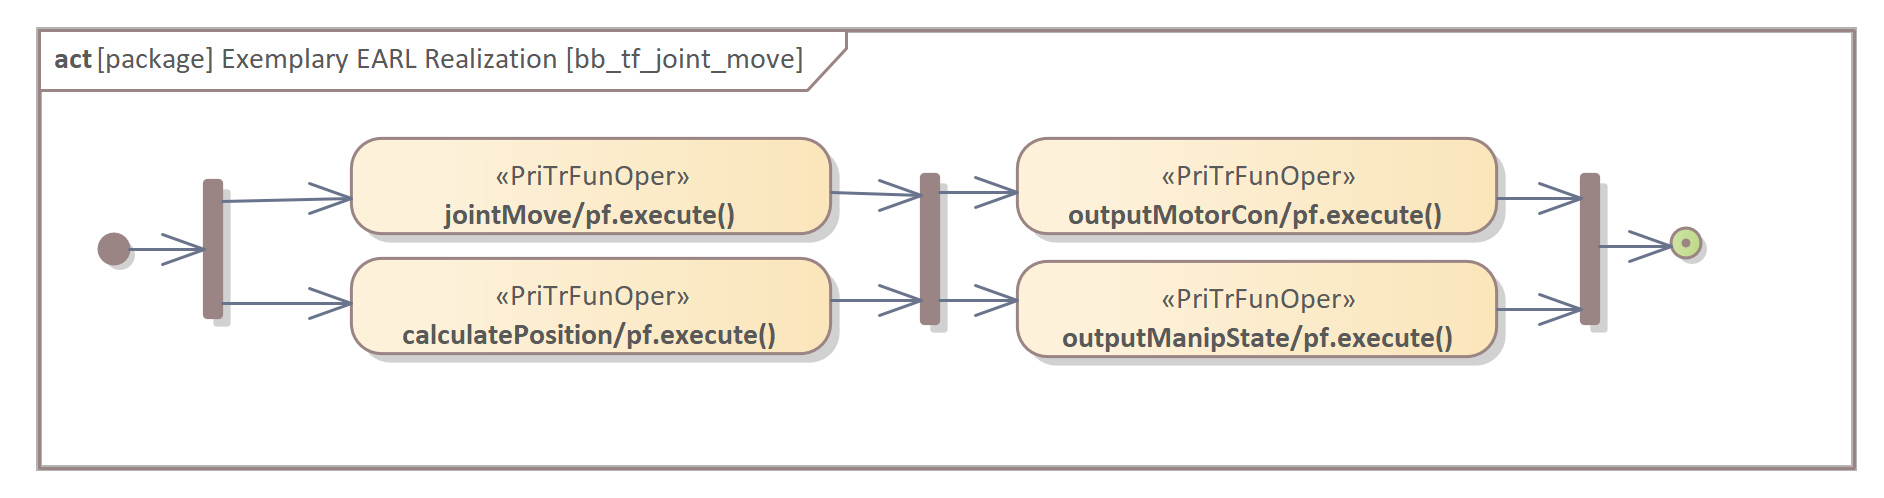
\includegraphics[width=0.9\columnwidth]{img/basic_earl_instance/bb_tf_joint_move.png}}
		\end{center}
		\caption{$\protect\ebb{jointMove}.\protect\etf{}.execute()$ operation definition}
		\label{fig:bb_jointMove}
	\end{figure}

\section{Exemplary \EARL{} customisations}
\label{sec:customisations}

The convenient way to customize \EARL{} model is to specify a~new model and include it in the dedicated SysML package. The Blocks of the new model can derive from Basic Model blocks.

\subsection{Agent specialisation}
\label{ssec:search-and-rescue}

The \Agent{} block can be specialised to, e.g., group \Agents{} with certain properties and to define communication structure of particular \System{}. The composition of exemplary Search and Rescue System is depicted in \Figure{}~\ref{fig:sar_bdd}.


\begin{figure}[H]
	\centering
	\begin{center}
		{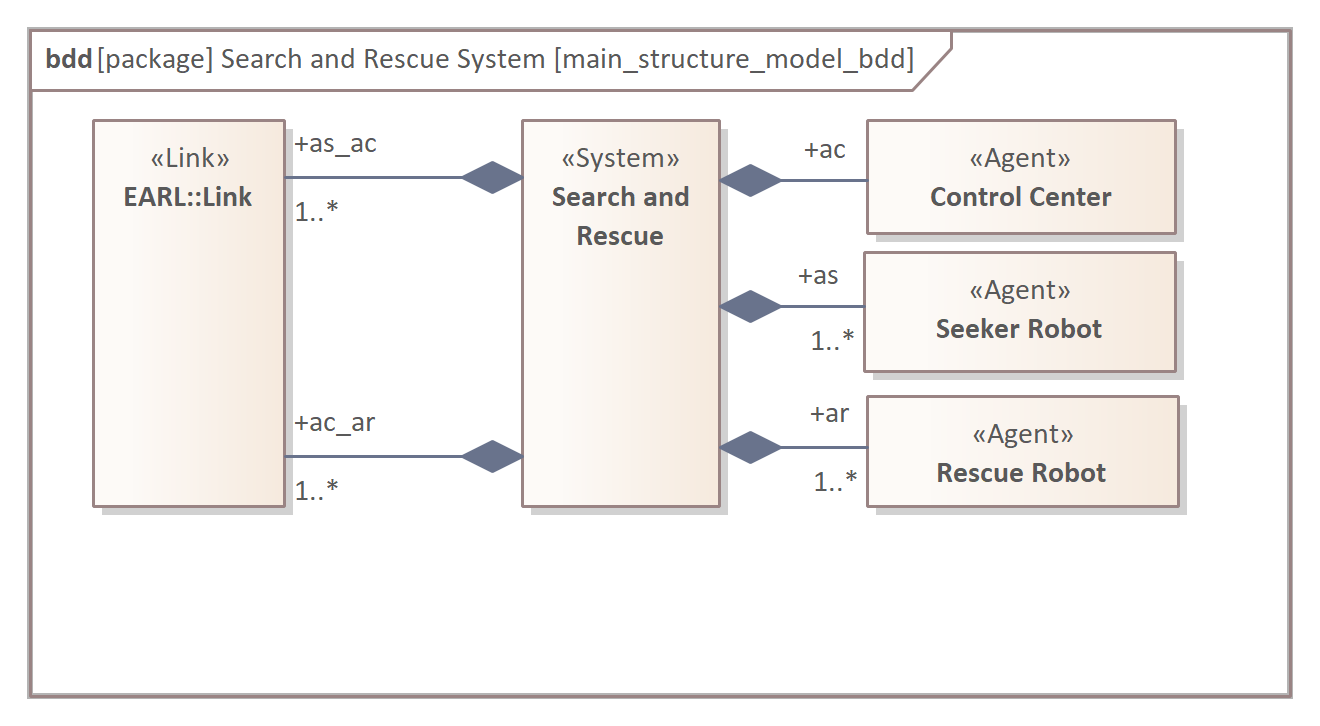
\includegraphics[width=0.7\columnwidth]{img/search_and_rescue_system_model/main_structure_model_bdd.png}}
	\end{center}
	\caption{The composition of Search and Rescue \System{}}
	\label{fig:sar_bdd}
\end{figure}

The communication structure and constraints are presented in \Figure{}~\ref{fig:sar_com_con}. Control Center Agent plays a~role of communication broker between Seeker Robot Agents and Rescue Robot Agents. The communication in this example is unidirectional.

\begin{figure}[H]
	\centering
	\begin{center}
		{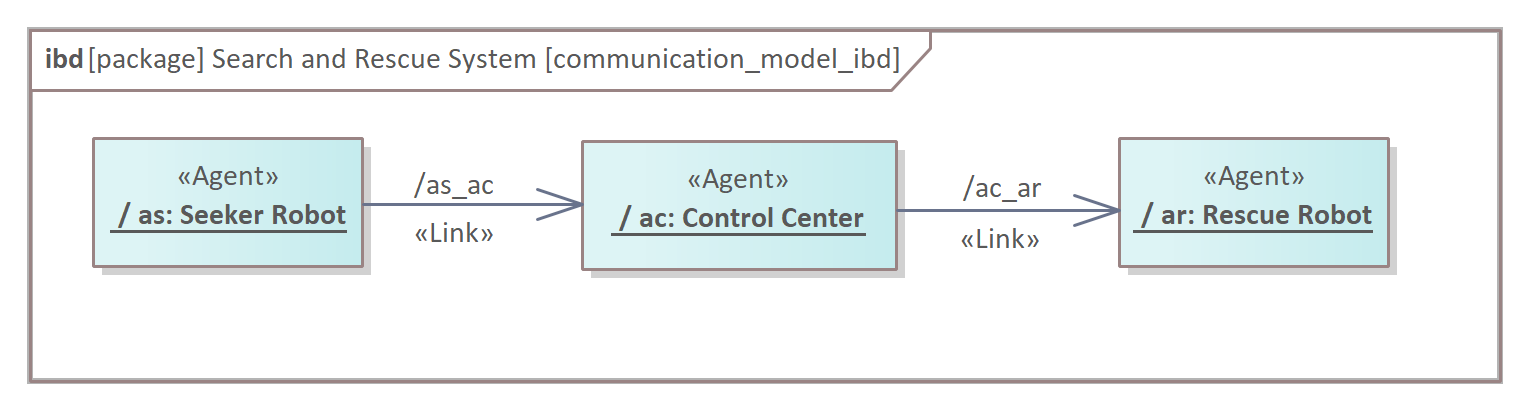
\includegraphics[width=0.8\columnwidth]{img/search_and_rescue_system_model/communication_model_ibd.png}}
	\end{center}
	\caption{The communication structure and constraints of Search and Rescue \System{}}
	\label{fig:sar_com_con}
\end{figure}



It should be noted that \System{} parts:~$\ea{}$,~$\eaa{}$ should not be used in the inherited \Systems{} without redefinition that keeps model consistency. In Search and Rescue System these parts are not redefined, so they are not used. Hence, the general structure of an exemplary instance of Search and Rescue \System{} may take form as in \Figure{}~\ref{fig:sar_instance_ibd}. It consists of: 3~seeker robots, 2~rescue robots, control centre and communication \Links{} between previously mentioned parts. It should be noted that for the sake of brief, general system structure description the ports have not to be directly specified in ibd, as well as \Links{} names. 


\begin{figure}[H]
	\centering
	\begin{center}
		{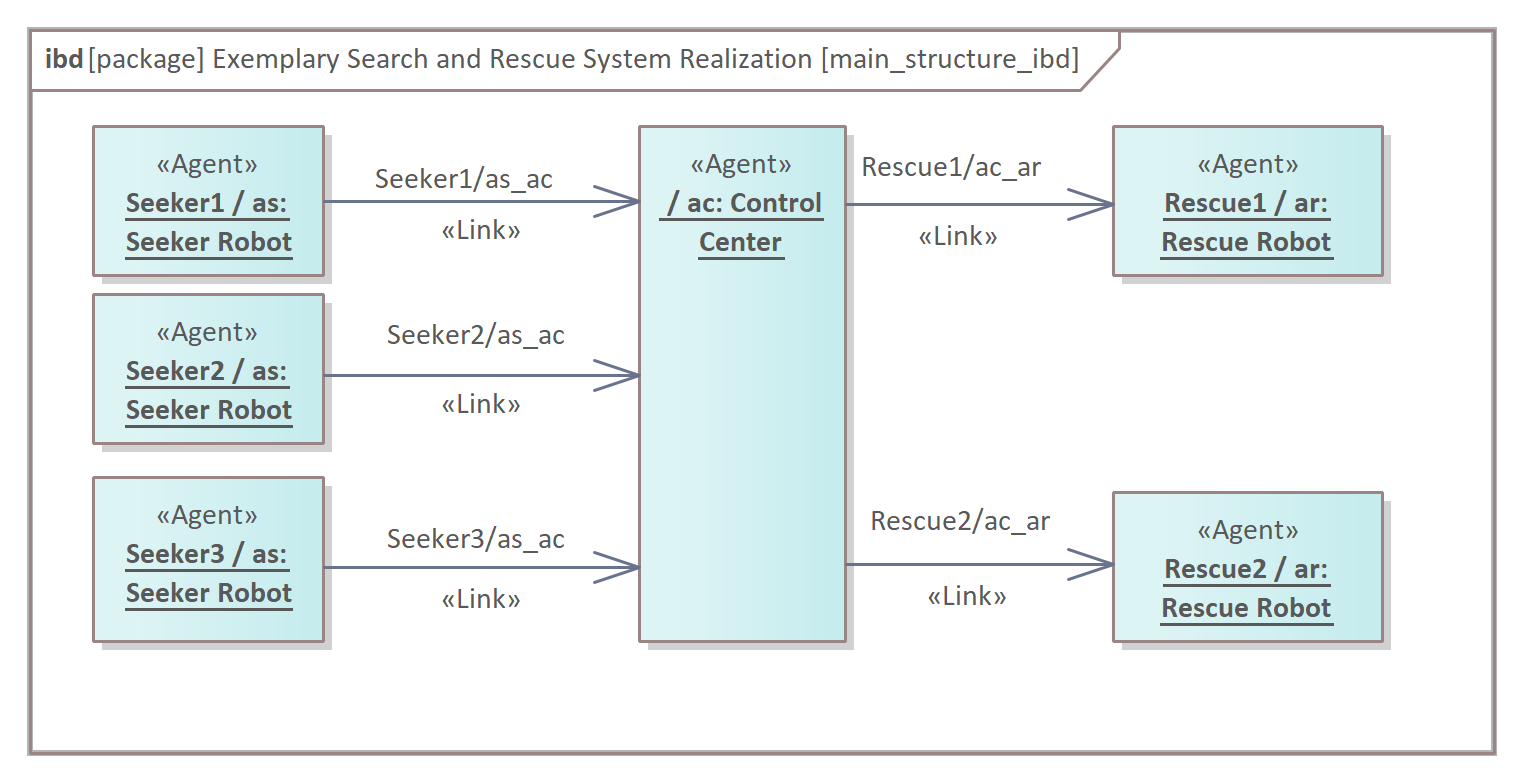
\includegraphics[width=0.8\columnwidth]{img/search_and_rescue_system_instance/main_structure_ibd.png}}
	\end{center}
	\caption{The structure of an exemplary instance of Search and Rescue \System{}}
	\label{fig:sar_instance_ibd}
\end{figure}



\section{Major changes in current version}
\label{sec:major-changes}

\begin{enumerate}
	\item Stereotypes introduced (authors: Tomasz Winiarski).
\end{enumerate}

\AtNextBibliography{\small}
\printbibliography

\end{document}

